\chapter{การประยุกต์ใช้โครงข่ายประสาทเทียม}
\label{chapter: Applications of ANN}

%\begin{multicols}{2}

\begin{verse}
``In theory there is no difference between theory and practice.
\\In practice there is.'' \\
---Yogi Berra
\end{verse}

\begin{verse}
``ในทางทฤษฎีแล้วไม่มีความแตกต่างระหว่างทฤษฎีกับการปฏิบัติ
\\แต่ในทางปฏิบัติแล้วต่าง''\\
%มีความแตกต่างอยู่''\\
---โยกี เบอร์ร่า
\end{verse}

%\end{multicols}

%“Practice isn't the thing you do when you're good. It's the thing you do that makes you good.” 
%? Malcolm Gladwell, Outliers: The Story of Success

%\begin{verse}
%``Mere philosophy will not satisfy us. 
%We cannot reach the goal by mere words alone. 
%Without practice, nothing can be achieved.''
%Swami Satchidananda, The Yoga Sutras
%\end{verse}

บท~\ref{chapter: ANN} อภิปรายการทำงานของโครงข่ายประสาทเทียม 
ว่าสามารถทำงานได้อย่างไรในมุมมองเชิงทฤษฎี.
อย่างไรก็ตาม การนำโครงข่ายประสาทเทียมไปใช้งานในทางปฏิบัติ ยังมีรายละเอียดอีกมาก ที่มีผลให้โครงข่ายประสาทเทียมสามารถทำงานได้อย่างมีประสิทธิภาพเพิ่มขึ้น
และบ่อยครั้งที่สำหรับการเรียนรู้ของเครื่องแล้วไม่ใช่เรื่องแปลกเลย 
ที่จะพบกรณีที่ความแตกต่าง ระหว่างความสามารถในการทำงานได้อย่างมีประสิทธิภาพกับไม่มีประสิทธิภาพ 
เทียบเท่าได้กับการทำงานได้หรือไม่ได้เลยทีเดียว.

ปัจจัยสำคัญเรื่องแรก คือ\textit{การกำหนดค่าเริ่มต้นของค่าน้ำหนัก} (weight initialization). \index{การกำหนดค่าเริ่มต้นของค่าน้ำหนัก} \index{weight initialization}
สังเกตุว่าโครงข่ายประสาทเทียมมีโครงสร้างที่มีความสมมาตรและมีรูปแบบซ้ำซ้อนกันเองอยู่ (แต่ละหน่วยประสาทเทียมมีสูตรการคำนวณเหมือนกัน) 
ดังนั้นถ้าหากกำหนดค่าเริ่มต้นของค่าน้ำหนัก เป็น $0$ ทั้งหมด ค่าน้ำหนักต่างๆแม้จะเป็นค่าของหน่วยประสาทคนละหน่วย 
แต่ก็จะถูกปรับปรุงไปเป็นค่าเหมือนๆกัน.
สุดท้ายแล้ว ไม่ว่าจะฝึกอย่างไร หรือโมเดลมีความลึกเท่าไร หรือมีจำนวนหน่วยซ่อนมากเท่าไร ผลที่ได้ก็คือโครงข่ายประสาทเทียมที่ค่าน้ำหนักเหมือนๆกันหลายๆค่า 
ซึ่งผลก็คือโครงข่ายประสาทเทียมจะไม่สามารถทำงานได้เต็มศักยภาพของมัน.
กล่าวง่ายๆ ในทางปฏิบัติแล้วการกำหนดค่าน้ำหนักเริ่มต้นเป็นศูนย์ทุกค่า 
จะทำให้การฝึกโครงข่ายประสาทเทียมล้มเหลว.
วิธีการกำหนดค่าเริ่มต้นของค่าน้ำหนักที่ง่ายที่สุด และสามารถทำงานได้อย่างมีประสิทธิภาพพอสมควร 
คือการสุ่มค่าเริ่มต้น ดังที่เราจะได้เห็นในตัวอย่าง (หัวข้อ~\ref{sec: simple example}).
%หัวข้อ~\ref{sec: Nguyen-Widrow Weight Initialization} พูดถึง 
ผู้อ่านที่สนใจศาสตร์และศิลป์ของการกำหนดค่าน้ำหนักเริ่มต้น สามารถศึกษา\textit{วิธีเหงี่ยน-วิดโดรว์} (Nguyen-Widrow Weight Initialization)  ซึ่งเป็นวิธีการกำหนดค่าเริ่มต้นของค่าน้ำหนักที่มีประสิทธิภาพมากขึ้นได้จากบทความของเหงี่ยนและวิดโดรว์\cite{NguyenWidrow1990a}.

นอกจากนั้นยังอีกประเด็นอื่นๆอีก ที่มีผลต่อประสิทธิภาพของการใช้งานโครงข่ายประสาทเทียม เช่น การทำการประมวลผลก่อนและหลัง (pre- and post-processing).
หัวข้อ~\ref{section: normalization} กล่าวถึงการทำนอร์มอไลเซชั่น ซึ่งเป็นการทำการประมวลผลก่อนอย่างหนึ่งที่นิยมมาก.

\section*{การทำนอร์มอไลเซชั่น}
\label{section: normalization}
\index{normalization}
\index{การทำนอร์มอไลเซชั่น}

\textit{การทำนอร์มอไลเซชั่น} (normalization) มีเหตุผลหลักอย่างหนึ่ง 
คือเพื่อปรับสเกลของค่าอินพุตมิติต่างๆกัน ให้มาอยู่ในช่วงค่าที่ใกล้เคียงกัน.
ตัวอย่างเช่น หากข้อมูลที่สนใจมี $2$ มิติ 
แต่มิติที่หนึ่งมีค่าอยู่ในช่วง $0.001$ ถึง $0.002$ 
ในขณะที่มิติที่สองกลับมีค่าอยู่ในช่วง $2000$ ถึง $4000$ 
เมื่อนำค่าของอินพุตเข้าไปฝึกโครงข่ายประสาทเทียมโดยตรง 
การฝึกอาจต้องใช้เวลานานมากที่น้ำหนักจะสามารถปรับตัวเองมา
เพื่อรักษาสมดุลของสเกลที่ต่างกันมากๆขนาดนี้ของอินพุตได้.
ไม่อย่างนั้น อินพุตมิติที่สองที่มีขนาดใหญ่กว่ามากอาจจะมีอิทธิพลกับเอาต์พุตมากจนอินพุตมิติที่หนึ่งไม่มีความหมาย
และส่งผลให้โมเดลไม่สามารถทำงานได้อย่างมีประสิทธิภาพ (เพราะเสมือนสร้างโมเดลจากอินพุตมิติที่สองเท่านั้น)

การทำนอร์มอไลเซชั่นสามารถทำได้หลายวิธี 
วิธีที่นิยมแบบที่หนึ่ง คือการปรับค่าให้ค่าอยู่ในช่วงที่กำหนด เช่น $[-1,1]$ หรือ $[0,1]$.
หากช่วงที่ต้องการคือ $[y_{\min}, y_{\max}]$ ค่าที่ทำนอร์มอไลเซชั่น $y$ สามารถคำนวณจาก
\[
   y = (y_{\max} - y_{\min}) \cdot \frac{x - x_{\min}}{x_{\max} - x_{\min}} + y_{\min}
\]
เมื่อ $x$ คือค่าเดิม 
และ
$x_{\min}$ กับ $x_{\min}$ คือค่าน้อยที่สุดกับค่ามากที่สุดของ $x$.
ตัวอย่างโค้ดสำหรับการทำนอร์มอไลเซชั่นแบบนี้แสดงในรายการ~\ref{lst: ann scg normalize}. %code is in the next chapter.

วิธีการทำนอร์มอไลเซชั่นที่นิยมแบบที่สอง คือการปรับค่าเพื่อให้ค่าเฉลี่ยและค่าเบี่ยงเบนมาตราฐาน เป็น $0$ กับ $1$ ตามลำดับ.
ดังนั้น ค่าที่ทำนอร์มอไลเซชั่น $y$ สามารถคำนวณได้จาก
\[
   y = \frac{x - \bar{x}}{\sigma_x}
\]
เมื่อ $\bar{x}$ และ $\sigma_x$ คือค่าเฉลี่ยและค่าเบี่ยงเบนมาตราฐาน ของ $x$ (ค่าเดิมก่อนทำนอร์มอไลเซชั่น).
ตัวอย่างโค้ดสำหรับการทำนอร์มอไลเซชั่นเพื่อปรับค่าเฉลี่ยนและค่าเบี่ยงเบนมาตราฐานแสดงในรายการ~\ref{lst: ann normalize}.

หมายเหตุ การทำนอร์มอไลเซชั่นทำเพื่อปรับสเกลของมิติต่างๆให้สมดุลกัน 
ดังนั้นการทำนอร์มอไลเซชั่นจะทำแต่ละมิติ 
เช่น หากมีสองมิติ $\mathbf{x} = [x_1, x_2]^T$ และหากต้องการทำนอร์มอไลเซชั่นให้อยู่ในช่วง $[0,1]$ ทั้งคู่ ก็ทำได้โดยแยกทำนอร์มอไลเซชั่นสำหรับแต่ละมิติซึ่งจะได้
\[
   \mathbf{y} = \begin{bmatrix}
   y_1 \\
   y_2
   \end{bmatrix}
   = \begin{bmatrix}
   (x_1 - {x_1}_{\min})/({x_1}_{\max} - {x_1}_{\min}) \\
   (x_2 - {x_2}_{\min})/({x_2}_{\max} - {x_2}_{\min}) \\
   \end{bmatrix}
\]
เมื่อ 
$y_1$ และ $y_2$ คือค่าที่ทำนอร์มอไลเซชั่นแล้วของมิติที่หนึ่งและสองตามลำดับ
${x_1}_{\min}$ กับ ${x_1}_{\min}$ คือค่าน้อยที่สุดกับค่ามากที่สุดของอินพุตมิติที่หนึ่ง ($x_1$) 
และ ${x_2}_{\min}$ กับ ${x_2}_{\min}$ คือค่าน้อยที่สุดกับค่ามากที่สุดของอินพุตมิติที่สอง ($x_2$).

\section{ตัวอย่างง่ายๆ}
\label{sec: simple example}

ตัวอย่างง่ายๆของการหาค่าถดถอยของข้อมูลที่ทั้งอินพุตและเอาต์พุตมีขนาดหนึ่งมิติ.
ข้อมูลชุดนี้สร้างจากความสัมพันธ์ $y = x + 8 \cdot \sin(x) + \epsilon$ 
โดย $\epsilon$ คือค่าสัญญาณรบกวน ที่สุ่มมาจากการกระจายแบบปกติ $\epsilon \sim \mathcal{N}(0,1)$.
ตัวอย่างนี้แสดงการสร้างข้อมูลขึ้นมา $50$ จุดข้อมูล (หรือเรียกอีกอย่างว่า ระเบียน) สำหรับฝึกโครงข่าย 
และใช้ $17$ จุดข้อมูลสำหรับทดสอบ (ประมาณ $33\%$) ดังแสดงใน รูป~\ref{fig: ANN simple example data}.

%
\begin{figure}
\begin{center}
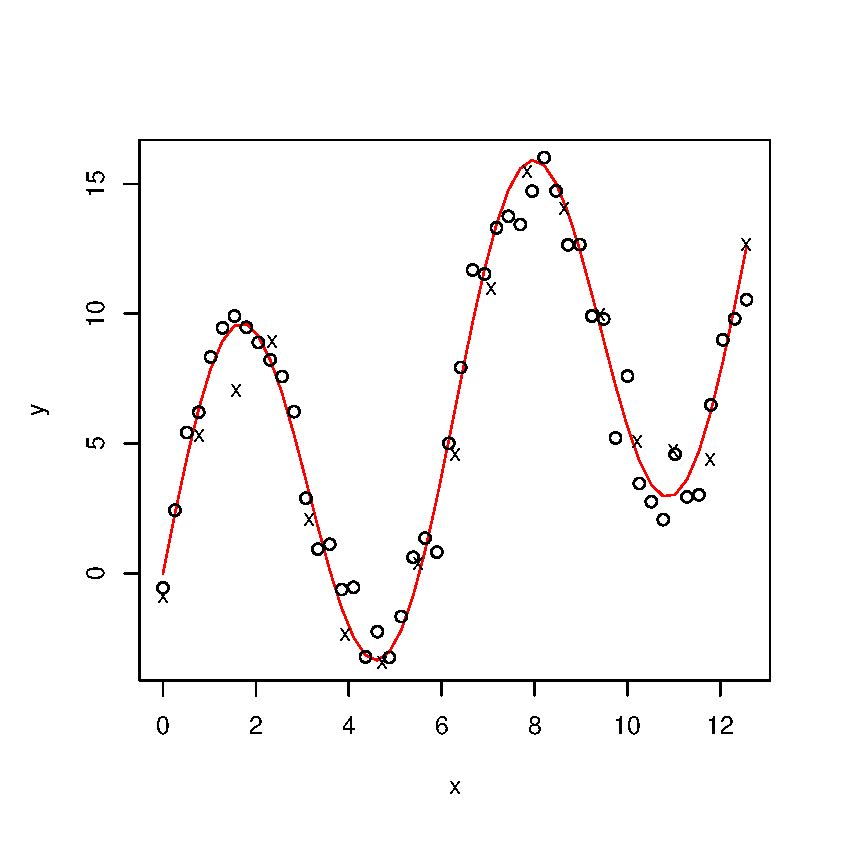
\includegraphics[height=3in]{04ANN/simpleExampleData.eps}
\end{center}
\caption{แสดงข้อมูลตัวอย่าง จุดข้อมูลสำหรับการฝึก (วงกลม) และ การทดสอบ (กากบาท); เส้นทึบแสดงฟังชั่นที่ใช้สร้างข้อมูลแต่ไม่มีสัญญาณรบกวน.}
\label{fig: ANN simple example data}
\end{figure}
%

ตัวอย่างนี้เลือกใช้โครงข่ายประสาทเทียมสองชั้น 
โดยเลือกใช้ $20$ หน่วยซ่อน และใช้ฟังชั่นกระตุ้นของเอาต์พุตเป็นฟังชั่นเอกลักษณ์ที่เหมาะสำหรับการหาค่าถดถอย.
การทำนอร์มอไลเซชั่นก็เลือกใช้วิธีที่ปรับค่าอินพุต $x$ เพื่อให้ค่าเฉลี่ยและเบี่ยงเบนมาตราฐานเป็น $0$ และ $1$ ตามลำดับ.
สำหรับการฝึกโครงข่าย ตัวอย่างนี้กำหนดค่าเริ่มต้นน้ำหนักแบบสุ่มค่า โดยค่าสุ่มจากการแจกแจงเอกรูป (uniform distribution) จากช่วงค่า $[-0.5,0.5]$.
ตัวอย่างนี้ใช้วิธีลงเกรเดียนต์ในการฝึก 
และเลือกใช้ค่าอัตราการเรียนเป็น $0.01$ และ $0.0003$ สำหรับน้ำหนักชุดซ่อนและน้ำหนักชุดเอาต์พุตตามลำดับ
โดยทำการฝึกโครงข่ายทั้งหมด $9001$ รอบ.

\begin{figure}[htp]
  \centering
  \caption{การฝึกโครงข่าย: ภาพย่อยบนซ้ายแสดงค่าผิดพลาดที่รอบฝึกต่างๆ 
  ภาพย่อยที่เหลือแสดงเอาต์พุตของหน่วยซ่อนต่างๆ (ชื่อภาพย่อย Hidden Outputs) และเอาต์พุตของโครงข่ายเปรียบเทียบกับจุดข้อมูลฝึก (ชื่อภาพย่อย Network Outputs โดย เส้นทึบแสดงเอาต์พุตของโครงข่าย และวงกลมแทนจุดข้อมูลที่ใช้ฝึก)  หลังการฝึกไป $1$, $101$, และ $301$ รอบ ตามระบุในแต่ละภาพย่อย}
  \label{fig: ANN simple example training}
  \begin{tabular}{cc}
    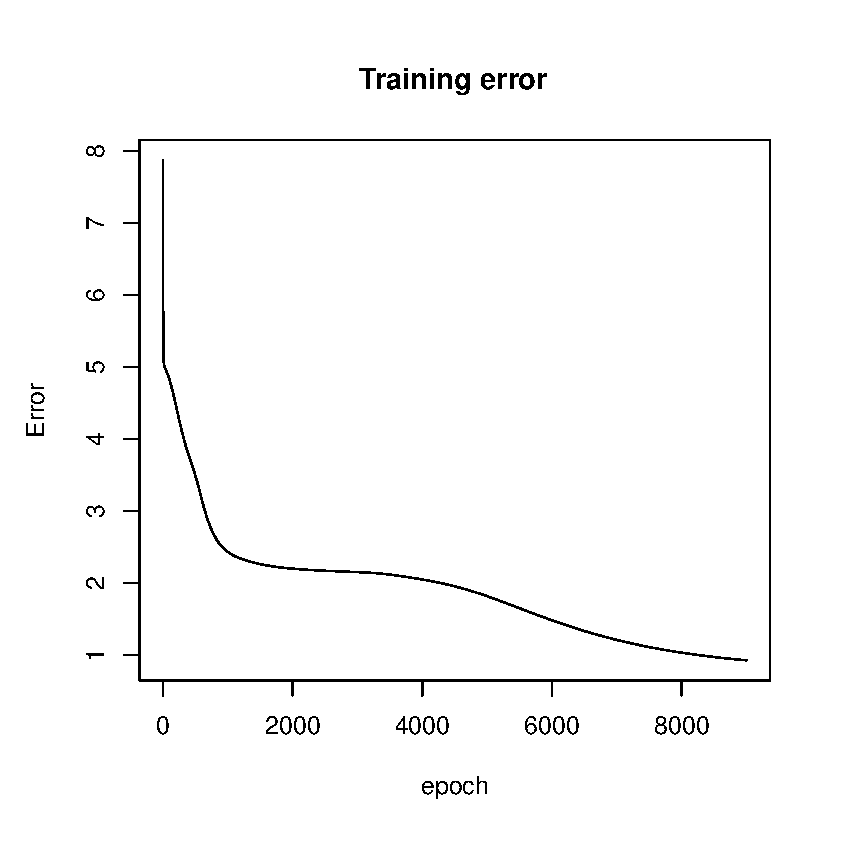
\includegraphics[width=60mm]{04ANN/error9001.eps}&    
    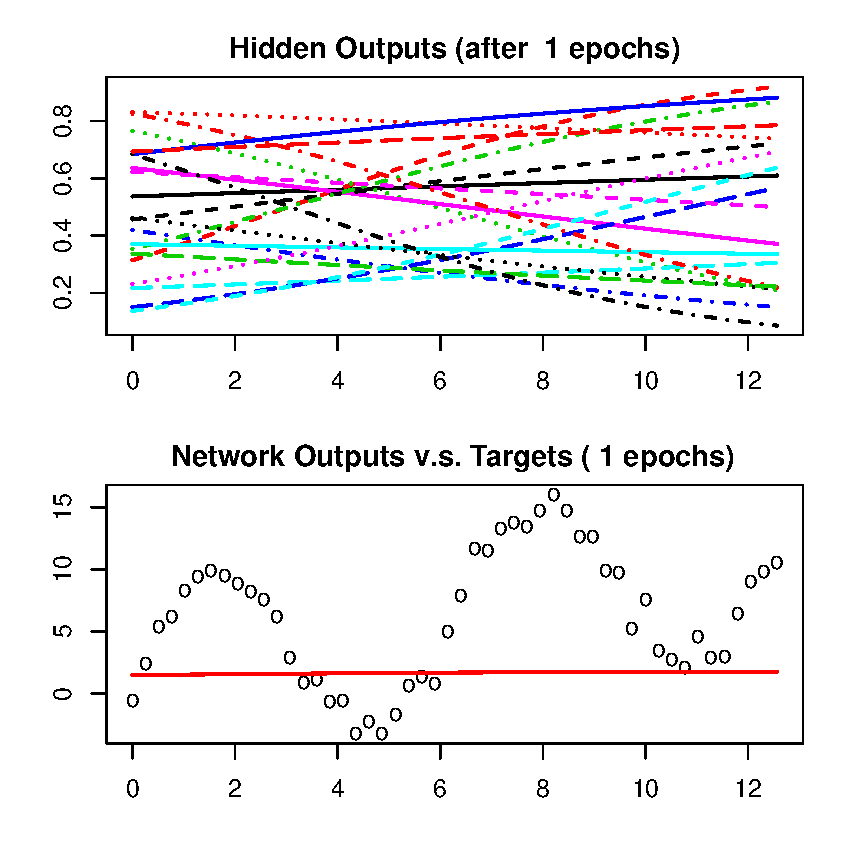
\includegraphics[width=60mm]{04ANN/simpleN1.eps}     \\
    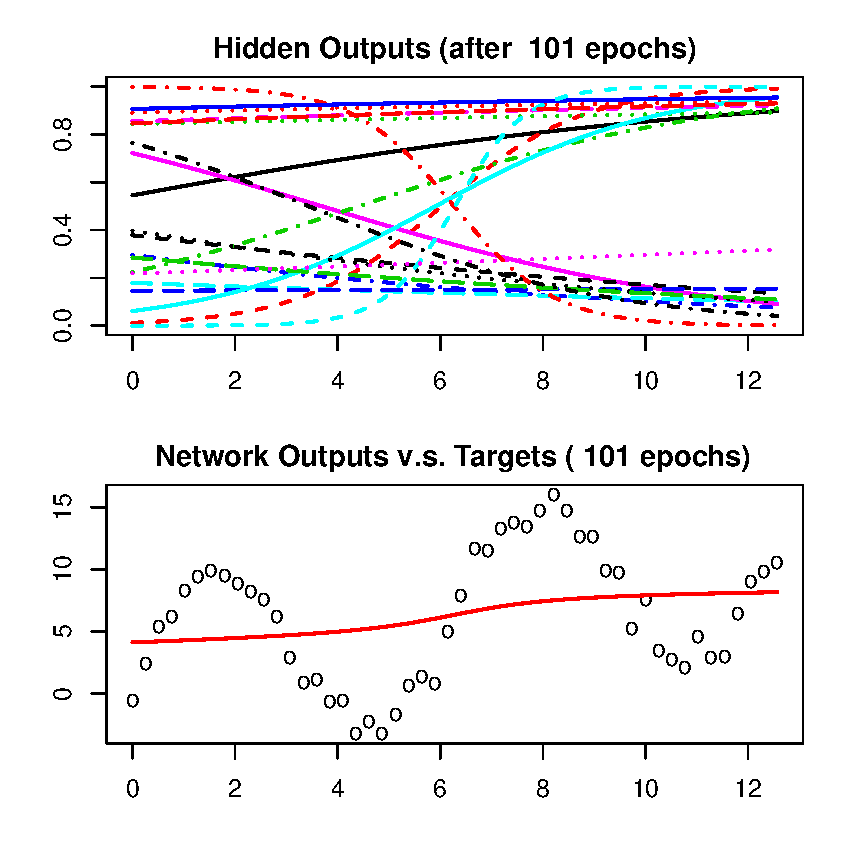
\includegraphics[width=60mm]{04ANN/simpleN101.eps}&
    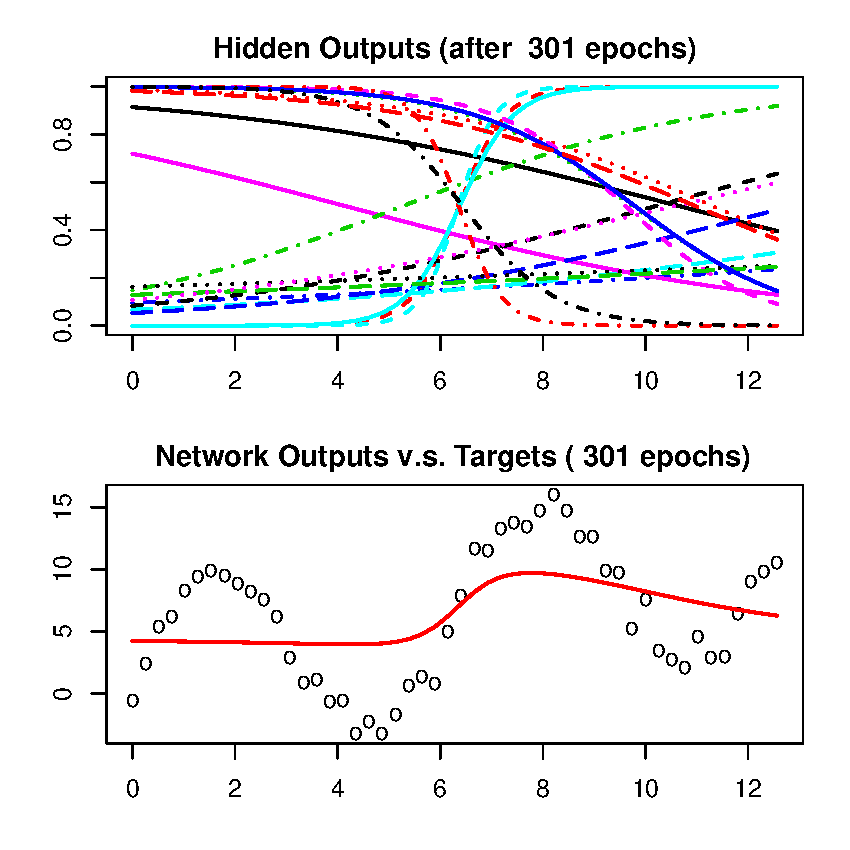
\includegraphics[width=60mm]{04ANN/simpleN301.eps}\\    
  \end{tabular}
\end{figure}

\begin{figure}[htp]
  \centering
  \caption{การฝึกโครงข่าย (ต่อ): ภาพย่อยแสดงเอาต์พุตของหน่วยซ่อนต่างๆ (ชื่อภาพย่อย Hidden Outputs) และภาพย่อยแสดงเอาต์พุตของโครงข่ายเปรียบเทียบกับจุดข้อมูลฝึก (ชื่อภาพย่อย Network Outputs โดย เส้นทึบแสดงเอาต์พุตของโครงข่าย และวงกลมแทนจุดข้อมูลที่ใช้ฝึก) หลังการฝึกไป $1001$, $3001$, $6001$ และ $9001$ ตามระบุในแต่ละภาพย่อย}
  \label{fig: ANN simple example training (continued)}
  \begin{tabular}{cc}
    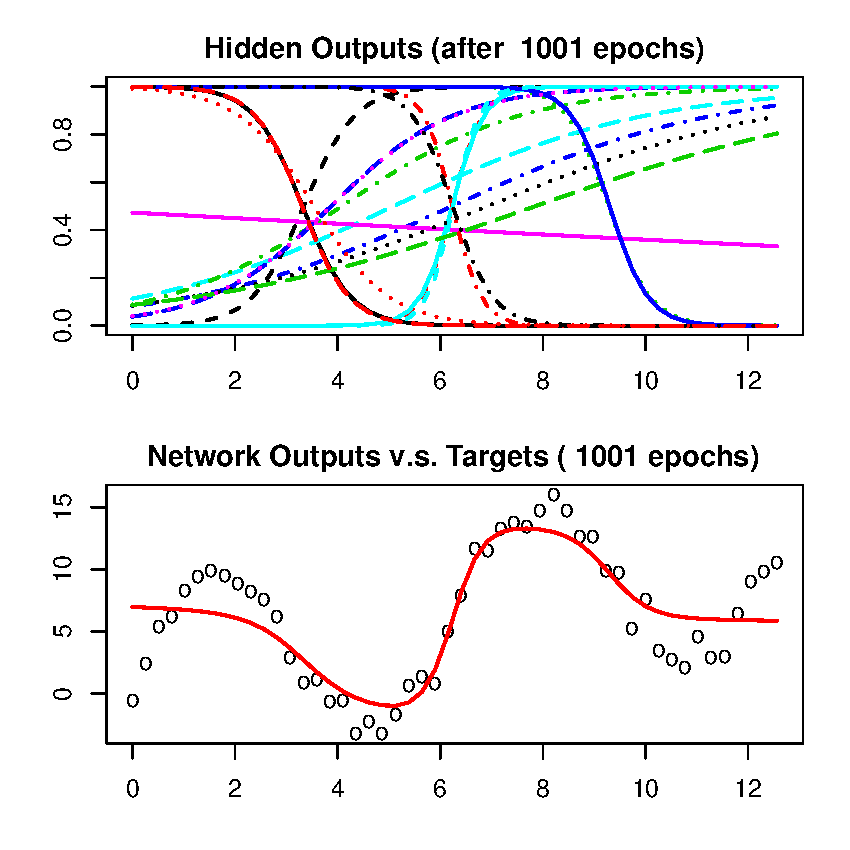
\includegraphics[width=60mm]{04ANN/simpleN1001.eps}&
    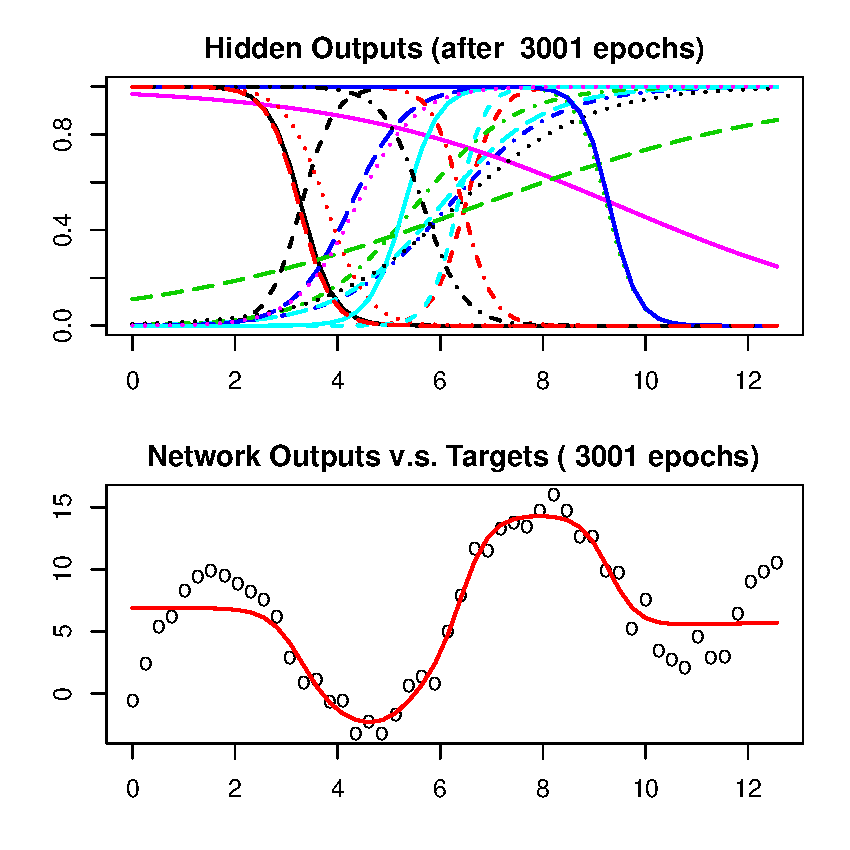
\includegraphics[width=60mm]{04ANN/simpleN3001.eps}\\
    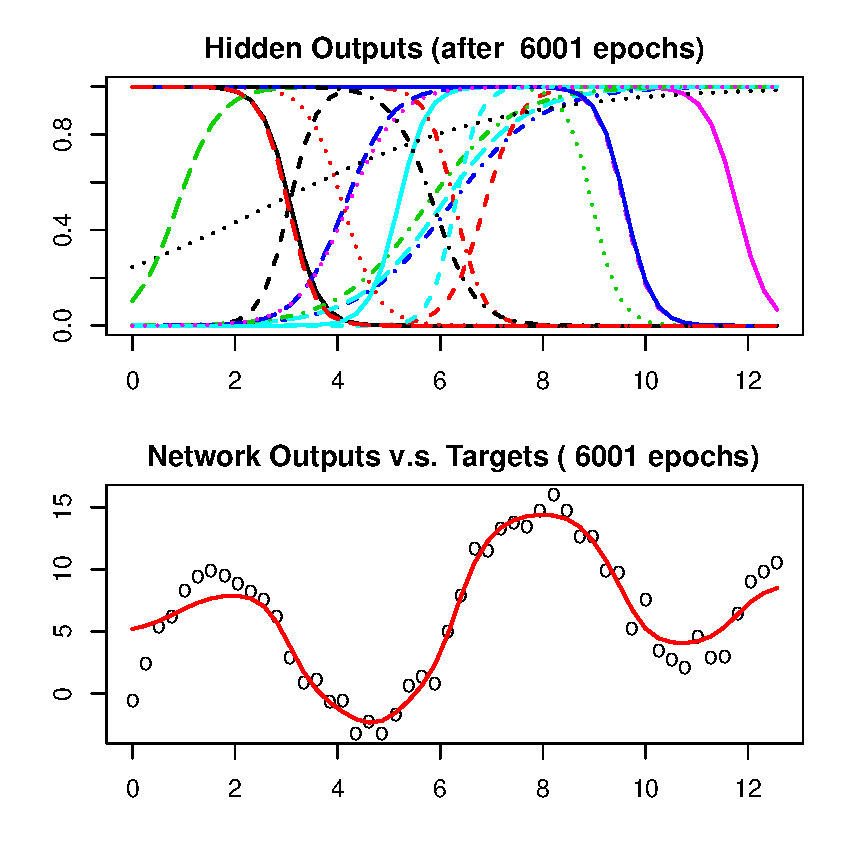
\includegraphics[width=60mm]{04ANN/simpleN6001.eps}&
    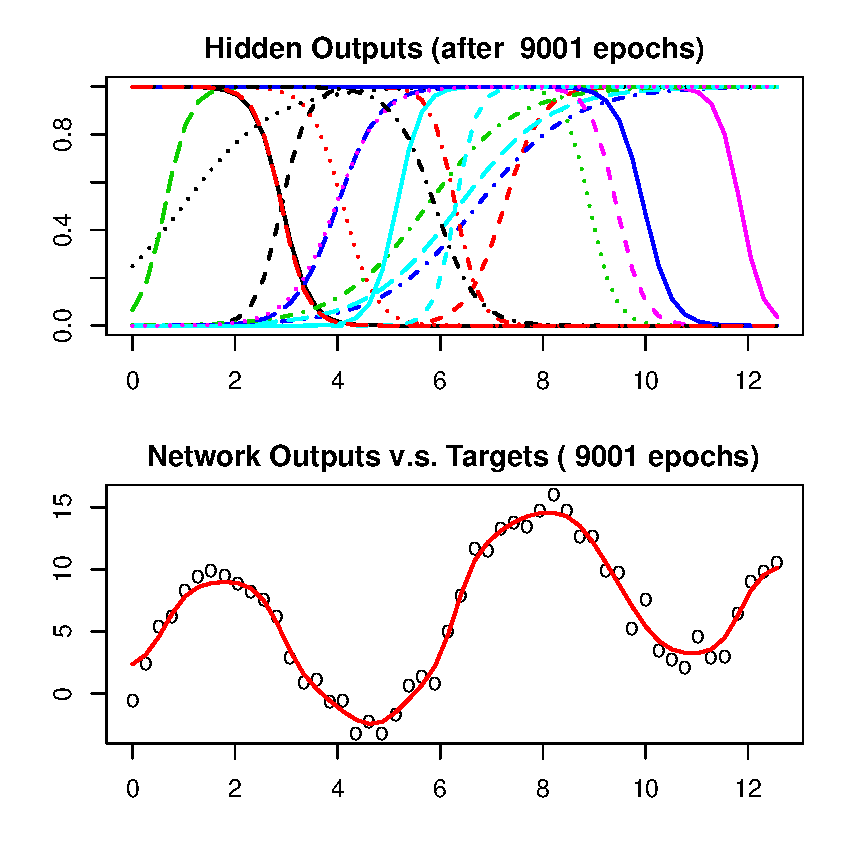
\includegraphics[width=60mm]{04ANN/simpleN9001.eps}\\
  \end{tabular}
\end{figure}

รูป~\ref{fig: ANN simple example training} แสดงค่าผิดพลาด (Root Mean Squared Error, RMSE) ที่รอบฝึก (epoch) ต่างๆ (ภาพบนซ้าย).
ค่าผิดพลาดที่แสดงนี้เป็นค่าผิดพลาดของข้อมูลชุดฝึกหัด.
ด้วยคุณสมบัติของวิธีลงเกรเดียนต์ ถ้าเราใช้ค่าอัตราการเรียนเล็กพอ 
วิธีลงเกรเดียนต์รับประกันว่า ค่าผิดพลาดนี้จะลดลงในแต่ละรอบ (หรือ อย่างน้อยก็จะไม่เพิ่มขึ้น).
หลังจากการฝึกผ่านไป $1$ รอบฝึก (ภาพบนขวา) สังเกตุว่าค่าเอาต์พุตของหน่วยซ่อนต่างๆยังมีลักษณะสุ่มอยู่มาก.
ค่าเอาต์พุตของหน่วยซ่อนจะขึ้นกับค่าอินพุต $x$ และ ค่าน้ำหนักชั้นที่หนึ่ง $\mathbf{w}^{(1)}$ เท่านั้น.
หลังจาก $1$ รอบฝึก ค่าเอาต์พุตของโครงข่ายยังมีค่าค่อนข้างคงที่ (ใกล้ๆ $0$) ตลอดช่วงค่าอินพุต $x$ (ภาพขวาที่ 2 จากบน) เพราะเรากำหนดค่าเริ่มต้นของน้ำหนักให้มีขนาดน้อยๆ.
ค่าน้ำหนักชั้นที่สองบอกส่วนผสมของเอาต์พุตของหน่วยซ่อนต่างๆ เพื่อผสมออกมาเป็นเอาต์พุตของโครงข่าย.
หลังจาก $1$ รอบฝึก เอาต์พุตต่างๆของหน่วยซ่อน มีค่าต่ำตลอดช่วงอินพุต (มีค่าอยู่ประมาณ $0.1$ ถึง $0.9$) แล้ว ค่าของน้ำหนักชั้นที่สองก็ต่ำ (เพราะเริ่มต้นด้วยค่าสุ่มจากช่วงค่าน้อยๆ และเพิ่งฝึกไปเพียงแค่ $1$ รอบ ด้วยค่าอัตราการเรียนที่น้อย) ดังนั้นค่าเอาต์พุตของโครงข่ายจึงเป็นอย่างที่เห็น ซึ่งไม่ได้ใกล้เคียงกับจุดข้อมูลฝึกที่เป็นเป้าหมายเลย.

หลังทำการฝึกไป $101$ รอบ เอาต์พุตของชั้นย่อยกระจายตัวแตกต่างกันมากขึ้น และเอาต์พุตของโครงข่ายก็เริ่มปรับตัวให้พอสังเกตุเห็นความโค้งได้บ้าง.
หลังทำการฝึกไป $301$, $1001$, $3001$ รอบ เอาต์พุตของชั้นย่อยกระจายตัวแตกต่างกันค่อนข้างชัดเจน และเอาต์พุตของโครงข่ายก็เห็นเป็นรูปร่างตามจุดข้อมูลฝึกชัดเจนขึ้น.
แต่สังเกตุว่าที่ $3001$ รอบฝึก บริเวณปลายหางของเอาต์พุตโครงข่ายยังไม่ได้ปรับตัวโค้งงอรับกับชุดข้อมูลฝึก (ประมาณบริเวณค่าแกนนอน $x > 11$) 
และเมื่อสังเกตุเอาต์พุตของชั้นซ่อนจะเห็นว่า ยังไม่มีเอาต์พุตของชั้นย่อยหน่วยใดที่มีช่วงโค้งงออยู่บริเวณนั้น.
เปรียบเทียบเอาต์พุตหลังการฝึก $3001$ รอบ กับเอาต์พุตหลังการฝึก $6001$ รอบ 
จะเห็นว่า เอาต์พุตของโครงข่ายหลังการฝึก $6001$ รอบจะมีการโค้งงอรับกับข้อมูลฝึกในช่วงปลายหาง 
และความยืดหยุ่นในการปรับตัวโค้งงอนั้น
ก็มาจากเอาต์พุตของชั้นซ้อนหน่วยหนึ่งที่ปรับตัวมาจนการเปลี่ยนพลวัตรขยับมาอยู่ช่วงดังกล่าว (เอาต์พุตของชั้นย่อยหน่วยหนึ่ง ที่แสดงด้วยเส้นทึบสีบานเย็น---เอาต์พุตของหน่วยซ้อนเส้นเด่นขวาสุดในภาพ---ได้ขยับช่วงที่เปลี่ยนค่าแนวตั้งจาก $1$ มาเป็น $0$ มาอยู่ที่บริเวณค่าแกนนอน $x \approx 11$).

หลังจากฝึกไป $9001$ รอบ ค่าน้ำหนักของโครงข่ายก็ลู่เข้า 
และเอาต์พุตของโครงข่ายก็ปรับตัวรับกับค่าของจุดข้อมูลฝึกได้ดี (ภาพขวาล่างสุด รูป~\ref{fig: ANN simple example training (continued)})
รูป~\ref{fig: ANN simple example results} แสดงผลการทดสอบของโครงข่ายที่ฝึกแล้วนี้ กับข้อมูลชุดทดสอบ.

%
\begin{figure}
\begin{center}
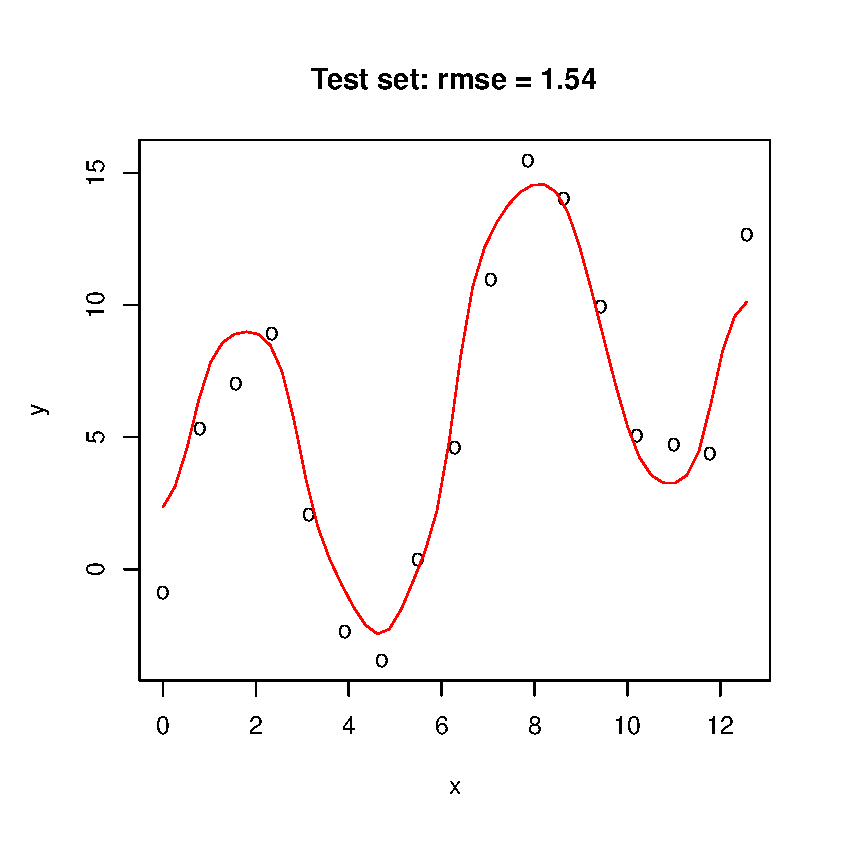
\includegraphics[height=3in]{04ANN/testResults.eps}
\end{center}
\caption{ผลการหาค่าถดถอยด้วยโครงข่ายประสาทเทียม.
กราฟเส้นทึบแสดงผลทำนายของโครงข่าย และวงกลมแสดงจุดข้อมูลทดสอบ.
ระยะห่างในแนวตั้วระหว่างวงกลมและเส้นทึบ คือค่าความผิดพลาด ซึ่งจากตัวอย่างนี้ได้ค่าความผิดพลาด RMSE เป็น $1.54$}
\label{fig: ANN simple example results}
\end{figure}
%

สังเกตุระหว่างการฝึก (รูป~\ref{fig: ANN simple example training} และ \ref{fig: ANN simple example training (continued)} หลังฝึกไป $101$, $301$, $1001$, $3001$, และ $6001$) เอาต์พุตของหน่วยซ่อนจะค่อยๆปรับตัว 
เพื่อทำให้เอาต์พุตของโครงข่ายใกล้เคียงกับข้อมูลทดสอบมากขึ้น.
นอกจากนี้ รูป~\ref{fig: ANN simple example training} และ \ref{fig: ANN simple example training (continued)} ยังเสริมมุมที่มองว่า โครงข่ายประสาทเทียมเสมือนกับโมเดลเชิงเส้นที่สามารถปรับเบซิสฟังชั่นได้.
โดยบางภาพ เช่น ภาพของเอาต์พุตของหน่วยซ่อนและโครงข่ายหลัง $6001$ รอบ เราสามารถเห็นความสัมพันธ์ระหว่างเอาต์พุตของหน่วยซ่อนและเอาต์พุตของโครงข่าย โดยเฉพาะที่อินพุตมีค่ามากกว่า $11$.
หรือ ความสัมพันธ์ระหว่างเอาต์พุตของหน่วยซ่อนและของโครงข่ายหลัง หลัง $9001$ รอบฝึก โดยเฉพาะที่อินพุตมีค่าน้อยกว่า $2$.

\section*{การหยุดก่อนกำหนด}
\label{sec: ann early stopping}
\index{early stopping}
\index{การหยุดก่อนกำหนด}

เช่นเดียวกับโมเดลทำนายอื่นๆ % เช่น การหาค่าถดถอยมิติเดียวด้วยฟังชั่นพหุนาม และการฝึกโมเดลเชิงเส้น, 
การใช้งานโครงข่ายประสาทเทียมก็ต้องคำนึงถึง เรื่อง\textit{โอเวอร์ฟิตติ้ง} (overfitting) หรือ\textit{คุณสมบัติความทั่วไป} (generalization) ด้วย.
การเลือกใช้โมเดลที่มีความยืดหยุ่นสูงๆ เช่นโครงข่ายประสาทเทียมสองชั้นที่มีจำนวนหน่วยซ่อนมากๆ ก็อาจจะเสี่ยงที่จะสูญเสียคุณสมบัติความทั่วไปได้. 
นั่นคือ แทนที่จะได้โมเดลที่สามารถประมาณระบบที่สนใจ หรือทำนายปริมาณที่สนใจได้ดี แต่ผลอาจจะเป็นการที่ได้โมเดลที่ปรับตัวไปเข้ากับสัญญาณรบกวนของข้อมูลชุดฝึกหัดแทน.
ผู้อ่านสามารถทบทวนเรื่องโอเวอร์ฟิตติ้งหรือการเสียคุณสมบัติความทั่วไปได้จากหัวข้อ~\ref{section: Polynomial Curve Fitting} และ \ref{section: Model selection}.

รูป~\ref{fig: ANN simple example overfitting} แสดงผลจากการใช้โครงข่ายขนาดหน่วยซ่อน $10$ กับ $100$ และฝึก $5,000$, $20,000$, และ $100,000$ รอบ.
สังเกตุว่า สำหรับโครงข่ายขนาดหน่วยซ่อนเป็นสิบ ($M=10$) 
การฝึกสองหมื่นรอบทำให้ได้คุณภาพของโมเดลดีขึ้น (ค่าผิดพลาดของชุดทดสอบลดลงจาก $2.12$ ที่ห้าพันรอบฝึก เหลือเพียง $1.44$ ที่สองหมื่นรอบฝึก).
แต่การฝึกต่อไปถึงหนึ่งแสนรอบฝึก แม้จะทำให้ค่าผิดพลาดของชุดฝึกต่ำลง (จาก $0.8$ ที่สองหมื่นรอบฝึก เป็น $0.75$ ที่หนึ่งแสนรอบฝึก) แต่ค่าผิดพลาดของชุดทดสอบกลับเพิ่มขึ้น (จาก $1.44$ ที่สองหมื่นรอบฝึก เป็น $1.53$ ที่หนึ่งแสนรอบฝึก).
เช่นเดียวกัน โครงข่ายขนาดหน่วยซ่อนหนึ่งร้อย ($M=100$) ที่หนึ่งแสนรอบฝึก ที่ผลลัพธ์แสดงการที่โมเดลพยายามปรับตัวไปประมาณสัญญาณรบกวนของชุดฝึกอย่างเห็นได้ชัด.
สิ่งบ่งชี้ที่สำคัญ คือ ค่าผิดพลาดของชุดฝึกที่ลดลง ในขณะที่ค่าผิดพลาดของชุดทดสอบเพิ่มขึ้น.
นี่คือการที่โมเดลปรับตัวไปประมาณสัญญาณรบกวนที่เห็นในชุดฝึก แทนที่จะประมาณระบบที่สนใจ.
พูดอีกอย่างคือ โมเดลเสียคุณสมบัติความทั่วไป หรือเกิดโอเวอร์ฟิตติ้งขึ้นนั่นเอง.

\begin{figure}[htp]
  \centering
  \caption{ผลจากโครงข่ายขนาดหน่วยซ่อนสิบหน่วย ($M=10$) กับหนึ่งร้อยหน่วย ($M=100$) ที่การฝึกผ่าน
  %ห้าพันรอบ สองหมื่นรอบ และหนึ่งแสนรอบ  
  $5000$, $20000$, และ $100000$ รอบ
  โดย แกนนอนแสดงค่าอินพุต แกนตั้งแสดงค่าเอาต์พุต
  เส้นทึบสีแดงแสดงเอาต์พุตของโครงข่าย
  กากบาทแทนจุดข้อมูลฝึก 
  และวงกลมแทนจุดข้อมูลทดสอบ}
  \label{fig: ANN simple example overfitting}

  \begin{tabular}{cc}
    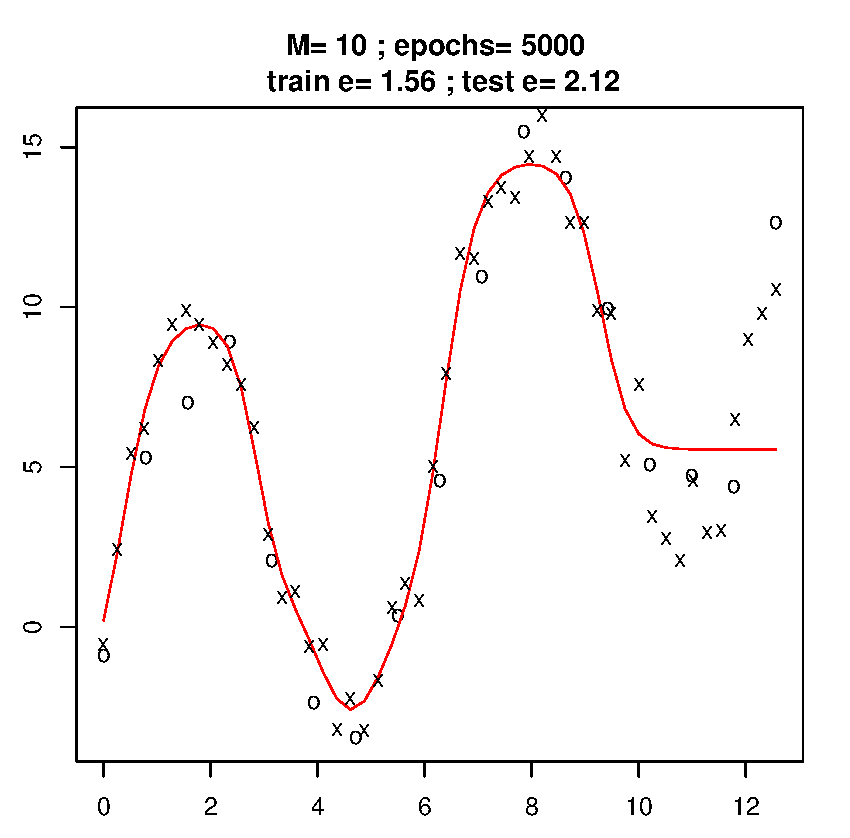
\includegraphics[width=60mm]{04ANN/simpleM10E5000.eps}&    
    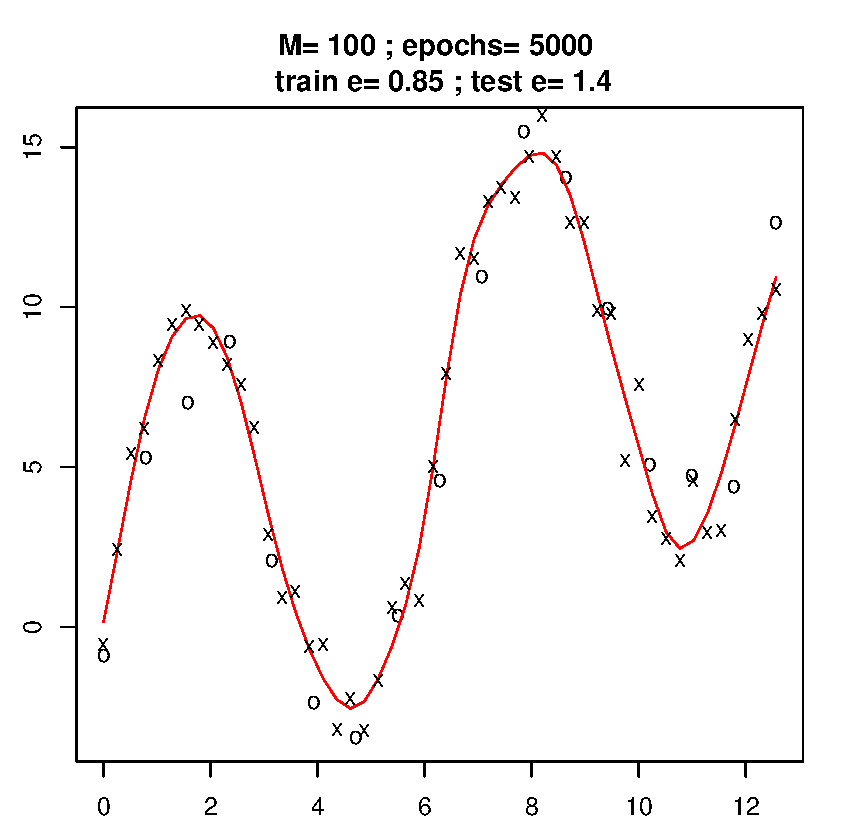
\includegraphics[width=60mm]{04ANN/simpleM100E5000.eps}     \\
    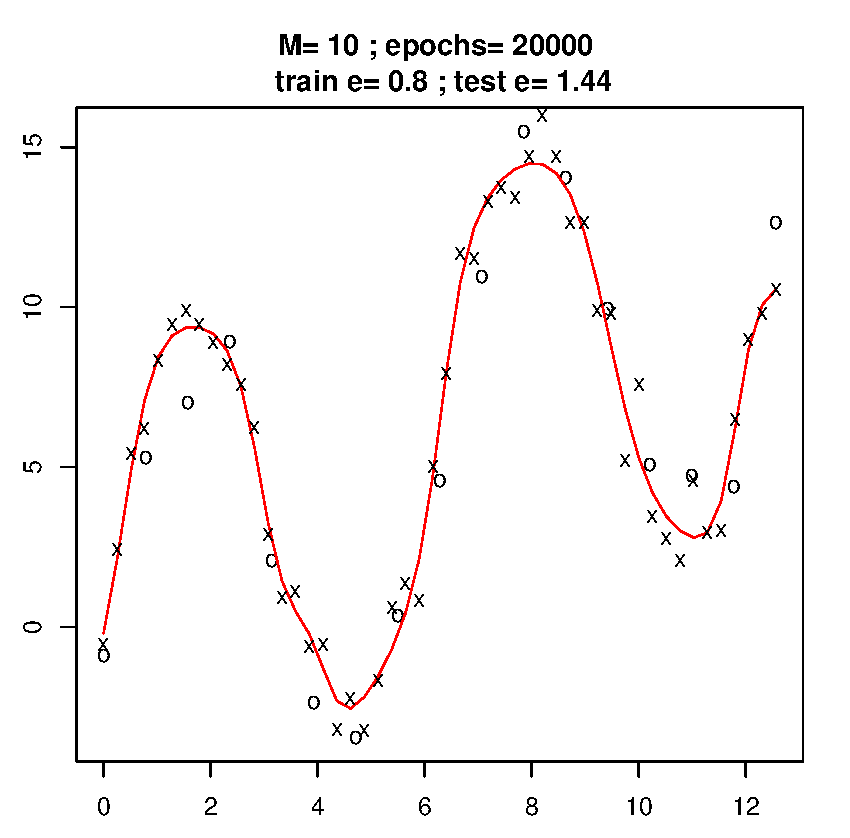
\includegraphics[width=60mm]{04ANN/simpleM10E20000.eps}    &    
    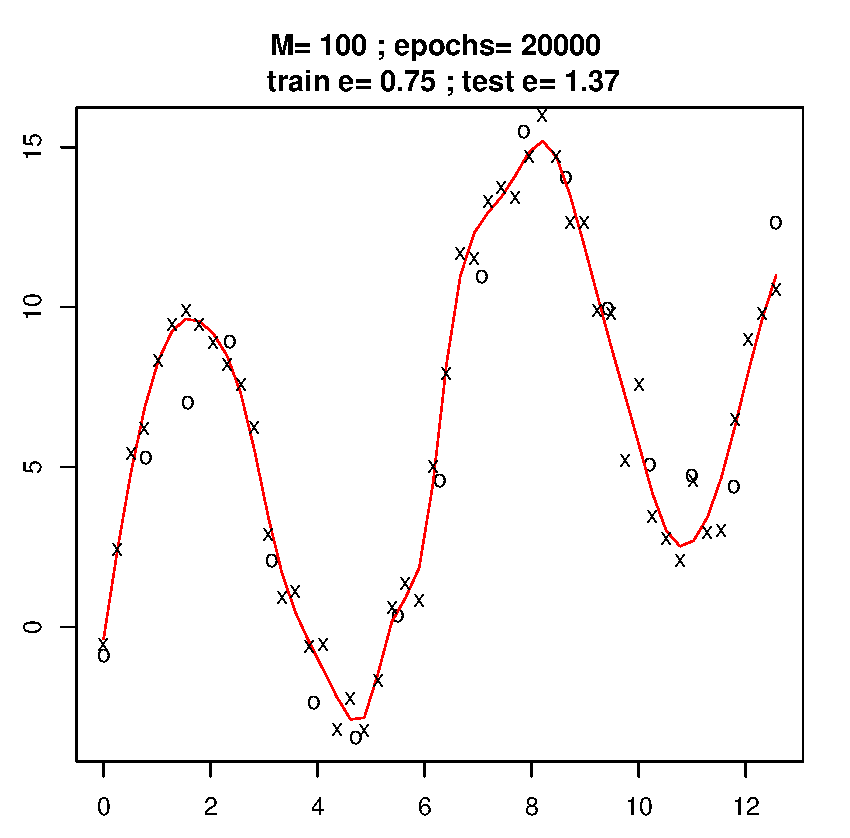
\includegraphics[width=60mm]{04ANN/simpleM100E20000.eps}     \\
    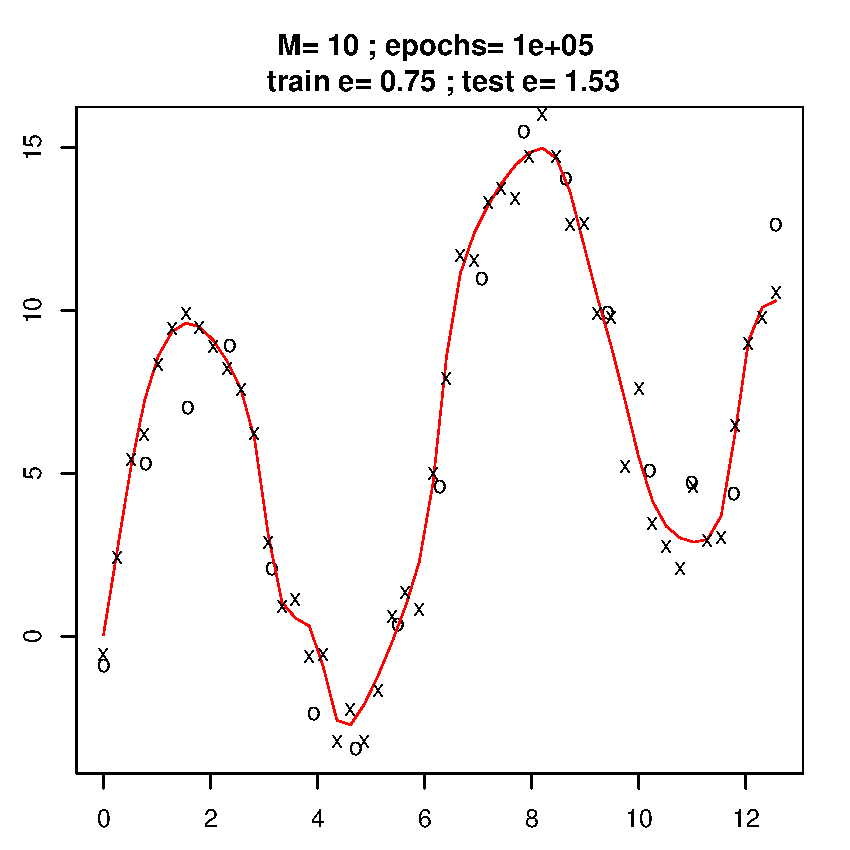
\includegraphics[width=60mm]{04ANN/simpleM10E100000.eps}&    
    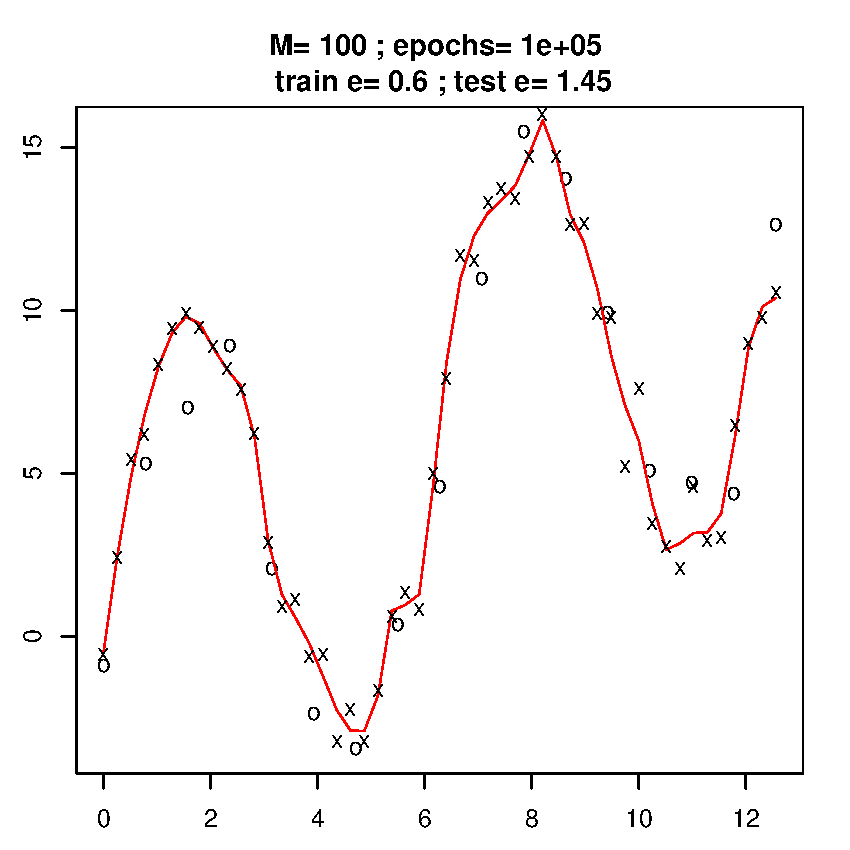
\includegraphics[width=60mm]{04ANN/simpleM100E100000.eps}           
  \end{tabular}
\end{figure}

เรื่องนี้ นอกจากทำให้ได้โมเดลทำนายที่คุณภาพต่ำแล้ว ยังทำให้เสียเวลาในการฝึกโครงข่ายเพิ่มขึ้นด้วย.
วิธีหนึ่งที่นิยมใช้กับการฝึกโครงข่ายประสาทเทียมเพื่อลดปัญหานี้คือ\textit{การทำหยุดก่อนกำหนด} (Early Stopping).

การทำหยุดก่อนกำหนดนั้นตรงไปตรงมาตามธรรมชาติของคุณสมบัติความทั่วไป.
สัญญาณบ่งชี้ว่าโมเดลเริ่มเกิดโอเวอร์ฟิตติ้งคือการที่โมเดลทำนายค่าข้อมูลชุดฝึกได้ดีขึ้น 
แต่ทำนายข้อมูลอื่น (จากระบบเดียวกัน)ได้แย่ลง.
ดังนั้น นอกจากชุดทดสอบ (ที่แยกเก็บไว้ทดสอบตอนสุดท้ายแล้ว) วิธีหยุดก่อนกำหนดจะแบ่งข้อมูลออกอีกส่วนเป็น  \textit{ชุดวาลิเดชั่น} (Validation Set) ซึ่งเป็นเสมือนชุดข้อมูลทดสอบระหว่างการทำโมเดล.
แล้วระหว่างการฝึกโครงข่าย ก็คอยตรวจสอบค่าผิดพลาดของการทำนายกับชุดข้อมูลวาลิเดชั่นนี้ ถ้าค่าผิดพลาดของชุดวาลิเดชั่นมีค่าเพิ่มขึ้น ก็เป็นสัญญาณบอกว่าอาจเกิดโอเวอร์ฟิตติ้งขึ้น.
สัญญาณนี้สามารถใช้เป็นเครื่องมือช่วยในการตัดสินใจที่จะหยุดการฝึกได้.

\section{ตัวอย่างการหาค่าถดถอย}

%
\begin{figure}
\begin{center}
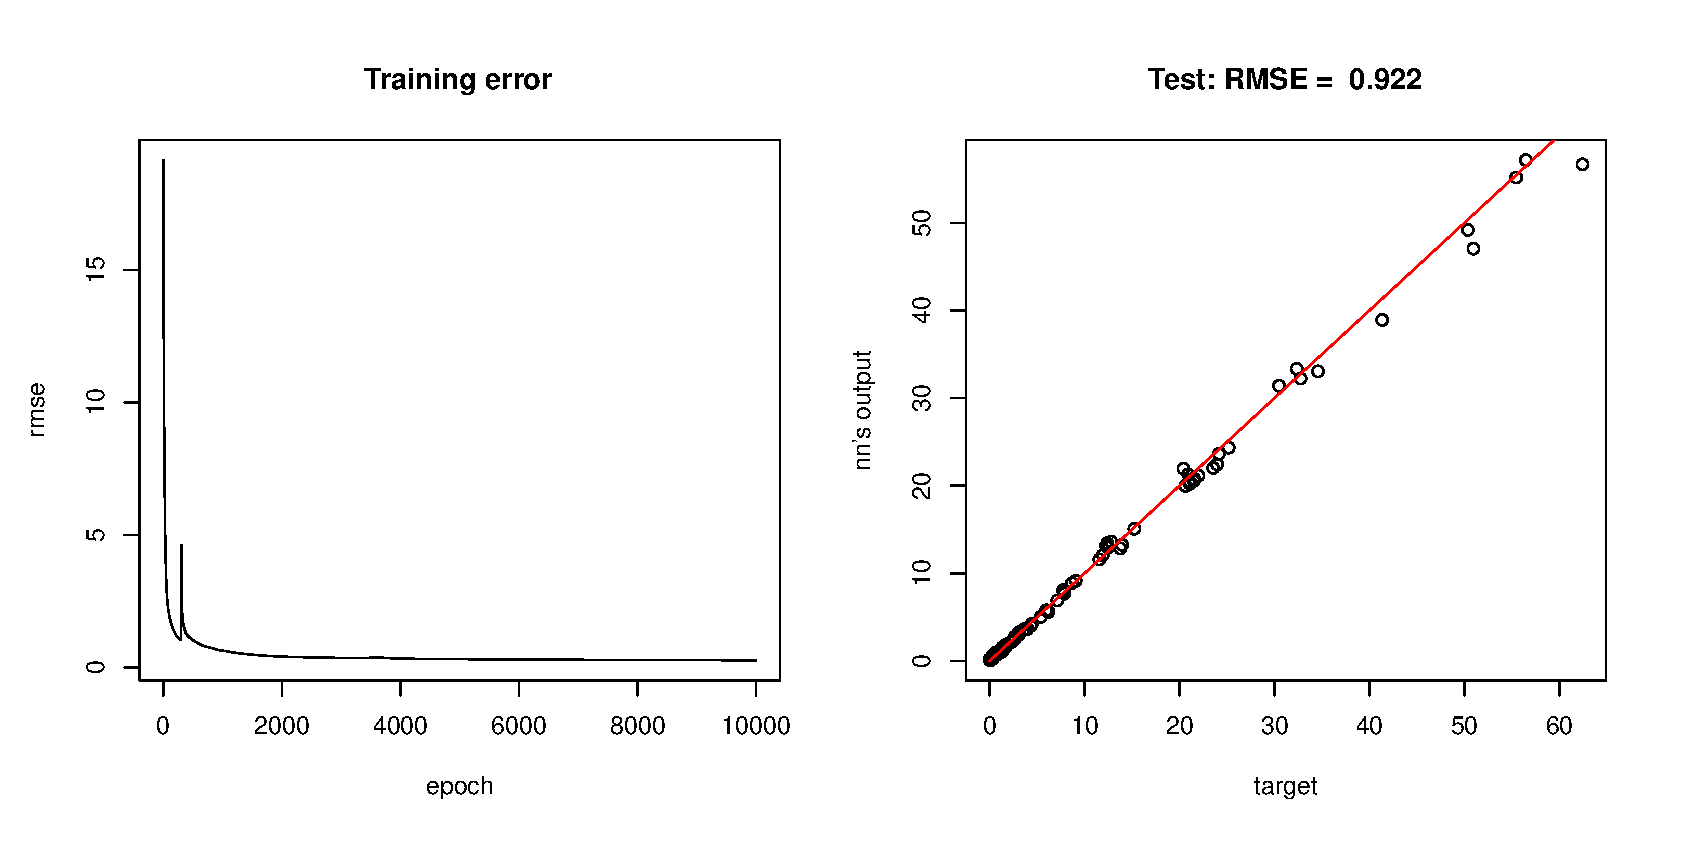
\includegraphics[height=3in]{04ANN/yachtExample.eps}
\end{center}
\caption{การฝึกและผลทดสอบการหาค่าถดถอยของข้อมูลชุดเรือยอชท์ (yacht dataset) ด้วยโครงข่ายประสาทเทียม.}
\label{fig: ANN regression example}
\end{figure}
%

หัวข้อนี้แสดงตัวอย่างการประมาณค่าแรงต้านที่เหลือค้าง (residuary resistance) ของเรือยอชต์ขณะแล่นอยู่ 
ซึ่งก็เป็นปัญหาการหาค่าถดถอย.
ข้อมูลชุดนี้ได้มาจากฐานข้อมูลของ\textit{คลังข้อมูลยูซีไอ}\cite{Bache+Lichman:2013} ที่
\url{http://archive.ics.uci.edu/ml/datasets/Yacht+Hydrodynamics}. 

ข้อมูลชุดนี้มี $308$ ระเบียน นั่นคือ มี $308$ จุดข้อมูล และแต่ละจุดข้อมูลจะมี $7$ เขตข้อมูล (7 มิติ).
เขตข้อมูลที่ 1-6 ซึ่งได้แก่ 
ตำแหน่งตามแนวยาวเรือของศูนย์กลางการลอยตัว (longitudinal position of the center of buoyancy เป็นลักษณะที่ช่วยอธิบายการกระจายน้ำหนักของเรือตามแนวยาวว่าอยู่หน้าลำ กลางลำ หรือท้ายลำอย่างไร),
ค่าสัมประสิทธิปริซึ่ม (prismatic coefficient เป็นลักษณะที่ช่วยอธิบายรูปทรงของท้องเรือ 
โดยวัดจากอัตราส่วนของปริมาตรที่อยู่ใต้น้ำของท้องเรือ 
เปรียบเทียบกับปริมาตรของรูปทรงปริซึ่มที่มีความยาวเท่ากัน 
และพื้นที่หน้าตัดเท่ากับ พื้นที่หน้าตัดที่กว้างที่สุดของท้องเรือ), 
อัตราส่วนความยาวเรือกับการกระจัด (length-displacement ratio เป็นลักษณะที่ช่วยบ่งชี้ถึงความหนักของเรือเทียบกับความยาว เรือที่หนักจะมีค่านี้มาก เรือที่เบาจะมีค่านี้น้อย), 
อัตราส่วนความกว้างเรือกับระดับจมน้ำ (beam-draught ratio เป็นลักษณะทรงท้องเรือที่วัดจาก อัตราส่วนความกว้างเรือกับความกว้างของส่วนที่กว้างที่สุดของเรือในแนวระดับน้ำ), 
อัตราส่วนความยาวกับความกว้างเรือ (length-beam ratio), 
และตัวเลขฟรูด (Froude number เป็นค่าที่บอกความต้านทานของการที่วัตถุเคลื่อนที่ในน้ำ).
เขตข้อมูลทั้งหกนี้บรรยายลักษณะรูปร่างและการกระจายน้ำหนักของท้องเรือ และเขตข้อมูลนี้จะใช้เป็นอินพุตของโมเดล.

เขตข้อมูลที่ 7 (Residuary resistance per unit weight of displacement) เป็นค่าความต้านทานเหลือค้าง ซึ่งเป็นแรงต้านสำคัญที่เกิดกับเรือ และเกี่ยวพันกับลักษณะต่างๆของเรือ ที่วัดเป็นคุณสมบัติและแสดงในเขตข้อมูลที่ 1-6. 
การประมาณค่าความต้านทานเหลือค้างนี้ได้ดีจะช่วยอย่างมากในการประเมินสมถนะของเรือ 
รวมถึงช่วยเป็นข้อมูลประกอบสำหรับการออกแบบเรือด้วย เช่น การเลือกรูปทรงและขนาดของท้องเรือ การกำหนดน้ำหนักบรรทุกของเรือ การเลือกขนาดของเครื่องยนต์ที่เหมาะสม เป็นต้น.
(ดูคำอธิบายเพิ่มเติมจาก\textit{คลังข้อมูลยูซีไอ} และอรทิโกสาและคณะ\cite{OrtigosaEtAl2007a})

จากข้อมูล $308$ จุด เราแบ่งข้อมูล $215$ จุด ($70\%$) เป็นข้อมูลชุดฝึก และใช้ที่เหลือสำหรับการทดสอบ.
เราใช้โครงข่ายขนาด $10$ หน่วยย่อยในการทำการหาค่าถดถอยนี้.
รูป~\ref{fig: ANN regression example} แสดงค่าผิดพลาดระหว่างการฝึกและผลการทดสอบ.
ผลการทดสอบในภาพขวามือแสดงให้เห็นว่าโครงข่ายประสาทเทียมที่ฝึกแล้วทำงานได้ดีพอสมควร
ดังเห็นได้จากที่ความผิดพลาด (RMSE) ของชุดทดสอบมีค่าต่ำ และค่าเอาต์พุตจากโครงข่ายใกล้กับค่าจริงมาก (ผลการวาดค่าเอาต์พุตจากโครงข่ายกับค่าจริงเรียงตัวเกือบทับเส้นตรง $y = x$).

สังเกตุว่า ค่าผิดพลาดระหว่างการฝึก (ภาพซ้ายมือ) บางครั้งกลับมีค่าเพิ่มขึ้นได้.
ที่เป็นเช่นนี้ก็เพราะว่า ค่าอัตราการเรียนรู้ที่เลือกใช้อาจมีค่าสูงเกินไปเล็กน้อย (\texttt{rhoh=0.001}, \texttt{rhoo=0.0003}, ดูหัวข้อ~\ref{sec: regression example code}).
แต่เนื่องจากการฝึกสามารถดำเนินต่อไปได้ (ดูจากค่าผิดพลาดที่หลังจากนั้นก็ลดลงอย่างต่อเนื่อง)
ค่าอัตราการเรียนรู้ชุดนี้ก็ถือว่าใช้ได้ (ค่าอัตราการเรียนรู้ไม่มากเกินไปจนทำให้วิธีลงชันที่สุดล้มเหลว)

ตัวอย่างนี้เลือกใช้ค่าอัตราการเรียนรู้ให้เป็นค่าคงที่ตลอดการฝึก.
การเลือกค่าน้อยๆอาจช่วยให้ค่าผิดพลาดลดลงต่อเนื่องอย่างดี (ค่าพารามิเตอร์ลู่เข้าค่าทำน้อยที่สุดท้องถิ่น) แต่ก็อาจต้องเพิ่มจำนวนรอบฝึกเพื่อชดเชย (ส่งผลโดยอ้อมทำให้ฝึกเสร็จช้าลง).
การเลือกใช้ค่าอัตราการเรียนรู้ค่าใหญ่ขึ้นทำให้ต้องการรอบฝึกน้อยลง (ส่งผลโดยอ้อมให้ฝึกเสร็จเร็วขึ้น)
แต่หากใช้ค่าอัตราการเรียนรู้ค่าใหญ่เกินไปจะทำให้ค่าพารามิเตอร์ไม่ลู่เข้า และทำให้การฝึกไม่มีเสถียรภาพและ อาจจะทำให้ผลการฝึกล้มเหลวได้.

ในการประยุกต์ใช้งานโครงข่ายประสาทเทียม ผู้ใช้ต้องตรวจสอบกระบวนการฝึก เช่น ตรวจสอบดูค่าผิดพลาดต่อรอบฝึก ดังภาพซ้ายในรูป~\ref{fig: ANN regression example} เพื่อตรวจดูว่าการฝึกเป็นไปด้วยดี.
หากค่าผิดพลาดเพิ่มขึ้นเรื่อยๆ หรือมีการเปลี่ยนแปลงค่ารุนแรงมาก นั้นอาจเป็นสัญญาณว่าอัตราการเรียนรู้มีค่ามากเกินไป.
แต่หากแนวโน้มของค่าผิดพลาดยังลดลงอยู่เมื่อครบจำนวนรอบฝึกแล้ว นั่นอาจบ่งบอกถึงการควรลองเพิ่มจำนวนรอบฝึกดู.
ค่าผิดพลาดต่อรอบฝึกของภาพซ้ายในรูป~\ref{fig: ANN regression example} มีลักษณะราบตอนปลายๆ (ค่าผิดพลาดไม่ค่อยลดลงอีก) แสดงถึงว่าจำนวนรอบฝึกน่าจะเพียงพอแล้ว.

เรื่องค่าอัตราการเรียนรู้นั้น ไม่จำเป็นที่ต้องเลือกใช้อัตราการเรียนรู้ที่มีค่าคงที่ตลอดการฝึก.
การฝึกโครงข่ายอาจทำโดยเลือกใช้อัตราการเรียนรู้ที่มีค่าสูงๆในตอนต้นๆ และปรับค่าลดลงเมื่อฝึกไปสักพักแล้วก็ได้
นอกจากนั้น การปรับค่าอัตราการเรียนรู้ตามผลการทำงานของโมเดลก็สามารถทำได้.
%หัวข้อ~\ref{sec: ann advanced optimization} กล่าวถึง
วิธีที่เลือกมาฝึกโมเดลก็จะเกี่ยวพันโดยตรงกับค่าอัตราการเรียนรู้ เพราะค่าอัตราการเรียนรู้สำหรับการฝึกโครงข่ายประสาทเทียมก็คือค่าขนาดก้าว (step size) ของ วิธีลงเกรเดียนต์ที่เลือกใช้นั่นเอง.

ดังที่อภิปรายไปแล้วว่า การฝึกโครงข่ายก็คือการหาค่าน้ำหนักที่ทำให้ฟังชั่นเป้าหมายมีค่าน้อยที่สุด.
ดังนั้น วิธีการหาค่าน้อยที่สุดที่มีประสิทธิภาพต่างๆ เช่น \textit{บีเอฟจีเอส} (BFGS) หรือ \textit{คอนจูเกตเกรเดียนต์} (Conjugate Gradient) ก็สามารถนำมาใช้ในการฝึกโครงข่ายได้.
นอกจากนั้น ยังมีวิธีที่ออกแบบมาเฉพาะสำหรับฝึกโครงข่ายและมีประสิทธิภาพมากกว่าวิธีลงเกรเดียนต์อยู่หลายวิธี เช่น 
\textit{วิธีเลเวนเบิร์กมาร์คอร์ต} (Levenberg Marquardt\cite{HaganMenhaj1994a}), \textit{เรซิเลียนต์แบกพรอพาเกชั่น} (Resilient Backpropagation, คำย่อ RPROP\cite{RiedmillerBraun1993a}), และ \textit{สเกลคอนจูเกตเกรเดียนต์} (Scaled Conjugate Gradient, คำย่อ SCG\cite{Moller1993a}) เป็นต้น.
หัวข้อ~\ref{sec: BFGS example} และ~\ref{sec: scg example} แสดงตัวอย่างการใช้วิธีบีเอฟจีเอสและสเกลคอนจูเกตเกรเดียนต์ในการฝึกโครงข่าย.

\section{ตัวอย่างการจำแนกประเภท}
\label{sec: ann biclass example}

หัวข้อนี้แสดงตัวอย่างการจำแนกประเภท ด้วยข้อมูลชุดภาพเอ็กซเรย์เต้านมของมวลเนื้อ (Mammographic Mass) 
จาก\textit{คลังข้อมูลยูซีไอ}ที่ \url{http://archive.ics.uci.edu/ml/datasets/Mammographic+Mass}.
ข้อมูลชุดนี้ 
เอลเตอร์และคณะ\cite{ElterEtAl2007a}ใช้ศึกษาการทำนายผลการตรวจภาพเอ็กซเรย์เต้านมของร่องรอยมวลเนื้อ (mammographic mass lesion) ว่าเป็น\textit{เนื้อดี} (benign) หรือ\textit{เนื้อร้าย} (malignant) จากค่าไบแรตส์ (BI-RADS) และอายุของผู้ป่วย.
%จากคำอธิบายของชุดข้อมูล 
\textit{วิธีตรวจภาพเอ็กซเรย์เต้านม} (Mammography) เป็นวิธีที่มีประสิทธิผลมากที่สุดในการตรวจมะเร็งทรวงอก \cite{ElterEtAl2007a}.
ข้อมูลชุดนี้ประกอบด้วย ค่าการประเมินไบแรตส์ (BI-RADS assessment ที่มีค่าในช่วง $\{1, 2, 3, \ldots, 5 \}$), 
อายุของผู้ป่วย (เลขจำนวนเต็มของอายุ หน่วยเป็นปี), 
รูปทรงของมวลเนื้อ (mass shape ซึ่งถูกแทนด้วย 
1 สำหรับทรงกลม round, 
2 สำหรับทรงรี oval, 
3 สำหรับทรงกลีบย่อย lobular, 
4 สำหรับทรงที่ผิดแปลก irregular), 
ลักษณะขอบของมวลเนื้อ (mass margin ซึ่งถูกแทนด้วย
1 สำหรับเขตรอบชัดเจน circumscribed, 
2 สำหรับขอบเขตเป็นกลีบย่อยๆ microlobulated, 
3 สำหรับขอบเขตคลุมเครือ obscured, 
4 สำหรับขอบเขตยากจะระบุ ill-defined, 
5 สำหรับขอบเขตเป็นลักษณะหนามหรือปุ่ม spiculated),
ความหนาแน่นของมวลเนื้อ (mass density ซึ่งถูกแทนด้วย
1 สำหรับความหนาแน่นสูง high, 
2 สำหรับความหนาแน่นกลางๆ iso, 
3 สำหรับความหนาแน่นต่ำ low, 
4 สำหรับมวลเนื้อมีไขมันอยู่ fat-containing),
และความร้ายแรง (severity ซึ่งมีสองค่า
0 สำหรับ\textit{เนื้อดี} benign
หรือ 1 สำหรับ\textit{เนื้อร้าย} malignant).
ค่า\textit{ความร้ายแรง}คือค่าที่ต้องการทำนาย (ว่าเป็น\textit{เนื้อดี}หรือ\textit{เนื้อร้าย}).
การสามารถทำนายค่า\textit{ความร้ายแรง}ได้อย่างแม่นยำจะช่วยให้แพทย์สามารถตัดสินใจได้ดีขึ้นว่า 
ควรจะทำการตัดเนื้อจากบริเวณที่สงสัยออกตรวจเพื่อยืนยันผลหรือไม่.

{\small
\begin{shaded}
กระบวนการรักษามะเร็งเป็นกระบวนการที่มีผลกระทบมาก เช่น 
นอกเหนือไปจากความเสี่ยงอื่นๆ
ผู้รับการรักษาจะเจ็บปวดทรมานจากกระบวนการรักษาเองด้วย.
ดังนั้นการวินิจฉัยผู้เข้ารับกระบวนการรักษามะเร็งจึงมีความสำคัญมาก
ที่จะระบุผู้ที่ต้องการรับการรักษาอย่างถูกต้อง
และผลกระทบจากการระบุผิดพลาดมีผลเสียหายมากทั้งสองทางไม่ว่า
ระบุผิดว่าผู้ตรวจเป็นมะเร็งโดยที่ไม่ได้เป็น (false positive)
หรือระบุผิดว่าผู้ตรวจไม่ได้เป็นโดยที่ผู้ตรวจเป็น (false negative).

การตรวจที่ผลการตรวจน่าเชื่อถือมากที่สุดคือการตัดเนื้อออกตรวจ (biopsy).
แต่การทำการตัดเนื้อออกตรวจ ผู้ตรวจต้องเข้ารับการผ่าตัด.
ซึ่งจุดประสงค์ของการทำวินิจฉัยเบื้องต้นด้วยภาพเอ็กซเรย์เต้านมของมวลเนื้อ
ก็เพื่อลดการทำการตัดเนื้อออกตรวจที่ไม่จำเป็นลงไป.
หาก\textit{การวินิจฉัยเบื้องต้นด้วยภาพเอ็กซเรย์เต้านมของมวลเนื้อ}สามารถให้ผลที่เชื่อถือได้
ผู้ตรวจที่ผลเบื้องต้นออกเป็นเนื้อดี ก็จะได้เพียงแต่สังเกตุอาการ โดยไม่จำเป็นต้องเข้าทำการตัดเนื้ออกตรวจ.
\end{shaded}
}%small

% (การตัดเนื้อออกตรวจเรียกว่า biopsy) กับรอย (lesion) ที่สงสัยจาก ผล mammogram หรือ ควรจะ สังเกตุอาการระยะสั้นแทน เมื่อ ผลน่าจะเป็น benign. % (เพื่อ ที่ผู้ป่วย ที่ผลน่าจะเป็น benign จะได้ไม่ต้องทำ biopsy โดยไม่จำเป็น).
ข้อมูลชุดนี้มี $961$ ระเบียน ($961$ จุดข้อมูล),
เฉลย หรือ ผลการตรวจจริง (ground truth) มี $516$ ระเบียนที่ผลเป็นเนื้อดี และ $445$ ระเบียนที่ผลเป็นเนื้อร้าย.

ข้อมูลชุดนี้มีค่าบางค่าของเขตข้อมูลที่ไม่ครบ (missing attribute values) ได้แก่
ค่าการประเมินไบแรตส์ขาดไป $2$ ค่า, 
อายุขาดไป $5$ ค่า, 
รูปทรงของมวลเนื้อขาดไป $31$ ค่า,
ลักษณะขอบของมวลเนื้อขาดไป $48$ ค่า, 
ความหนาแน่นของมวลเนื้อขาดไป $76$ ค่า, 
ความร้ายแรงมีค่าครบทุกระเบียน.

\paragraph{การจัดการกับค่าที่ขาดไปของบางเขตข้อมูล (missing data)}
\index{How to deal with missing attribute values}
\index{การจัดการกับค่าบางเขตข้อมูลที่ไม่มี}

มีหลายวิธีที่นิยมใช้จัดการกับกรณีที่ข้อมูลมีบางระเบียนที่มีข้อมูลไม่ครบทุกเขตข้อมูล (missing data)
วิธีง่ายๆ เช่น 
(1) การตัดจุดข้อมูลที่มีค่าไม่ครบทิ้งไปเลย %(ignoring datapoints with missing attribute values)
หรือ (2) การแทนค่าข้อมูลที่ขาดหายไปด้วยค่าเฉลี่ย (สำหรับเขตข้อมูลค่าต่อเนื่อง continuous-value field) หรือแทนด้วยค่าที่พบบ่อยที่สุดในเขตข้อมูลนั้น (สำหรับเขตข้อมูลที่เป็นลักษณะฉลากของหมวดหมู่ categorical field)
หรือ (3) การแทนค่าที่หายไปด้วยทุกค่าที่เป็นไปได้ %(assigning all possible values of the attribute) 
นั่นคือจุดข้อมูลที่ค่าเขตข้อมูลหายไปจะถูกแทนด้วยจุดข้อมูลใหม่หลายๆจุด โดยที่จุดใหม่แต่ละจุดจะมีค่าเหมือนจุดเดิม ยกเว้นค่าที่หายไปแทนด้วยค่าที่เป็นไปได้ค่าหนึ่ง
ดังนั้นจำนวนจุดข้อมูลใหม่ที่เพิ่มมาแทนนี้จะเท่ากับจำนวนค่าที่เป็นไปได้ของค่าเขตข้อมูลที่หายไป.
%หรือ บางที่วิธีที่นิยม และ ทำได้ง่าย เช่น แทนค่าที่หายไป ด้วย ค่าในเขตข้อมูลนั้นที่พบบ่อยที่สุด (assigning the most common attribute value) 
การทดลองของกรึซีมาลา-บุสเสและฮู\cite{Grzymala-BusseHu2000a}พบว่า 
การแทนค่าที่หายไปด้วยค่าที่พบบ่อยที่สุดนั่น แม้เป็นวิธีที่ทำได้ง่าย แต่ไม่ใช่วิธีให้ผลที่ดีเลย.
ตัวอย่างวิธีทำในหัวข้อ~\ref{sec: ann app biclass example code} แสดงการใช้วิธีแทนค่าที่หายไปด้วยทุกค่าของเขตข้อมูล ซึ่งเป็นวิธีที่กรึซีมาลา-บุสเสและฮูแนะนำสำหรับผลการทำงาน 
แต่เป็นวิธีที่ค่อนข้างยุ่งยากในการทำ.
ดูกรึซีมาลา-บุสเสและฮู\cite{Grzymala-BusseHu2000a}เพิ่มเติม 
สำหรับวิธีต่างๆในการจัดการข้อมูลที่ขาดหายไป 
และผลการทดลองเปรียบเทียบวิธีการต่างๆ.

สังเกตุ\textit{โครงข่ายประสาทเทียมแบบจ่ายไปข้างหน้าสองชั้น}มีสิ่งที่ผู้ใช้ต้องกำหนดอยู่หลายอย่าง 
เช่น จำนวนหน่วยซ่อน, วิธีการฝึก ที่แม้จะเลือกใช้วิธีลงเกรเดียนต์แล้วก็ยังต้องเลือก ค่าอัตราการเรียนรู้ และจำนวนรอบฝึก เป็นต้น.
สิ่งต่างๆที่ต้องเลือกเหล่านี้ก็สามารถมองเป็นพารามิเตอร์ของโมเดลได้เช่นกัน
และเพื่อกันการสับสนกับค่าน้ำหนัก (ซึ่งก็เป็น พารามิเตอร์ของโมเดล) 
เราจะเรียก\textit{พารามิเตอร์}ที่เป็นเหมือนตัวกำหนดลักษณะใหญ่ของโมเดลว่า\textit{ไฮเปอร์พารามิเตอร์} (hyperparameters) \index{hyperparameters} เพื่อให้ต่างจาก\textit{พารามิเตอร์} ซึ่งใช้อ้างถึงค่าน้ำหนัก.
โดยปกติ กระบวนการคือเลือกค่าของ\textit{ไฮเปอร์พารามิเตอร์}ก่อน
แล้วจึงนำโมเดลไปฝึก เพื่อหาค่าที่ดีของ\textit{พารามิเตอร์}ของโมเดล (ซึ่งสำหรับโครงข่ายประสาทเทียมพารามิเตอร์ก็คือค่าน้ำหนัก).

เช่นเดียวกับวิธีการเลือกโมเดลที่ถกในหัวข้อ~\ref{section: Model selection}, 
วิธีครอสวาลิเดชั่น (cross-validation) สามารถนำมาช่วยในการเลือกค่า\textit{ไฮเปอร์พารามิเตอร์}เหล่านี้ได้.
วิธีครอสวาลิเดชั่นแบบสิบพับเป็นที่นิยมใช้มาก.
บางงานวิจัย เช่น บทความของแมคแคฟฟรีย์\cite{McCaffrey2013a}แนะนำว่า โดยทั่วๆไปการใช้วิธีครอสวาลิเดชั่นสิบพับเป็นตัวเลือกที่ดี.
แต่จุดประสงค์ของตัวอย่างนี้คือ เพื่อแสดงให้เห็นการนำโครงข่ายประสาทเทียมไปประยุกต์ใช้ 
และเพื่อลดเวลาในการเตรียมตัวอย่าง 
หัวข้อนี้แสดงตัวอย่างที่ใช้วิธีครอสวาลิเดชั่นแบบห้าพับ (5-fold cross-validation).
วิธีแบบสิบพับก็สามารถทำได้ในลักษณะเดียวกัน.

ทบทวนอีกครั้ง จุดประสงค์ของ\textit{วิธีครอสวาลิเดชั่น}คือเพื่อช่วยในการเลือกโมเดล หรือในกรณีนี้คือเลือกค่าของ\textit{ไฮเปอร์พารามิเตอร์}ที่จะใช้.
ค่า\textit{ไฮเปอร์พารามิเตอร์}ที่สนใจในที่นี้คือ จำนวนหน่วยซ่อน ($M$: $5$, $10$, $30$) ที่ฝึกด้วยวิธีลงเกรเดียนต์กับอัตราการเรียนรู้ ($\{\rho_1$, $\rho_2\}$: $\{0.01, 0.001\}$,
$\{0.01, 0.01\}$, $\{0.001, 0.0\}$) 
และทำการฝึก $5000$ รอบฝึกสำหรับทุกชุดของค่าไฮเปอร์พารามิเตอร์.
ดังนั้น นั่นคือเท่ากับว่ามี\textit{ไฮเปอร์พารามิเตอร์}ที่สนใจอยู่ $9$ ชุด 
แต่ละชุดจะทำการฝึกและทดสอบ $5$ ครั้ง (เนื่องจากทำ\textit{วิธีครอสวาลิเดชั่นแบบห้าพับ})
ประสิทธิภาพของ\textit{ไฮเปอร์พารามิเตอร์}แต่ละชุดจะได้จากการเฉลี่ยค่าความแม่นยำ\footnote{บ่อยครั้ง ที่ผลมักจะแสดงออกมาในรูป\textit{อัตราการทายผิด} แต่ในที่นี้ใช้\textit{ค่าความแม่นยำ} หรืออาจเรียกว่า\textit{อัตราการทายถูก}.
ทั้งนี้ทั้งนั้น ค่าความแม่นยำและอัตราการทายผิดสัมพันธ์กัน โดย \textit{อัตราการทายผิด} $= 1 - $ \textit{ค่าความแม่นยำ}.}
ของทั้ง $5$ ครั้ง.

ตาราง~\ref{tbl: ann app x val results} แสดงผลจากการทำครอสวาลิเดชั่นห้าพับ.
\textit{คอลัมน์ $M$}, \textit{คอลัมน์ $\rho_1$}, และ \textit{คอลัมน์ $\rho_2$} แสดงชุดของไฮเปอร์พารามิเตอร์ที่สนใจ.
\textit{คอลัมน์ พับ 1} ถึง \textit{คอลัมน์ พับ 5} แสดงค่าความแม่นยำของแต่ละพับ.
\textit{คอลัมน์ เฉลี่ย} แทนค่าเฉลี่ยของค่าความแม่นยำของทั้ง $5$ พับ.
%
ค่าความแม่นยำ คืออัตราการทายถูก, $r = \frac{\mathrm{Count}(\mathbf{y} = \mathbf{t})}{N}$ 
เมื่อ $N$ คือ จำนวน\textit{จุดข้อมูล}ที่ทดสอบ
และ $\mathrm{Count}(\mathbf{y} = \mathbf{t})$ แทนจำนวนที่\textit{ค่าที่ทำนาย}ตรงกับผลจริง
นั่นคือ 
\begin{eqnarray}
   \mathrm{Count}(\mathbf{y} = \mathbf{t}) &=& \sum_{i=1}^N \delta(y_i, t_i),
\nonumber \\
   \delta(y_i, t_i) &=& \left\{
     \begin{array}{l l}
        0 & \quad \mbox{เมื่อ}\; y_i \neq t_i, \\
        1 & \quad \mbox{เมื่อ}\; y_i = t_i,
     \end{array} \right. 
\nonumber
\end{eqnarray}
โดย $y_i$ และ $t_i$ คือ\textit{ค่าที่ทำนาย}และ\textit{ผลจริง}ของจุดข้อมูลที่ $i$ ตามลำดับ.
ดังนั้น ค่า $r$ จะอยู่ระหว่าง $0$ กับ $1$.

\begin{table}[hbtp]
{\scriptsize
\caption{ผลจากการทำครอสวาลิเดชั่นห้าพับของค่าไฮเปอร์พารามิเตอร์ชุดต่างๆ}
\label{tbl: ann app x val results}
\begin{center}
\begin{tabular}{|r|l|l|c|c|c|c|c|c|}
\hline 
    &          &          & \multicolumn{6}{c|}{ค่าความแม่นยำ} \\
\cline{4-9}        
$M$ & $\rho_1$ & $\rho_2$ & พับ 1 & พับ 2 & พับ 3 & พับ 4 & พับ 5 & เฉลี่ย \\
\hline
5 & 	0.01 & 	0.001 & 	0.8297 & 	0.8401 & 	0.8428 & 	0.8537 & 	0.8320 & 	0.8397 \\
5 & 	0.01 & 	0.01 & 	0.8054 & 	0.8238 & 	0.8293 & 	0.8428 & 	0.8211 & 	0.8245 \\
5 & 	0.001 & 	0.01 & 	0.8459 & 	0.7886 & 	0.8645 & 	0.8537 & 	0.8266 & 	0.8359 \\
10 & 	0.01 & 	0.001 & 	0.8541 & 	0.8266 & 	0.8618 & 	0.8509 & 	0.8103 & 	0.8407 \\
10 & 	0.01 & 	0.01 & 	0.8054 & 	0.8455 & 	0.8780 & 	0.8103 & 	0.8374 & 	0.8353 \\
10 & 	0.001 & 	0.01 & 	0.8568 & 	0.8130 & 	0.8591 & 	0.8537 & 	0.8347 & 	0.8434 \\
30 & 	0.01 & 	0.001 & 	0.8162 & 	0.8293 & 	0.8753 & 	0.8320 & 	0.7913 & 	0.8288 \\
30 & 	0.01 & 	0.01 & 	0.8297 & 	0.8428 & 	0.8780 & 	0.8455 & 	0.7940 & 	0.8380 \\
30 & 	0.001 & 	0.01 & 	0.8595 & 	0.8428 & 	0.8509 & 	0.8591 & 	0.8130 & 	0.8451 \\
\hline
\end{tabular} 
\end{center}
}%end \small
\end{table}

\textit{การทำวาลิเดชั่น}คือเพื่อเลือกโมเดล เช่นเลือกชุดของไฮเปอร์พารามิเตอร์ที่ดีที่สุดสำหรับ\textit{คุณสมบัติความทั่วไป} (generalization).
%เหมาะสมที่สุด
%ไม่ว่าข้อมูลจะมาอย่างไร.
จากผลที่ได้มา พบว่าชุดค่า $M=30$, $\rho_1=0.001$, และ $\rho_2=0.01$ ให้ผลดีที่สุดที่ค่าความแม่นยำเฉลี่ย $0.8451$.
โดยอันดับสองคือ ชุดค่า $M=10$, $\rho_1=0.001$, $\rho_2=0.01$ ที่ค่าความแม่นยำเฉลี่ย $0.8434$.
ดังนั้น ตัวอย่างนี้จะเลือกใช้โครงข่ายขนาดจำนวนหน่วยซ่อน $30$ หน่วย และใช้อัตราการเรียนรู้เป็น $\rho_1 = 0.001$ และ $\rho_2 = 0.01$.

หมายเหตุ ในทางปฏิบัติ อาจเลือกใช้ชุด $10$, $0.001$, $0.01$ แทนก็ได้
เพราะค่าเฉลี่ยต่างกันไม่มาก และการใช้หน่วยย่อย $10$ หน่วย จะทำให้การคำนวณทำได้เร็วกว่า $30$ หน่วย.
แต่อย่างไรก็ตาม ผลของครอสวาลิเดชั่นจะใช้\textit{ค่าเฉลี่ย}เป็นหลัก ไม่ใช่ค่าที่ดีที่สุด.
ค่าที่ดีที่สุดในตารางคือ $0.8780$ จาก พับที่ 3 ของ $M=10$, $\rho_1=0.010$, และ $\rho_2=0.010$.
ค่าที่ดีที่สุดจากแต่ละพับอาจเกิดจากการที่พับนั้นๆเลือกข้อมูลชุดที่ง่ายไปทำการทดสอบก็ได้.
แต่จุดประสงค์คือการเลือกโมเดลที่ใช้กับข้อมูลได้ดีโดยทั่วๆไป (คุณสมบัติความทั่วไป).
นั่นคือดีโดยทั่วๆไป ไม่ใช่ดีมากๆในบางครั้ง แต่กลับแย่มากบางครั้ง (คุณสมบัติความทั่วไป คือความคงเส้นคงวาของคุณภาพการทำนาย).
ดังนั้นในการเลือกโมเดลด้วยวิธีครอสวาลิเดชั่นจึงใช้\textit{ค่าเฉลี่ย} ซึ่งเป็นค่าตัวแทนของสถานะการณ์ทั่วๆไป.

หนึ่งในสิ่งสำคัญที่ควรตรวจสอบก่อนสรุปตามผลที่ได้คือ ตรวจดูว่า\textit{กระบวนการฝึก}เป็นได้ด้วยดี เช่น ตรวจดู\textit{ค่าฟังชั่นเป้าหมาย}ต่อรอบฝึก ดังแสดงในรูป~\ref{fig: ann app train mamo 1-20} 
ว่า\textit{ค่าฟังชั่นเป้าหมาย}มีค่าลดลงจนเกือบคงที่.
หากค่าฟังชั่นเป้าหมายมีค่าลดลงอยู่ แต่ยังไม่ถึงจุดคงที่ ผู้สร้างโมเดลอาจจะพิจารณาเพิ่มรอบการฝึกขึ้น.
หรือหากค่าฟังชั่นเป้าหมายกลับเพิ่มขึ้นอย่างมาก \textit{ค่าอัตราการเรียนรู้}ที่เลือกใช้อาจมากเกินไป.

%
\begin{figure}
\begin{center}
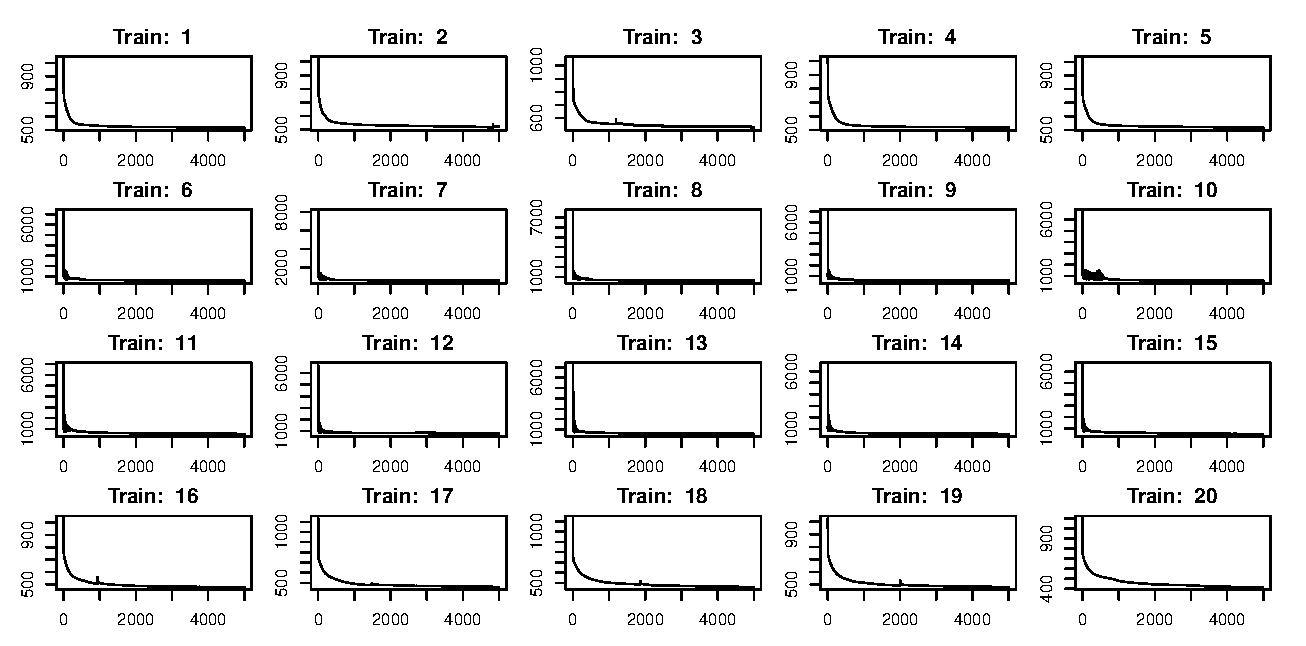
\includegraphics[width=5.5in]{04ANN/trainMammoSample.eps}
\end{center}
\caption{ตัวอย่างแสดง\textit{ค่าฟังชั่นเป้าหมาย}ระหว่างการฝึก ของการฝึกและประเมินผลครั้งที่ 1 ถึง 20 (จาก 45 ครั้ง).}
\label{fig: ann app train mamo 1-20}
\end{figure}
%

จากไฮเปอร์พารามิเตอร์ทั้ง 9 ชุดที่สนใจ และการทำครอสวาลิเดชั่นห้าพับสำหรับแต่ละชุด 
ทำให้มีการฝึกและประเมินผลทั้งหมดรวม $45$ ครั้ง.
ผู้สร้างโมเดลควรจะตรวจสอบการฝึกทั้ง $45$ ครั้งนี้.
รูป~\ref{fig: ann app train mamo 1-20} แสดงตัวอย่างของ\textit{ค่าฟังชั่นเป้าหมาย}ระหว่างการฝึก 
ของการฝึกและประเมินผลครั้งที่ 1 ถึง 20.
เส้นกราฟของค่าฟังชั่นเป้าหมายลดลงจนประมาณคงที่ในทุกๆรูปย่อย แสดงให้เห็นว่าการฝึกทั้งหมดเป็นไปด้วยดี.
สังเกตุว่า การฝึกครั้งที่ 10 ช่วงต้นมีการเปลี่ยนแปลงค่าฟังชั่นเป้าหมายต่อรอบฝึกค่อนข้างรุนแรง.
แต่ภายหลังจากราวๆ 1,000 รอบฝึก ค่าฟังชั่นเป้าหมายก็ลดลงด้วยดี จนเกือบคงที่ในรอบการฝึกท้ายๆ.

หลังจากได้ข้อสรุปสำหรับไฮเปอร์พารามิเตอร์แล้ว การสร้างโมเดลจะใช้ข้อมูลทั้งหมดทุกพับในการฝึกโมเดล 
และการประเมินประสิทธิภาพของโมเดลสุดท้ายที่ได้ ก็ทำด้วยข้อมูลที่แยกไว้ต่างหากอีกชุด (ไม่อยู่ในพับใดๆ).
ซึ่งสุดท้ายแล้ว ตัวอย่างนี้ได้โมเดลที่มี\textit{ค่าความแม่นยำ}เป็น $0.842$ (หรือ อัตราทายผิด $0.158$).
ตาราง~\ref{tbl: ann app precision recall} แจกแจงผลด้วย\textit{เมตริกซ์ความสับสน} (confusion matrix)
\index{confusion matrix}
ที่แสดง 
จำนวนที่ทายว่าเป็นกลุ่ม 1 และผลจริงก็เป็นกลุ่ม 1 (จำนวน\textit{บวกจริง}, true positive), 
จำนวนที่ทายว่าเป็นกลุ่ม 1 แต่ผลจริงเป็นกลุ่ม 0 (จำนวน\textit{บวกเท็จ}, false positive),
จำนวนที่ทายว่าเป็นกลุ่ม 0 แต่ผลจริงเป็นกลุ่ม 1 (จำนวน\textit{ลบเท็จ}, false negative), 
และ 
จำนวนที่ทายว่าเป็นกลุ่ม 0 และผลจริงก็เป็นกลุ่ม 0 (จำนวน\textit{ลบจริง}, true negative).
นอกจากนั้น ค่า\textit{ความเที่ยงตรง} (precision) และค่า\textit{การเรียกกลับ} (recall) ก็แสดงด้านข้างและด้านล่างของตารางตามลำดับ.

\begin{table}[hbtp]
%{\scriptsize
\caption{ผลประเมินของโครงข่ายที่ได้แสดงในรูปเมตริกซ์ความสับสน, ค่าความเที่ยงตรง, และค่าการเรียกกลับ}
\label{tbl: ann app precision recall}
\begin{center}
\begin{tabular}{ccccc}

        &       & \multicolumn{2}{c}{ผลจริง} & \\
        &       & 1              &   0      & \\
\cline{3-4}        
         &       & \multicolumn{1}{|c}{true positive} & \multicolumn{1}{|c|}{false positive} &  \\
ผลทำนาย   &     1 & \multicolumn{1}{|c}{162} & \multicolumn{1}{|c|}{17} & Precision = 0.905 \\
\cline{3-4}
         &      & \multicolumn{1}{|c}{false negative} & \multicolumn{1}{|c|}{true negative} & \\
         &     0 & \multicolumn{1}{|c}{56} & \multicolumn{1}{|c|}{227} & \\         
\cline{3-4}
         &       & Recall = 0.743 &               &
\end{tabular} 
\end{center}
%}%end \small
\end{table}

ถ้าจะอธิบายถึงค่า\textit{ความเที่ยงตรง}และค่า\textit{การเรียกกลับ}, 
ก็ควรอภิปรายถึง\textit{ความสมดุลของการกระจายของกลุ่มข้อมูล}ก่อน.
ข้อมูลชุดนี้มีการกระจายข้อมูลพอๆกัน ของข้อมูลกลุ่ม 1 (ผลเป็นเนื้อร้าย malignant) และข้อมูลกลุ่ม 0 (ผลเป็นเนื้อดี benign).
กล่าวคือ มีจำนวนระเบียนใกล้เคียงกัน นั่นคือ $445$ ระเบียน (กลุ่ม 1) และ $516$ ระเบียน (กลุ่ม 0).
ลักษณะการกระจายเช่นนี้ทำให้\textit{ค่าความแม่นยำ}สะท้อนกับคุณภาพการทำนายจริงของโมเดลได้ดี.
%
แต่หากการกระจายไม่สมดุลอย่างมาก เช่น สมมติอัตราส่วนคนเป็นมะเร็งตับอ่อนต่อประชากรมีค่าน้อยกว่า $1\%$ เพียงแต่โมเดลทำนายผลเป็นไม่เป็นมะเร็งสำหรับทุกๆตัวอย่างที่เข้ามาทดสอบ 
โมเดลนั้นก็มีโอกาสถูกถึง $99\%$ (ความแม่นยำ เป็น $0.99$)
นั่นคือ เท่ากับทายว่าไม่มีใครเป็นมะเร็งตับอ่อนเลย ซึ่งแม้จะมีโอกาสทายถูกสูงมากๆ 
แต่มันไม่ได้มีประโยชน์ต่อการช่วยระบุกลุ่มเสี่ยงเลย.

ดังนั้นแทนที่จะใช้แค่ค่าความแม่นยำ, ค่าความเที่ยงตรง (สมการ~\ref{eq: ann app precision 1}) และค่าการเรียกคืน (สมการ~\ref{eq: ann app recall 1}) 
จะช่วยสะท้อน\textit{คุณภาพการทำนายสำหรับข้อมูลที่มีการกระจายข้อมูลไม่สมดุล}ได้มากกว่า.

สำหรับงานจำแนกประเภทระหว่างสองกลุ่ม นั่นคือกลุ่มบวกและกลุ่มลบ.
ค่าความเที่ยงตรงสามารถคำนวณได้จาก
\begin{eqnarray}
   \mathrm{Precision} &=& \frac{\mathrm{True\; Positive}}{\mathrm{Predicted\; Positive}}
\label{eq: ann app precision 1} \\
   &=& \frac{\mathrm{True\; Positive}}{\mathrm{True\; Positive} + \mathrm{False\; Positive}}
\label{eq: ann app precision 2}
\end{eqnarray}
\index{precision}
เมื่อ $\mathrm{True\; Positive}$ คือจำนวนจุดข้อมูลที่ทำนายเป็นกลุ่มบวกและผลเฉลยเป็นกลุ่มบวก (บวกจริง)
และ $\mathrm{False\; Positive}$ คือจำนวนจุดข้อมูลที่ทำนายเป็นกลุ่มบวกแต่ผลเฉลยเป็นกลุ่มลบ
(บวกเท็จ)

ในทำนองเดียวกัน ค่าการเรียกกลับสามารถคำนวณได้จาก
\begin{eqnarray}
   \mathrm{Recall} &=& \frac{\mathrm{True\; Positive}}{\mathrm{Actual\; Positive}}
\label{eq: ann app recall 1} \\
   &=& \frac{\mathrm{True\; Positive}}{\mathrm{True\; Positive} + \mathrm{False\; Negative}}
\label{eq: ann app recall 2}
\end{eqnarray}
\index{recall}
เมื่อ $\mathrm{False\; Negative}$ คือจำนวนจุดข้อมูลที่ทำนายเป็นกลุ่มลบแต่ผลเฉลยเป็นกลุ่มบวก (ลบเท็จ)

หมายเหตุ เมื่อจะใช้ค่าความเที่ยงตรงและค่าการเรียกกลับในการวัดผล จะกำหนดให้ กลุ่ม 1 (กลุ่มบวก) เป็นกลุ่มที่มีสัดส่วนน้อย (เช่น กลุ่มของมะเร็งตับอ่อน) และกลุ่ม 0 (กลุ่มลบ) เป็นกลุ่มใหญ่ (เช่น กลุ่มที่ไม่ได้เป็น).

ค่าความเที่ยงตรงและค่าการเรียกกลับจะช่วยให้สะท้อนความสามารถของโมเดลได้ดีขึ้น โดยเฉพาะในกรณีที่ข้อมูลมีการกระจายระหว่างกลุ่มไม่สมดุล.
%
แต่การมีผลแสดงเป็นตัวเลข $2$ ค่านั้นอาจทำให้ลำบากในการเปรียบเทียบผล 
เช่น ผลของโมเดลหนึ่งอาจจะได้ค่าความเที่ยงตรงสูงแต่ค่าการเรียกกลับไม่มาก 
แต่อีกโมเดลหนึ่งที่มีค่าความเที่ยงตรงต่ำแต่ค่าการเรียกกลับสูงมาก.
ดังนั้น เพื่อความสะดวก ค่า\textit{คะแนนเอฟ} ($F$ Score หรือ บางครั้งเรียก $F_1$ Score) ซึ่งเป็นค่าเฉลี่ยเชิงเรขาคณิตจึงมักใช้ในการสรุป\textit{ค่าความเที่ยงตรง}และ\textit{ค่าการเรียกกลับ}เป็นตัวเลขตัวเดียว.
ค่า\textit{คะแนนเอฟ}สามารถคำนวณได้จาก,
\begin{eqnarray}
   F = 2 \cdot \frac{P \cdot R}{P + R}
\end{eqnarray}
เมื่อ $F$ แทนค่า\textit{คะแนนเอฟ}, $P$ และ $R$ แทนค่า\textit{ค่าความเที่ยงตรง}และ\textit{ค่าการเรียกกลับ}ตามลำดับ.
จากผลในตาราง~\ref{tbl: ann app precision recall} โมเดลในตัวอย่างจะมีค่า\textit{คะแนนเอฟ}เป็น $2 \cdot \frac{0.905 \cdot 0.743}{0.905 + 0.743} = 0.816$.

\section{ตัวอย่างการจำแนกประเภทแบบหลายกลุ่ม}
\label{section: multiclass example}

ห้วข้อนี้อภิปรายการจำแนกประเภทแบบหลายกลุ่ม โดยใช้ตัวอย่าง \textit{ข้อมูลชุดรูปของลายมือเขียนตัวเลข}.
\textit{ข้อมูลชุดรูปของลายมือเขียนตัวเลข} (Handwritten Digit Images) ได้มาจากการสแกนหน้าจดหมายของสำนักงานไปรษณีย์สหรัฐอเมริกา (U.S. Postal Service).
(ดู \cite{LeCunEtAl1990a} เพิ่มเติมสำหรับรายละเอียด)
ข้อมูลแต่ละภาพผ่านการจัดแนว (alignment), ซ่อมภาพเอียง (deslantation), และจัดขนาด (scaling). 
แต่ละระเบียน(จุดข้อมูล) มี $256$ มิติ (เก็บค่า $256$ ค่า) สำหรับค่าระดับสีเทาของ $256$ พิกเซลของแต่ละภาพลายมือเขียน ที่แต่ละภาพเป็นภาพของตัวเลขขนาด $16 \times 16$ พิกเซล.
ข้อมูลสามารถดาวน์โหลดได้จาก \url{http://statweb.stanford.edu/~tibs/ElemStatLearn/datasets/zip.info.txt}, \url{../zip.train.gz}, และ \url{../zip.test.gz} สำหรับคำอธิบาย, ข้อมูลชุดฝึกหัด และข้อมูลชุดทดสอบ ตามลำดับ.

{\small
\begin{shaded}
คำว่า``มิติ''มีความหมายเปลี่ยนแปลงตามบริบท.
\textit{มิติ}ของงานด้านภาพอาจทำให้ผู้อ่านสับสนกับ\textit{มิติ}ของจุดข้อมูล.
ภาพสองมิติจะจัดเรียงตามแนวนอนและแนวตั้ง เช่น ภาพขนาด $40 \times 30$ จะมีขนาด $40$ พิกเซลตามแนวนอน และ $30$ พิกเซลตามแนวตั้ง.
แต่เมื่อนำภาพหนึ่งภาพมาแปลงเป็นหนึ่งจุดข้อมูล ค่าของพิกเซลแต่ละค่าคือแต่ละมิติของจุดข้อมูล.
นั่นคือ ภาพสองมิติขนาด $40 \times 30$ หากแปลงเป็นจุดข้อมูล จะได้จุดข้อมูลที่มีขนาดมิติเป็น $1,200$ มิติ.
\end{shaded}
}%small

ตัวอย่างแสดงการใช้โครงข่ายประสาทเทียมสองชั้น 
โดยที่ชั้นเอาต์พุตใช้ฟังชั่นกระตุ้นเป็นฟังชั่นซอฟต์แมกซ์ (softmax function).
ประเด็นหนึ่งที่สำคัญคือการศึกษาความสัมพันธ์ระหว่างจำนวนหน่วยซ่อนกับผลการทำงาน.
%
รูป~\ref{fig: ann zip m 40 high rhos} แสดงความก้าวหน้าของการฝึกทั้ง $10$ ครั้ง
ของโครงข่ายประสาทเทียมขนาด $40$ หน่วยซ่อน. 
ทุกครั้ง โครงข่ายประสาทเทียมถูกฝึกด้วย\textit{วิธีลงเกรเดียนต์}และใช้\textit{ค่าอัตราการเรียนรู้}คงที่ตลอด.
นั่นคือ $\rho_h = 0.0002$ และ $\rho_o=0.002$, รอบฝึกสูงสุดคือ $500$ รอบ, 
ทำ\textit{การหยุดก่อนกำหนด} เมื่อค่าผิดพลาดของชุดข้อมูลวาลิเดชั่นเพิ่มขึ้นจากค่าที่ดีที่สุดมากกว่า $1$ เท่าตัว.
ค่าเริ่มต้นของ\textit{ค่าน้ำหนัก}ทุกค่าสุ่มมาจากช่วง $[-0.1,0.1]$ ตามการแจกแจงเอกรูป (uniform distribution).

การที่ทำการฝึก $10$ ครั้ง ก็เพื่อหาครั้งที่ดีที่สุด จากการสุ่มค่าน้ำหนักเริ่มต้น.
สังเกตุ มีการฝึกหลายครั้งที่ยังไม่ถึงการลู่เข้า เช่น การฝึกที่ 3, 8 และ 9.
การฝึกเหล่านี้แม้เพิ่มจำนวนรอบฝึกก็จะไม่ช่วยอะไร 
เพราะ การฝึกทั้ง $10$ ครั้งนี้ ทุกครั้งหยุดก่อน $500$ รอบฝึก ซึ่งเป็นจำนวนรอบฝึกสูงสุดที่ตั้งไว้.
ที่เป็นเช่นนี้ได้ ก็เพราะมีทำ\textit{การหยุดก่อนกำหนด} (Early Stopping ดูหัวข้อ~\ref{sec: ann early stopping}).
ข้อสัณณิฐานเบื้องต้นคือ ค่า\textit{อัตราการเรียนรู้}ที่ใช้อาจใช้ค่าสูงเกินไป 
ทำให้เมื่อการฝึกเข้าใกล้ค่าที่ดีที่สุด แล้วค่าน้ำหนักถูกปรับให้เลย\textit{จุดดีที่สุด} 
และอาจทำให้ผลวาลิเดชั่นแย่ลง ซึ่งส่งผลให้เกิดการหยุดก่อนกำหนดขึ้น.
การไม่ทำการหยุดก่อนกำหนด ก็อาจเป็นวิธีหนึ่ง แต่อาจนำปัญหาอื่นมาให้ 
เช่น อาจทำให้เสียเวลาฝึกนานขึ้น แต่กลับได้โมเดลที่โอเวอร์ฟิตกับข้อมูลฝึกหัด แต่ไม่สามารถทำนายได้ดีกับข้อมูลที่ต้องการใช้งานจริง (เสียคุณสมบัติความทั่วไป).
สิ่งที่ควรทำสำหรับกรณีนี้ คือ ทดลองลดค่าอัตราการเรียนรู้ลง ได้แก่ ลองใช้ $\rho_h=0.0001$ และ $\rho_o=0.001$.
ผลการฝึกด้วยค่าอัตราการเรียนรู้ที่น้อยลงแสดงดังรูป~\ref{fig: ann zip m 40 good rhos}.

%
\begin{figure}
\begin{center}
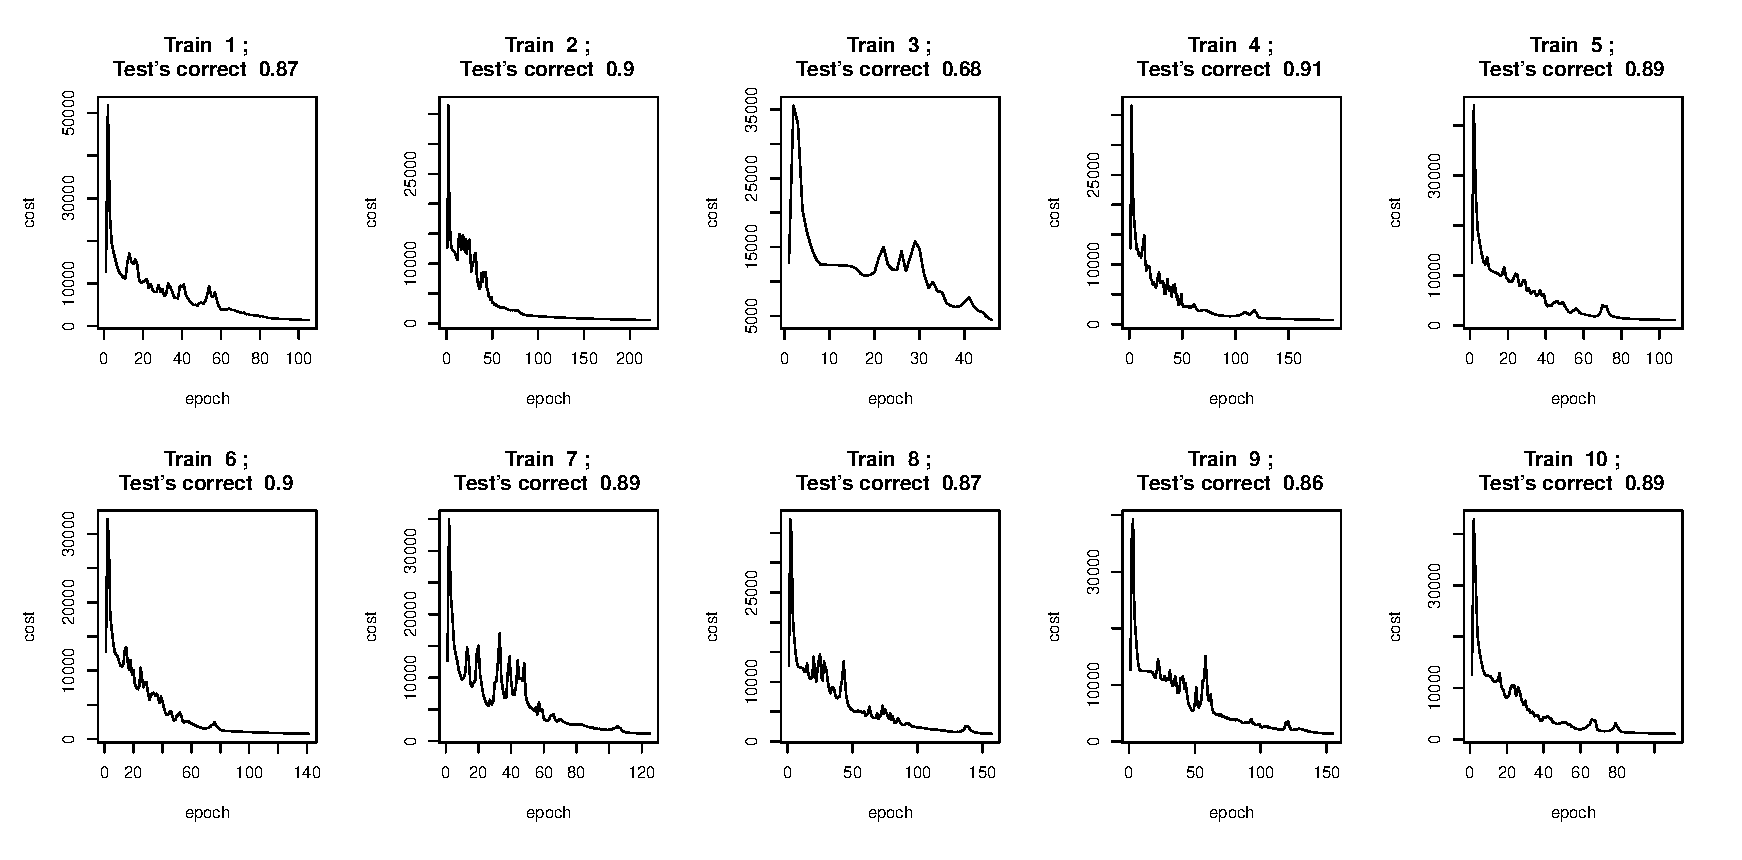
\includegraphics[width=5.5in]{04ANNAppImg/m40trainCost.eps}
\end{center}
\caption{ผลการฝึกโครงข่ายประสาทเทียมขนาดสี่สิบหน่วยซ่อน $10$ ครั้ง. 
สังเกตุการที่การฝึกหยุดก่อนจำนวนรอบการฝึกที่กำหนด (ซึ่งคือ $500$ รอบฝึก) ก็เพราะการทำหยุดก่อนกำหนด 
และ อาจเป็นเพราะการเลือกใช้ค่าอัตราการเรียนรู้ที่สูงเกินไป.}
\label{fig: ann zip m 40 high rhos}
\end{figure}
%

รูป~\ref{fig: ann zip m 40 good rhos} แสดงการลู่เข้าในทุกๆการฝึก และทุกการฝึกสามารถทำจนครบรอบฝึกสูงสุด.
ข้อสัณณิฐานเบื้องต้นน่าจะถูกต้อง.
นั่นคือ ค่าอัตราการเรียนรู้ของการฝึกครั้งแรกมากเกินไป (รูป~\ref{fig: ann zip m 40 high rhos}).
สังเกตุว่า นอกจากทุกๆการฝึกถึงการลู่เข้า แล้วผลการทดสอบยังดีขึ้นด้วย.
นั่นคือ ค่าความแม่นยำ (\texttt{Test's correct} ในรูป) ซึ่งคือ อัตราการทายถูกเมื่อทดสอบกับข้อมูลชุดทดสอบ มีค่าเพิ่มจากช่วงค่า $0.68$ ถึง $0.91$ ในครั้งแรก (รูป~\ref{fig: ann zip m 40 high rhos}) เป็น $0.92$ ถึง $0.93$ (รูป~\ref{fig: ann zip m 40 good rhos}).

%
\begin{figure}
\begin{center}
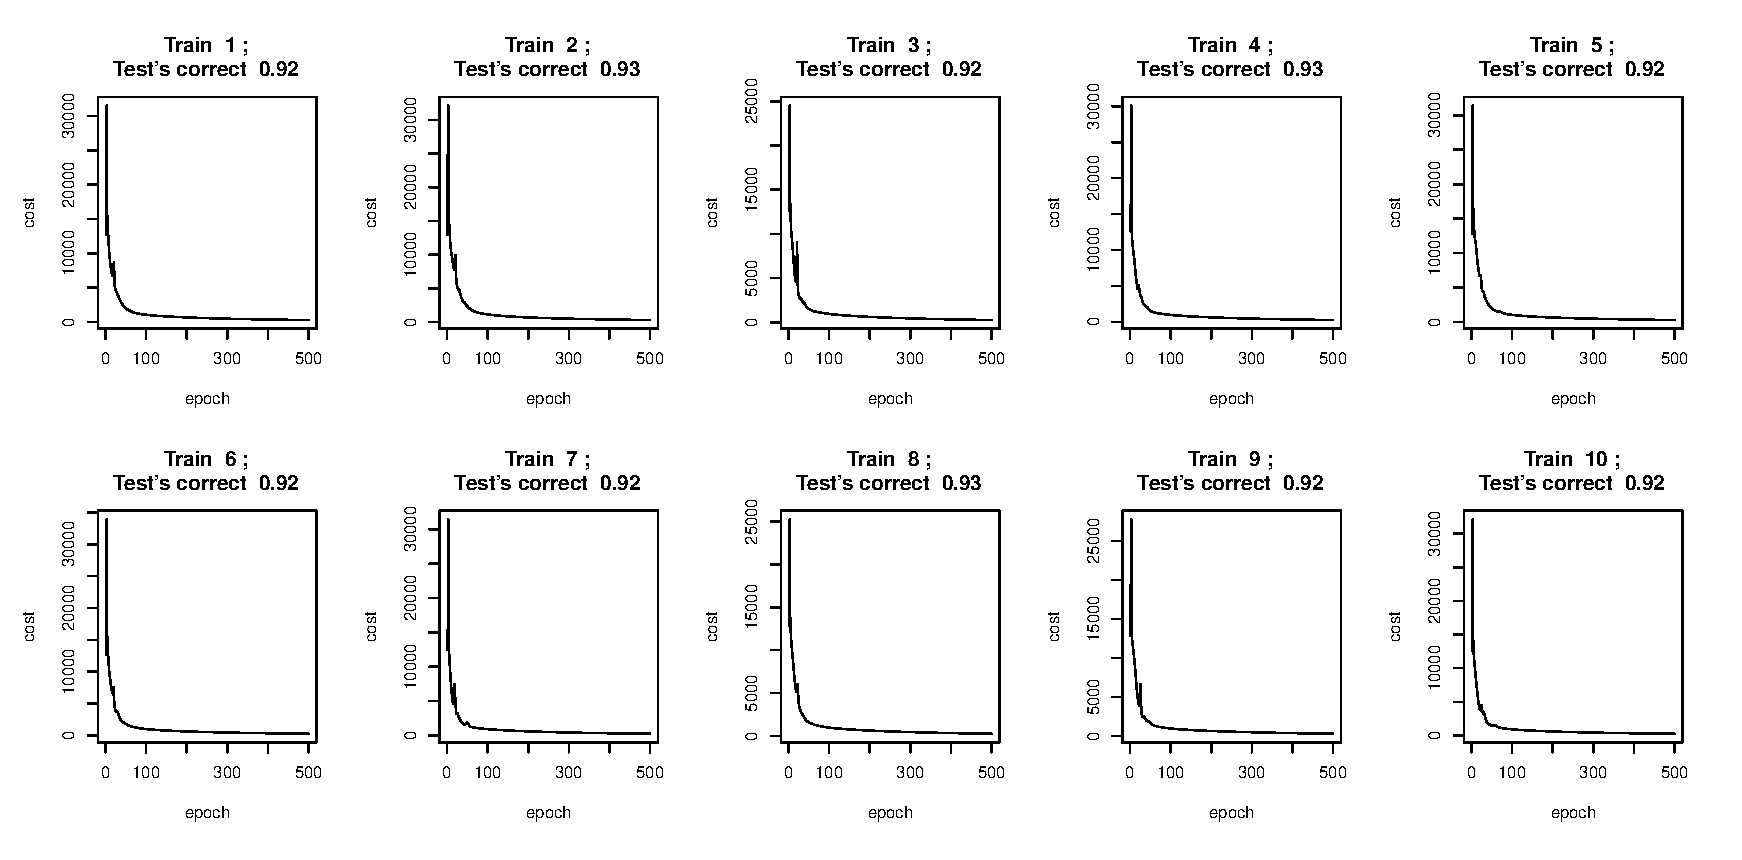
\includegraphics[width=5.5in]{04ANNAppImg/m40trainCostLowRho.eps}
\end{center}
\caption{ผลการฝึกโครงข่ายประสาทเทียมขนาดสี่สิบหน่วยซ่อน $10$ ครั้ง ที่ใช้ค่าอัตราการเรียนรู้น้อยลง จากการฝึกที่แสดงในรูป~\ref{fig: ann zip m 40 high rhos}.}
\label{fig: ann zip m 40 good rhos}
\end{figure}
%

ในลักษณะเดียวกัน การทดลองฝึกโครงข่ายประสาทเทียมที่มีจำนวนหน่วยซ่อนต่างๆให้ผลดังแสดงในรูป~\ref{fig: ann zip multiple Ms}.
เช่นเดียวกับแนวปฏิบัติที่ดีในการฝึกโครงข่ายประสาทเทียมทั่วๆไป ต้องมีการตรวจสอบดูว่าการฝึกเป็นไปอย่างสมบูรณ์ 
เพราะการจะสรุปผลได้อย่างถูกต้องว่าจำนวนหน่วยซ่อนเท่าใดดีกว่า 
ต้องอยู่บนพื้นฐานว่าการฝึกทำได้อย่างสมบูรณ์สำหรับจำนวนหน่วยซ่อนนั้นๆแล้ว.

สังเกตุว่า หากจำนวนหน่วยซ่อนน้อยเกินไป การเพิ่มจำนวนหน่วยซ่อนสามารถช่วยเพิ่มความถูกต้องในการจำแนกได้ แต่พอจำนวนหน่วยซ่อนเพียงพอแล้ว ($20$ หน่วยซ่อน) การเพิ่มจำนวนหน่วยซ่อน (เป็น $40$ หน่วยซ่อน) ไม่ได้ช่วย เพิ่มความแม่นยำขึ้นเลย.
การใช้หน่วยซ่อนมากเกินความจำเป็นไม่สามารถเพิ่มความแม่นยำขึ้นได้ แต่การคำนวณจะต้องทำมากขึ้น ตามจำนวนค่าน้ำหนักที่มากขึ้น.
นั่นคือ $\mathbf{W}^{(1)}$ และ $\mathbf{W}^{(2)}$ เป็นเมตริกซ์ขนาด $[M \times (D+1)]$ และ $[K \times (M+1)]$ 
ดังนั้น ที่ $20$ หน่วยซ่อน, ค่าน้ำหนัก เป็นเมตริกซ์ขนาด $[20 \times 257]$ และ $[10 \times 21]$ ตามลำดับ และ ที่ $40$ หน่วยซ่อน, ค่าน้ำหนัก เป็นเมตริกซ์ขนาด $[40 \times 257]$ และ $[10 \times 41]$ ตามลำดับ.
ดังนั้นตัวอย่างนี้จึงเลือกใช้โครงข่ายประสาทเทียมที่มีจำนวน $20$ หน่วยซ่อน 
และเมื่อนำผลทดสอบมาแสดงในเมตริกซ์แจงความสับสน (confusion matrix) จะได้ตาราง~\ref{tbl: ann app zip image confusion matrix}.

%
\begin{figure}
\begin{center}
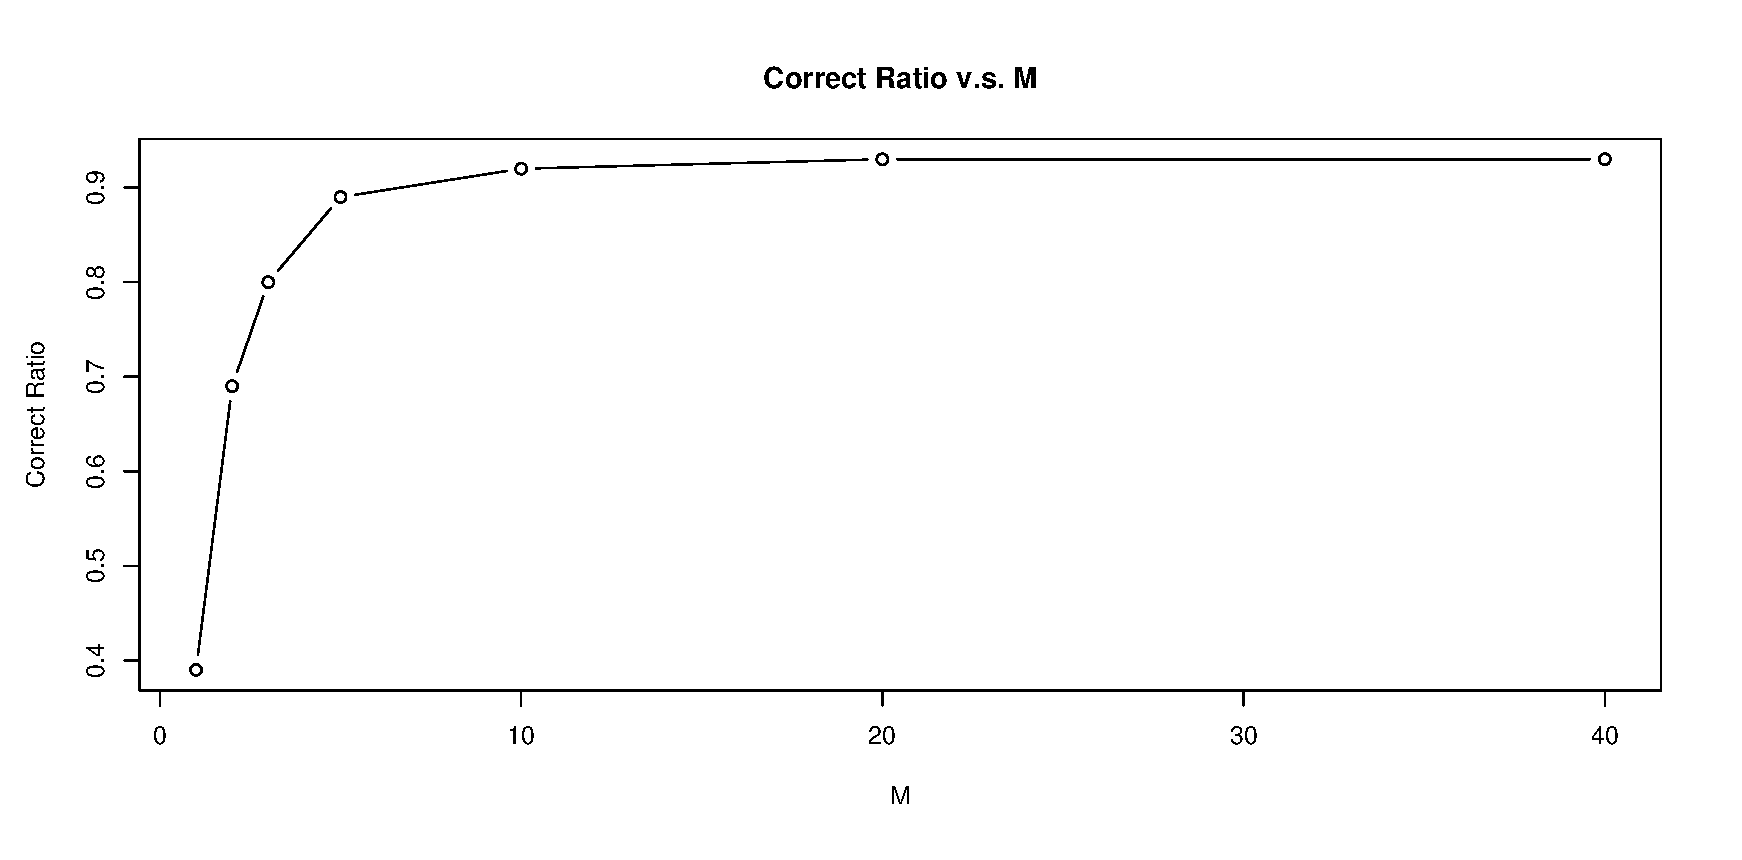
\includegraphics[width=5.5in]{04ANNAppImg/zipComporingMs.eps}
\end{center}
\caption{ผลการฝึกโครงข่ายประสาทเทียมขนาดหน่วยซ่อนต่างๆ.}
\label{fig: ann zip multiple Ms}
\end{figure}
%

\begin{table}[hbtp]
%{\scriptsize
\caption{ผลประเมินของโครงข่ายที่ได้ในรูปเมตริกซ์แจงความสับสน}
\label{tbl: ann app zip image confusion matrix}
\begin{center}
\begin{tabular}{|c|c|c|c|c|c|c|c|c|c|c|}
\hline
& \multicolumn{10}{|c|}{กลุ่มจริง} \\
\cline{2-11}
ผลทายกลุ่ม & 0 & 1 & 2 & 3 & 4 & 5 & 6 & 7 & 8 & 9 \\
\hline
0 & 348  & 0  & 3  & 2  & 2  & 3  & 0  & 0  & 5  & 0  \\
\hline
1 & 0  & 254  & 0  & 0  & 2  & 0  & 0  & 0  & 0  & 2  \\
\hline
2 & 2  & 0  & 178  & 3  & 3  & 0  & 2  & 1  & 2  & 1  \\
\hline
3 & 2  & 0  & 3  & 146  & 0  & 7  & 0  & 1  & 4  & 0  \\
\hline
4 & 2  & 2  & 4  & 1  & 180  & 3  & 3  & 7  & 0  & 3  \\
\hline
5 & 1  & 0  & 1  & 9  & 3  & 143  & 4  & 0  & 4  & 0  \\
\hline
6 & 2  & 2  & 1  & 0  & 2  & 0  & 161  & 0  & 1  & 0  \\
\hline
7 & 0  & 2  & 2  & 2  & 1  & 1  & 0  & 134  & 0  & 3  \\
\hline
8 & 1  & 1  & 6  & 2  & 2  & 1  & 0  & 1  & 149  & 2  \\
\hline
9 & 1  & 3  & 0  & 1  & 5  & 2  & 0  & 3  & 1  & 166  \\
\hline
\end{tabular} 
\end{center}
%}%end \small
\end{table}

ข้อมูลชุดทดสอบมีขนาด $2007$ ระเบียน 
และโครงข่ายทายผิดทั้งหมด $148$ ระเบียน คิดเป็น $7.37\%$.
ตัวอย่างของระเบียนที่ทายผิดแสดงในรูป~\ref{fig: ann zip wrong classified samples}.

%
\begin{figure}
\begin{center}
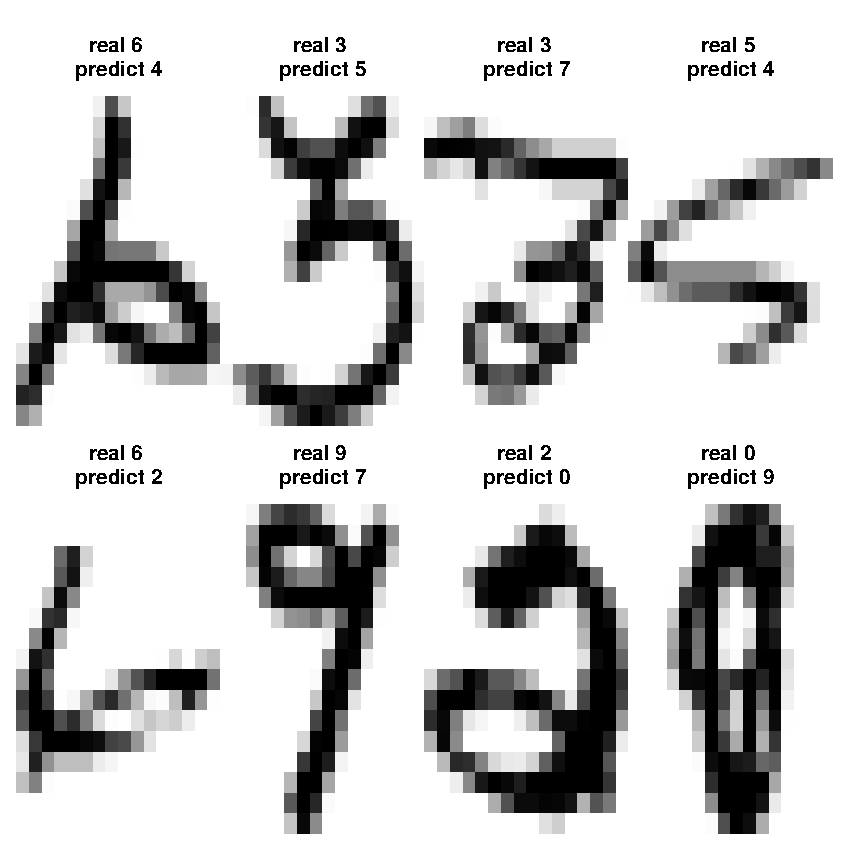
\includegraphics[width=4in]{04ANNAppImg/sampleWrongClass.eps}
\end{center}
\caption{ตัวอย่างของรูปที่ทายผิด. กลุ่มที่ถูกต้อง (real) และ ผลการทาย (predict) เขียนกำกับไว้เหนือแต่ละรูป.}
\label{fig: ann zip wrong classified samples}
\end{figure}
%

%{\small
%\begin{shaded}
%[Free will v.s. Free won't]
%\textit{เจตจำนงค์อิสระ} (free will)
%\textit{การสะกดจิต} (hypnosis)
%\end{shaded}
%}%small

\section{อาร์โค้ด}
\label{sec: ann R codes}

\textit{อาร์โค้ด}ในหัวข้อนี้ดัดแปลงมาจาก\textit{อาร์โค้ด}ของสื่อประกอบการสอนของแอนเดอร์ซัน\footnote{Charles Anderson, สื่อประกอบการเรียน วิชา CS545 Machine Learning, Fall 2006, Department of Computer Science, Colorado State University, Fort Collins, CO, USA.}

\subsection{โค้ดสำหรับตัวอย่างง่ายๆ}
\label{sec: ann app code simple example}

รายการ~\ref{lst: ann nnOutput} แสดง\textit{อาร์โค้ด}สำหรับ\textit{ซิกมอยด์ฟังชั่น} (\texttt{sigmoid}), อนุพันธ์ของซิกมอยด์ฟังชั่น (\texttt{dsigmoid}), และฟังชั่นคำนวณค่าของโครงข่าย (\texttt{nnOutput}).
โดยฟังชั่น \texttt{nnOutput} รับค่าพารามิเตอร์ของโครงข่าย (ตัวแปร \texttt{net}), 
อินพุต (ตัวแปร \texttt{X}), 
และชนิดปัญหาที่โครงข่ายทำงาน (ตัวแปร \texttt{nntype}).
ตัวแปร \texttt{net} เป็นตัวแปรชนิด \texttt{list} ที่ต้องประกอบด้วย \texttt{net\$W1} และ \texttt{net\$W2} ที่เป็นเมตริกซ์ ขนาด $M \times (D+1)$ และ $K \times (M+1)$ สำหรับค่าน้ำหนักชั้นที่ 1 และ 2 ตามลำดับ,
เมื่อ $D$ คือ จำนวนมิติของอินพุต \texttt{X};
 $M$ คือ จำนวนหน่วยซ่อน;
 และ $K$ คือ จำนวนมิติของเอาต์พุตโครงข่าย.
ฟังชั่น \texttt{nnOutput} ทำการคำนวณสมการ~\ref{eq: ANN 2-layer x dot}, \ref{eq: ANN 2-layer z}, \ref{eq: ANN 2-layer z dot}, และ \ref{eq: ANN 2-layer output matrix}.
ตาราง~\ref{tbl: ANN output activation function} สรุป\textit{ฟังชั่นกระตุ้น}ของชั้นเอาต์พุตที่ขึ้นกับชนิดปัญหา.
อาร์กูเมนต์ \texttt{nntype} ใช้ระบุชนิดปัญหา และมีค่าดีฟอล์ตเป็นชนิดปัญหาการหาค่าถดถอย.

\lstinputlisting[language=R, caption={ซิกมอยด์ฟังชั่น (\texttt{sigmoid}), อนุพันธ์ของซิกมอยด์ฟังชั่น (\texttt{dsigmoid}), และฟังชั่นคำนวณค่าของโครงข่าย (\texttt{nnOutput})}, 
label={lst: ann nnOutput}]{04ANN/nnOutputCode.r}

สังเกตุ $h'(a) = h(a) \cdot (1 - h(a))$ 
แต่ \texttt{dsigmoid} ใช้ \texttt{(1 - z)*z} 
เพราะว่า \texttt{dsigmoid} รับอาร์กูเมนต์เป็น ตัวแปร \texttt{z} ซึ่งคือ $h(a)$.
การทำเช่นนี้จะช่วยลดการคำนวณซ้ำซ้อนลงไปได้.

รายการ~\ref{lst: ann nntrain} แสดงโค้ดของฟังชั่นฝึกโครงข่าย \texttt{nnTrain} สำหรับโครงข่ายสองชั้น.
ฟังชั่น \texttt{nnTrain} รับอาร์กูเมนต์เป็น อินพุตของข้อมูลชุดฝึก \texttt{X}, เอาต์พุตของข้อมูลชุดฝึก \texttt{T}, จำนวนหน่วยซ่อน \texttt{nHidden}, อัตราเรียนรู้สำหรับน้ำหนักชั้นซ่อนและชั้นเอาต์พุต \texttt{rhoh} และ \texttt{rhoo} ตามลำดับ.
นอกจากอาร์กูเมนต์ข้างต้น \texttt{nnTrain} ยังอนุญาติให้เลือกช่วงค่าของน้ำหนักตอนเริ่มต้นผ่านตัวแปร \texttt{wmax}, เลือกจำนวนรอบฝึกผ่านตัวแปร \texttt{nEpoch}, เลือกที่จะทำการวาดกราฟแสดงค่าผิดพลาดขณะฝึกหรือไม่ผ่านตัวแปร \texttt{graph}, และให้เลือกที่จะใส่โครงข่าย \texttt{net} เข้ามาเพื่อฝึกต่อได้.
เพื่อให้แน่ใจว่าโค้ดของ\textit{การแพร่กระจายย้อนกลับ}ทำได้อย่างถูกต้อง, 
ควรเปรียบเทียบผลกับการคำนวณค่าเกรเดียนต์แบบเชิงเลขด้วย (ดูแบบฝึกหัดข้อ 11)

\lstinputlisting[language=R, caption={ฟังชั่นฝึกโครงข่าย (\texttt{nnTrain})},
label={lst: ann nntrain}]{04ANN/nnTrainCode.r}

สังเกตุภายในโค้ดว่า ถ้าไม่มีการใส่ \texttt{net} เป็นอาร์กูเมนต์ (เท่ากับ \texttt{net} เป็น \texttt{NULL}),
โปรแกรมก็จะเริ่มสุ่มกำหนดค่าเริ่มต้นให้กับน้ำหนักชั้นที่ 1 และ 2 คือ \texttt{W1} และ \texttt{W2} ตามลำดับ.
ตัวแปร \texttt{errors} มีไว้เพื่อเก็บประวัติ\textit{ค่าผิดพลาด}ระหว่างการฝึก.
\\
\underline{หมายเหตุ} 
โค้ดในรายการ~\ref{lst: ann nntrain} ใช้ค่าที่เก็บใน \texttt{errors} 
เป็น \verb|sqrt(mean(DELTA2^2))|, 
ซึ่งคือ ค่า $\sqrt{\frac{1}{N} \sum_{n=1}^N \Vert \mathbf{y}(\mathbf{x}_n, \mathbf{w}) - \mathbf{t}_n \Vert^2}$, เรียกว่า ค่าอาร์เอมเอส (rms).
ค่านี้ไม่ใช่ค่าฟังชั่นจุดประสงค์ ซึ่งคือ $\frac{1}{2} \sum_{n=1}^N \Vert \mathbf{y}(\mathbf{x}_n, \mathbf{w}) - \mathbf{t}_n \Vert^2$ (สมการ~\ref{eq: ANN error function}).
แต่ค่าอาร์เอมเอสนี้จะเป็นสัดส่วนตามฟังชั่นจุดประสงค์ จึงสามารถใช้ตรวจสอบความก้าวหน้าของการฝึกได้.

นอกจากนั้น โค้ดในรายการ~\ref{lst: ann nntrain} ทำ\textit{การคำนวณไปข้างหน้า} (forward pass) ด้วยฟังชั่นกระตุ้นสำหรับปัญหาการหาค่าถดถอย.
สำหรับปัญหาชนิดอื่น \textit{ฟังชั่นกระตุ้นชั้นเอาต์พุต}จะต้องถูกเปลี่ยนให้เหมาะสม ตามที่อภิปรายในหัวข้อ~\ref{sec: ANN Activation Function}.

เมื่อทำการเปรียบเทียบสมการ~\ref{eq: ANN BP delta k},~\ref{eq: ANN BP delta j} และ~\ref{eq: ANN BP dE/dw} กับโค้ด \texttt{nnTrain} จะเห็นว่า ฟังชั่น \texttt{nnTrain} ทำการคำนวณการแพร่กระจายย้อนกลับ และใช้วิธีลงเกรเดียนต์ในการฝึกโครงข่าย.
สุดท้าย \texttt{nnTrain} ส่งผลลัพธ์ที่ได้ออกมาผ่านตัวแปรชนิด \texttt{list} (ที่มีส่วนสำคัญที่สุดคือ ค่าน้ำหนัก \texttt{W1} กับ \texttt{W2}).

ฟังชั่นที่สำคัญอีกอย่างคือส่วนที่ใช้ทำนอร์มอไลเซชั่น (ฟังชั่น \texttt{normalize}) ซึ่งแสดงในรายการ~\ref{lst: ann normalize}.
ฟังชั่นที่แสดงนี้ทำนอร์มอไลเซชั่นแบบปรับค่าค่าเฉลี่ยและค่าเบี่ยงเบนมาตราฐาน (หัวข้อ~\ref{section: normalization}).

สังเกตุ \texttt{stdevs[stdevs==0] <- 1} ทำเพื่อป้องกันปัญหาเชิงคำนวณ ที่เมื่ออินพุตบางมิติมีค่าเดียวตลอด (ทำให้ค่าเบี่ยงเบนมาตราฐานเป็น $0$ และจะทำให้เกิดการหารด้วย $0$ เกิดขึ้น).
วิธีนี้เป็นทางแก้ชั่วคราว.
วิธีที่ดีกว่าคือ ถ้าเกิดสถานะการณ์ที่มีค่าอินพุตบางมิติมีค่าเดียวตลอด, 
การฝึกโครงข่ายอาจจะพิจารณาตัดมิตินั้นออกไปเลย 
เพราะการที่อินพุตมิตินั้นไม่เคยเปลี่ยนแปลงเลย 
อินพุตมิตินั้นจะไม่มีผลช่วยให้ทำนายเอาต์พุตได้ดีขึ้นเลย 
แต่การมีมิติมากขึ้นทำให้โครงข่ายต้องทำการคำนวณมากขึ้น.

สังเกตุเพิ่มเติมอีกว่า ฟังชั่น \texttt{normalize} อนุญาติให้เลือกได้ว่าจะให้ฟังชั่นทำการคำนวณค่าเฉลี่ย (\texttt{means}) กับ ค่าเบี่ยงเบนมาตราฐาน (\texttt{stdevs}) เอง 
หรือ อนุญาติให้ผู้ใช้สามารถระบุค่าเฉลี่ยกับค่าเบี่ยงเบนมาตราฐานเข้าเป็นอาร์กูเมนต์ก็ได้.
รวมทั้ง ผู้ใช้สามารถเลือกให้ฟังชั่น นอกจากทำนอร์มอไลเซชั่นของค่าที่ต้องการแล้ว ยังให้มันบอกค่า \texttt{means} และ \texttt{stdevs} ที่ใช้ทำนอร์มอไลเซชั่นออกมาได้ด้วย.
ผู้ใช้ต้องการค่า \texttt{means} และ \texttt{stdevs} ที่ใช้ในการทำนอร์มอไลเซชั่นนี้
เพราะ หากมีการทำนอร์มอไลเซชั่นกับอินพุตของข้อมูลฝึกหัด ด้วย \texttt{means} และ \texttt{stdevs} ค่าเท่าใด 
ผู้ใช้ก็ควรจะใช้ค่าเท่านั้นในการทำนอร์มอไลเซชั่นกับอินพุตของข้อมูลทดสอบหรือข้อมูลที่จะใช้งานด้วย.

\lstinputlisting[language=R, caption={ฟังชั่นทำนอร์มอไลเซชั่น (\texttt{normalize})},
label={lst: ann normalize}]{04ANN/normalizeCode.r}

ตัวอย่างง่ายๆ (หัวข้อ~\ref{sec: simple example}) เตรียมข้อมูลจากโค้ดที่แสดงในรายการ~\ref{lst: ANN simple create data}.
สังเกตุว่าเมื่อทำนอร์มอไลเซชั่น ทำนอร์มอไลเซชั่นของอินพุตทั้งชุดฝึกและชุดทดสอบ 
และการทำนอร์มอไลเซชั่นของชุดทดสอบก็ใช้พารามิเตอร์ของนอร์มอไลเซชั่นค่าเดียวกับชุดฝึก (ดูตัวแปร \texttt{r\$means} และ \texttt{r\$stdevs}).

\begin{lstlisting}[language=R,caption={เตรียมข้อมูลสำหรับตัวอย่างง่ายๆ},
label={lst: ANN simple create data}]
f <- function (x) { x + 8 * sin(x) + rnorm(length(x)) }

N <- 50
train.X <- matrix(seq(0,4*pi,len=N),1,N)
train.T <- f(train.X)
r <- normalize(train.X,returnParms=TRUE)
train.Xn <- r$data
  
test.X <- matrix(seq(0,4*pi,len=round(N/3)),nrow=1)
test.T <- f(test.X)
test.Xn <- normalize(test.X,r$means,r$stdevs)
\end{lstlisting}

ฟังชั่น \texttt{nnTrain} สร้างและฝึกโครงข่ายประสาทเทียม เช่น
\begin{verbatim}
      net <- nnTrain(train.Xn,train.T, nHiddens=20, 
                   rhoh=0.01,rhoo=0.0003, wmax=0.5, nEpochs=9001)
\end{verbatim}
ซึ่งจะสร้างโครงข่ายประสาทเทียมสองชั้นขนาด $20$ หน่วยซ่อน 
และกำหนดค่าเริ่มต้นของค่าน้ำหนักโดยสุ่มจากช่วง $[-0.5, 0.5]$ 
ทำการฝึก $9001$ รอบกับข้อมูลที่มีอินพุตเป็น \texttt{train.Xn} และเอาต์พุตเป็น \texttt{train.T} 
ฝึกด้วย\textit{ค่าอัตราการเรียนรู้} $\rho_h = 0.01$ และ $\rho_o = 0.0003$ 
สำหรับ\textit{ชั้นซ่อน}และ\textit{ชั้นเอาต์พุต}ตามลำดับ.
%หมายเหตุ โค้ดที่แสดง เป็นโค้ดที่เทียบเท่ากับ โค้ดที่ใช้เตรียมตัวอย่างหัวข้อ~\ref{sec: simple example} ที่มีความซับซ้อนกว่าเล็กน้อย.

เมื่อฝึกโครงข่ายประสาทเทียมเสร็จ โครงข่ายที่ฝึกแล้วถูกทดสอบโดยการนำไปทำนายผลอินพุตของ\textit{ข้อมูลชุดทดสอบ} ดังนี้
\begin{verbatim}
   test.y <- nnOutput(net,test.Xn)
\end{verbatim}
และค่าที่ทำนายของชุดทดสอบถูกนำไปเปรียบเทียบกับเอาต์พุตจริง (เฉลยของข้อมูลชุดทดสอบ),
\begin{verbatim}
   test.rmse <- sqrt(mean((test.y - test.T)^2))
\end{verbatim}
ซึ่งตัวอย่างนี้ได้\textit{ค่าผิดพลาด}เป็น $1.54$ ดังแสดงในรูป~\ref{fig: ANN simple example results}.
โค้ดข้างต้นไม่จำเป็นต้องระบุ \texttt{nntype='regression'} 
เพราะ\textit{การหาค่าถดถอย}เป็น\textit{ค่าดีฟอล์ต}สำหรับฟังชั่น \texttt{nnOutput} อยู่แล้ว.

\paragraph{สำหรับการทำการหยุดก่อนกำหนด}
การเพิ่มการทำ\textit{การหยุดก่อนกำหนด}ก็เพียงแค่ดัดแปลงโค้ดในรายการ~\ref{lst: ann nntrain} 
โดยเพิ่มอาร์กูเมนต์เข้าไปตอนนิยามฟังชั่น เช่น
\begin{verbatim}
nnTrain <- function (X,T,nHiddens,rhoh,rhoo,wmax=0.1,nEpochs,
   graph=TRUE,net=NULL, earlystopping=FALSE, early.tol=0.1,  
   val.X=NULL, val.T=NULL)
\end{verbatim}
โดย $2$ บรรทัดท้ายเพิ่มทางเลือก \texttt{earlystopping} เพื่อเป็นตัวแปรกำหนดว่าจะทำหยุดก่อนกำหนดหรือไม่ (\textit{ค่าดีฟอล์ต}คือไม่ทำ).
นอกจากอินเตอร์เฟซของฟังชั่น ภายในตัวฟังชั่น (function body, ก่อนบรรทัดที่ 61 ของรายการ~\ref{lst: ann nntrain}) ก็เพิ่มโค้ด ดังนี้
\begin{verbatim}
if (earlystopping) {
  val.Y <- nnOutput(list(W1=W1, W2=W2), val.X)
  val.E <- sum( (val.Y - val.T)^2 )

  if (val.E < best.val.E) {
    best.net <- list(W1=W1, W2=W2, Z=Z, Y=Y, errors=errors)
    best.val.E <- val.E

  } else if( val.E > (1 + early.tol) * best.val.E ) break;

}##end if
\end{verbatim}

สังเกตุว่า โค้ดข้างต้นยอมให้ค่าผิดพลาดของชุดวาลิเดชั่นเพิ่มขึ้นได้บ้าง
ตัวอย่างเช่น \texttt{early.tol=0.1} คือ ยอมให้เพิ่มขึ้นได้ไม่เกิน $10\%$.
หรือ หากต้องการ อาจใช้จำนวนครั้งที่ยอมให้ค่าผิดพลาดของชุดวาลิเดชั่นเพิ่มขึ้น เป็นเงื่อนไขของการหยุดการฝึกก็ได้ 
หรือ แม้แต่อาจใช้เงื่อนไขหลายๆอย่างผสมกันได้ ดังเช่น การทำงานของ\textit{ชุดเครื่องมือโครงข่ายประสาทเทียมของโปรแกรมแมทแลป} (Matlab's neural network toolbox) ซึ่งเป็นชุดซอฟต์แวร์สำหรับโครงข่ายประสาทเทียมของบริษัทแมธเวิร์ค (MathWorks) ที่มีการใช้เงื่อนไขผสม 
เพื่ออนุญาติให้ผู้ใช้เลือก\textit{การหยุดก่อนกำหนด}ให้เหมาะสมกับปัญหาที่ทำได้.

\subsection{โค้ดสำหรับตัวอย่างการหาค่าถดถอย (ข้อมูลชุดเรือยอชต์)}
\label{sec: regression example code}

ข้อมูล \texttt{yacht\_hydrodynamics.data} อยู่ในรูปแบบแฟ้มข้อความ (textfile) 
ที่แต่ละระเบียนแสดงเป็นบรรทัด.
ข้อมูลนี้สามารถถูกนำเข้าได้ดังนี้
\begin{verbatim}
   y.dat <- read.csv("yacht_hydrodynamics.data", sep = " ")
\end{verbatim}
ซึ่งอาร์กูเมนต์ \texttt{sep = " "} ระบุว่าแต่ละเขตข้อมูลใน \texttt{yacht\_hydrodynamics.data} จะคั่นด้วยช่องว่าง (สังเกตุเนื้อหาในไฟล์ \texttt{yacht\_hydrodynamics.data}%
\footnote{%
บางครั้งอาจต้องทำการจัดการไฟล์ข้อมูลก่อนที่จะสามารถนำข้อมูลเข้ามาได้อย่างถูกต้อง
เช่น ไฟล์ข้อมูล \texttt{yacht\_hydrodynamics.data} ที่ใช้ช่องว่างสองช่องติดกัน แทนที่จะใช้แค่ช่องเดียว.
เพื่อให้ฟังชั่น \texttt{read.csv} โหลดข้อมูลได้ถูกต้อง (ผลลัพธ์มีขนาด $307 \times 7$)
อาจทำการจัดการแก้ไขให้ช่องว่างสองช่องที่ติดกัน โดยแก้ให้เป็นช่องเดียวก่อน ด้วยฟังชั่น \texttt{Replace} ซึ่งมีใน\textit{โปรแกรมจัดการไฟล์ข้อความ}ทั่วไป.
}).

เมื่อนำเข้าข้อมูลเรียบร้อย ข้อมูลส่วนหนึ่งควรจะถูกกันไว้เพื่อการตรวจสอบประสิทธิผลของการทำนาย 
โดยตัวอย่างเลือกใช้สัดส่วน $70:30$ สำหรับข้อมูลสำหรับนำไปใช้สร้างโมเดลและทดสอบตามลำดับ.
โค้ดข้างล่างนี้แยกข้อมูลควรส่วนหนึ่งออกมาเป็นชุดข้อมูลฝึกหัด,
\begin{verbatim}
   N <- nrow(y.dat)
   N.train <- round(0.7 * N)
   train.ids <- sample(N, N.train)

   train.X <- t(y.dat[train.ids,1:6])
   train.T <- t(y.dat[train.ids,7])
\end{verbatim}
ตัวอย่างนี้เลือกข้อมูลออกมา $215$ จุด (ราวๆ $70\%$ ของทั้งหมด) มาเป็นชุดฝึกหัด.
สังเกตุ การแบ่งข้อมูลออกมาจะสุ่มออกมา. ไม่ใช่การแยกโดยเรียงตามลำดับ.
ฟังชั่น \texttt{sample(N, N.train)} จะให้ค่าสุ่มออกมา \texttt{N.train} ค่า โดยแต่ละค่าจะสุ่มจาก $\{1, 2, 3, \ldots, N \}$ โดยไม่มีการเลือกซ้ำ.
นอกจากนั้น การสุ่มนี้เป็นการสุ่มเลือกจุดข้อมูล ดังนั้นค่าที่สุ่มคือค่าของดัชนีของจุดข้อมูล ไม่ใช่สุ่มค่าอินพุตหรือเอาต์พุตโดยตรง.
ตัวแปร \texttt{train.ids} คือ ดัชนีที่เลือกมาสำหรับการฝึกโครงข่ายประสาทเทียม (การสร้างโมเดล). 
อินพุตและเอาต์พุตของชุดฝึกหัด คือ \texttt{train.X} และ \texttt{train.T} ตามลำดับ.

ข้อมูลส่วนที่เหลือจะใช้เพื่อทดสอบโมเดลที่ได้ เรียกเป็น \textit{ชุดทดสอบ}
\begin{verbatim}
   test.X <- t(y.dat[-train.ids,1:6])
   test.T <- t(y.dat[-train.ids,7])
\end{verbatim}
ข้อมูลใน\textit{ชุดทดสอบ}เป็น\textit{จุดข้อมูล}ที่ไม่อยู่ใน\textit{ชุดฝึกหัด}.
ในอาร์โปรเจค การเลือก\textit{ดัชนี}เป็น\textit{ลบ}คือการเลือกที่จะไม่เอาข้อมูลของดัชนีเหล่านั้น.
แทนที่จะใช้\textit{ดัชนีเป็นลบ} อาจฟังชั่นเพื่อหาสมาชิกที่ต่างกันของสองเซตได้ นั่นคือ \texttt{setdiff(1:N, train.ids)} ก็จะให้ดัชนีที่ไม่อยู่ในชุดฝึกหัดออกมาได้เช่นกัน.

สำหรับข้อมูลชุดนี้ ช่วงค่าของแต่ละมิติต่างกันมาก, 
ซึ่งสามารถตรวจสอบได้ง่ายๆจาก\\ 
\texttt{summary(t(train.X))}.
หมายเหตุ ผลของการรัน \texttt{summary(t(train.X))} ไม่ได้แสดง ณ ที่นี้.

การที่ช่วงค่าของแต่ละมิติต่างกันมาก จะทำให้การฝึกโครงข่ายให้ได้ผลดีทำได้ยาก (ดังอภิปรายในหัวข้อ~\ref{section: normalization}) ดังนั้น จึงควรที่จะทำนอร์มอไลเซชั่น,
\begin{verbatim}
   r <- normalize(train.X, returnParms=TRUE)
   train.Xn <- r$data
   test.Xn <- normalize(test.X, means=r$means, stdevs=r$stdevs)
\end{verbatim}
สังเกตุการทำนอร์มอไลเซชั่นสำหรับอินพุตของชุดฝึกหัด.
อาร์กูเมนต์ \texttt{returnParms=TRUE} จะระบุให้ฟังชั่น \texttt{normalize} ให้ค่าพารามิเตอร์ที่ใช้ทำนอร์มอไลเซชั่น (ได้แก่ \texttt{r\$means} และ \texttt{r\$stdevs}) ออกมาด้วย (นอกจากค่าที่ทำนอร์มอไลเซชั่นออกมา \texttt{r\$data}).
%
ในการทำนอร์มอไลเซชั่น ควรทำนอร์มอไลเซชั่นกับอินพุตทุกจุดข้อมูล (ไม่ว่าอินพุตของ\textit{ชุดฝึกหัด}หรือ\textit{ชุดทดสอบ}หรือ\textit{การใช้งานจริง}) และทำด้วยค่าพารามิเตอร์เดียวกัน.
สังเกตุว่าอินพุตมี $6$ มิติ ค่าพารามิเตอร์ \texttt{r\$means} และ \texttt{r\$stdevs} ก็มี $6$ ชุด สำหรับ แต่ละมิติ.
หมายเหตุ ค่าของตัวแปร \texttt{r\$means} และ \texttt{r\$stdevs} ที่เก็บค่าพารามิเตอร์ของการนอร์มอไลเซชั่นไม่ได้แสดง ณ ที่นี้.

ตัวอย่างนี้เลือกใช้โครงข่ายสองชั้นขนาด $10$ หน่วยซ่อน
ใช้อัตราเรียนรู้เป็น $\rho_h = 0.001$ และ $\rho_o = 0.0003$ และ ฝึก $10000$ รอบ, ดังโค้ด
\begin{verbatim}
   net <- nnTrain(train.Xn, train.T, nHiddens=10, rhoh=0.001,      
       rhoo=0.0003, wmax=0.5, nEpochs=10000)
\end{verbatim}
ซึ่งเมื่อรันเสร็จ ผลลัพธ์ซึ่งคือค่าน้ำหนักที่ได้จะอยู่ที่ตัวแปร \texttt{net\$W1} และ \texttt{net\$W2}.

\textit{โครงข่ายที่ผ่านการฝึกดีแล้ว}สามารถนำไปใช้งานได้ 
และควรจะทดสอบผลการทำงาน ซึ่งสามารถทดสอบด้วยข้อมูลชุดทดสอบ ดังนี้
\begin{verbatim}
   test.y <- nnOutput(net, test.Xn)
\end{verbatim}
ผลการทำนายเก็บไว้ในตัวแปร \texttt{test.y}.
ค่าความผิดพลาดสามารถตรวจดูได้จาก
\begin{verbatim}
   test.rmse <- sqrt(mean((test.y - test.T)^2))
\end{verbatim}

ภาพซ้ายของรูป~\ref{fig: ANN regression example} 
แสดงตัวอย่างการนำเสนอผล.
เนื่องจากข้อมูลชุดนี้อินพุตมีหลายมิติ \textit{การแสดงความสัมพันธ์ระหว่างอินพุตกับเอาต์พุต}ทำได้ยาก.
ตัวอย่างนี้แค่ต้องการประเมินผลว่า เอาต์พุตจากโครงข่ายแตกต่างจากค่าจริงเท่าใด
ดังนั้นจึงอาจใช้พล๊อตแสดงความสัมพันธ์ระหว่าง\textit{เอาต์พุตจากโครงข่าย}และ\textit{ค่าจริง} 
\begin{verbatim}
plot(test.T, test.y)
\end{verbatim}
ซึ่งภาพด้านขวาของรูป~\ref{fig: ANN regression example} เพียงเพิ่มเส้นตรง $y = x$ เข้าไปเพื่อความสะดวกในการอ่าน
จุดที่ทับเส้น (\texttt{test.y} $=$ \texttt{test.T}) แสดงถึงการทำนายได้ถูกต้องแม่นยำ
จุดที่ห่างเส้นมากเท่าไรแสดงถึงค่าผิดพลาดที่มีมากเท่านั้น.

\subsection{โค้ดสำหรับตัวอย่างการจำแนกประเภท (ข้อมูลชุดภาพเอ็กซเรย์เต้านมของมวลเนื้อ)}
\label{sec: ann app biclass example code}

ข้อมูลชุดภาพเอ็กซเรย์เต้านมของมวลเนื้อ (Mammographic Mass Dataset) ที่ดาวน์โหลดมา สามารถนำเข้าต้วแปรได้โดยคำสั่ง
\begin{verbatim}
mammo <- read.csv("mammographic_masses.data", 
                  sep = ",", header = FALSE)
\end{verbatim}
เมื่อนำข้อมูลเข้ามาอยู่ในตัวแปร \texttt{mammo} เสร็จแล้ว 
ก็ควรตรวจสอบขนาดของข้อมูลในตัวแปร (\texttt{dim(mammo)} ว่าได้ $961 \times 6$) 
และ\textit{ค่าที่โหลดเข้ามา}ว่าถูกต้อง.

ค่าที่โหลดเข้ามาจะมีค่า `?' อยู่ 
ซึ่ง `?' หมายถึง ข้อมูล ณ ตำแหน่งนั้นไม่มี (missing data).
เพื่อความสะดวกสำหรับการจัดการด้วยอาร์โปรเจค%
\footnote{%
การมี `?' ซึ่งเป็นชนิด\texttt{text} จะบังคับให้อาร์โปรเจคกำหนดตัวแปร \texttt{mammo} เป็นตัวแปรชนิด \texttt{dataframe}.
ตัวแปรชนิด \texttt{dataframe} มีข้อดีคือสามารถรับชนิดข้อมูลได้หลากหลายทั้ง \texttt{text} ทั้ง \texttt{numeric}
แต่ข้อเสียคือไม่สามารถทำงานกับตัวปฏิบัติการของเมตริกซ์ได้.
การเปลี่ยน `?' ให้เป็น \texttt{NA} ทำได้ไม่ยาก
และ \texttt{NA} สามารถเปลี่ยนเป็นชนิด \texttt{numeric} ได้.
}, ตัวอย่างนี้ทำการเปลี่ยน `?' ให้เป็น \texttt{NA}
ก่อนที่จะแปลงทั้งตัวแปรให้เป็นชนิด \texttt{numeric},
\begin{verbatim}
mam1 <- mammo
mam1[mam1 == '?'] <- NA
mam2 <- apply(mam1, 2, as.numeric)
rownames(mam2) <- rownames(mam1)
\end{verbatim}

คำสั่ง \texttt{mam1[mam1 == '?'] <- NA} จะเลือกทุกๆค่าที่เป็น `?' แล้วแทนด้วย \texttt{NA}.
ส่วน \texttt{mam2 <- apply(mam1, 2, as.numeric)} จะช่วยทำให้ตัวแปร \texttt{mam2} เป็นเมตริกซ์.
และ \texttt{rownames(mam2) <- rownames(mam1)} แค่ทำเพื่อความสะดวกที่จะมีชื่อแถว (เป็นตัวเลข).
% แสดงอยู่เวลาเรียกดูค่า.

\subsubsection{การจัดการกับเขตข้อมูลขาดหาย}

บางเขตข้อมูลที่ไม่มีค่า (missing data)ควรต้องถูกจัดการก่อนนำข้อมูลเข้าไปฝึกสร้างโมเดลเพื่อทำนายผล.
ดังที่ได้ถกไปในหัวข้อ~\ref{sec: ann biclass example}, 
วิธีหนึ่งในการจัดการกับ\textit{ค่าบางเขตที่ขาดข้อมูล}คือ การตัดทุกๆระเบียนที่มี\textit{ค่าบางเขตที่ขาดข้อมูล}ออกไปเลย 
โดยสำหรับอาร์โปรเจคทำได้ง่ายๆ ดังนี้
\begin{verbatim}
mam3 <- na.omit(mam2)
\end{verbatim}
ตัวแปร \texttt{mam3} จะเป็นเมตริกซ์ที่ไม่มี\textit{ค่าบางเขตที่ขาดไป} (ขนาดจะเหลือ $830 \times 6$).

แต่ตัวอย่างนี้เลือกใช้%จัดการกับ\textit{ค่าบางเขตข้อมูลขาดไป}
%ด้วย
\textit{วิธีแทนทุกค่าที่เป็นไปได้} (assigning all possible values of the attribute).
รายการ~\ref{lst: ann mammo deal with missing values} แสดงโค้ดการจัดการกับ\textit{ค่าบางเขตข้อมูลขาดไป}ด้วย\textit{วิธีแทนทุกค่าที่เป็นไปได้}.
สำหรับแต่ละเขตข้อมูล ($1$ ถึง $6$ เขตข้อมูล) ถ้าในเขตข้อมูลนั้นมี \textit{ข้อมูลขาด} (มี \texttt{NA}, ตรวจได้โดยคำสั่ง \texttt{is.na}), \\
(1) ให้ระบุดัชนีของระเบียนที่เขตข้อมูลนั้นขาดไป \\
ทำโดย \texttt{missing.ids <- which(is.na(mam2[,i]))}\\
(2) ให้หาทุกค่าที่เป็นไปได้ของเขตข้อมูลนั้น ไม่รวมค่า \texttt{NA}\\
ทำโดย \texttt{unique.vals <- setdiff(unique(mam2[,i]), NA)}\\
(3) แต่ละระเบียนที่มีเขตข้อมูลขาด, ให้เพิ่มระเบียนที่แทนค่าที่ขาดด้วยค่าที่เป็นไปได้อื่นเข้าไป (ภายใน \texttt{for} loop ของตัวแปร \texttt{j}),\\
(4) หลังจากเพิ่มระเบียนใหม่เข้าไปครบแล้ว ลบระเบียนเก่าที่เขตข้อมูลขาดออกไป.\\
%
สังเกตุ \textit{การลบระเบียนเก่าที่เขตข้อมูลขาดออกไป}จะทำทีหลัง (บรรทัด 21, รายการ~\ref{lst: ann mammo deal with missing values}).
%เมื่อแน่ใจแล้วว่า\textit{ดัชนีที่จะถูกลบออก}นั้นถูกต้อง.
หลังจากซ่อมข้อมูลเสร็จ ควรตรวจสอบข้อมูลที่ซ่อมใหม่ เพื่อให้แน่ใจว่าการซ่อมทำได้อย่างถูกต้อง
ข้อมูลที่ซ่อมแล้วจะอยู่ในตัวแปร \texttt{mam2} ซึ่งตอนนี้มีขนาด $2308 \times 6$.

\begin{lstlisting}[language=R,caption={ตัวอย่างการจัดการกับค่าบางเขตข้อมูลขาดไป ด้วยวิธีแทนทุกค่าที่เป็นไปได้},label={lst: ann mammo deal with missing values}]
for(i in 1:6){  ## go through each field

  if( sum(is.na(mam2[,i])) > 0 ){

    ## Identify missing records
    missing.ids <- which(is.na(mam2[,i]))
    N.miss <- length(missing.ids)

    ## Find possible attribute values
    unique.vals <- setdiff(unique(mam2[,i]), NA)
    N.vals <- length(unique.vals)

    for(j in 1:N.miss){
      new.rec <- matrix(mam2[missing.ids[j],], N.vals, 6, byrow=T)
      for(k in 1:N.vals){
        new.rec[k,i] <- unique.vals[k]
      }
      mam2 <- rbind(mam2, new.rec)
    }##end for j

    mam2 <- mam2[-missing.ids,]
  }##end if
}##end for i
\end{lstlisting}

\subsubsection{การจัดเตรียมข้อมูล}

หลังจากจัดการกับ\textit{เขตข้อมูลขาดหาย}เรียบร้อย 
การจัดเตรียมข้อมูลก็สามารถทำได้ในลักษณะเดิม.
นั่นคือ การแบ่งข้อมูลเป็นชุดฝึกกับชุดทดสอบ
และทำนอร์มอไลเซชั่น, ดังแสดงในรายการ~\ref{lst: ann mammo prepare data}.
ตัวอย่างนี้แบ่งข้อมูลราวๆ $80\%$ ของจุดข้อมูลสำหรับการฝึก 
และที่เหลือ(ราวๆ $20\%$) สำหรับการทดสอบสุดท้าย.
สังเกตุ (1) การแบ่งข้อมูลจะใช้การสุ่ม, ไม่ใช่เรียงลำดับ
และ (2) การทำนอร์มอไลเซชั่น จะใช้ค่าพารามิเตอร์ชุดเดียวกัน (ดูเปรียบเทียบ การกำหนดค่า \texttt{set1.Xn} เทียบกับ \texttt{set2.Xn}).
ค่านอร์มอไลเซชั่นพารามิเตอร์ \texttt{r\$means} และ \texttt{r\$stdevs} จะต้องเก็บไว้ 
เพราะ ทุกครั้งที่ใช้โครงข่ายประเทียม ต้องใช้ค่าเหล่านี้ในการทำนอร์มอไลเซชั่น.

\begin{lstlisting}[language=R,caption={ตัวอย่างการจัดเตรียมข้อมูล Mammographic Mass},label={lst: ann mammo prepare data}]
N <- nrow(mam2)
ids <- sample(N)

N1 <- round(N*0.8)   ## number of datapoints for X-val/Train
N2 <- N - N1         ## number of datapoints for final testing

set1.X <- t(mam2[ids[1:N1],1:5])
set1.T <- t(mam2[ids[1:N1],6])
r <- normalize(set1.X, returnParms=TRUE)
set1.Xn <- r$data

set2.X <- t(mam2[ids[-1:-N1],1:5])
set2.T <- t(mam2[ids[-1:-N1],6])
set2.Xn <- normalize(set2.X, means=r$means, stdevs=r$stdevs)
\end{lstlisting}

\subsubsection{การแบ่งข้อมูลเพื่อทำครอสวาลิเดชั่น}

ตัวอย่างนี้เลือกทำ\textit{ครอสวาลิเดชั่นแบบ $5$ พับ} (5-fold cross validation).
\textit{การทำครอสวาลิเดชั่น}ทำเพื่อเลือกโมเดล ซึ่งในที่นี้คือ\textit{ค่าไฮเปอร์พารามิเตอร์} ($M$, $\rho_1$, และ $\rho_2$).
ดังนั้นส่วนของข้อมูลสำหรับฝึกหัด (\texttt{set1.Xn} กับ \texttt{set1.T}) จะแบ่งมาเพื่อทำครอสวาลิเดชั่น.

หมายเหตุ
%
ตัวอย่างนี้แยกข้อมูล\textit{ส่วนทดสอบสุดท้าย}ออกอย่างชัดเจน
หากมีข้อมูลเพียงพอ ควรแยก\textit{ส่วนทดสอบสุดท้าย}ออกจากกระบวนการสร้างโมเดล ดังเช่นที่แสดงในตัวอย่างนี้.
อย่างไรก็ตาม บิชอป\cite{Bishop2006a}อภิปรายว่า
การทำครอสวาลิเดชั่นนั้น 
เมื่อเลือกความซับซ้อน หรือ\textit{ค่าไฮเปอร์พารามิเตอร์}ของโมเดลได้แล้ว
ก็สามารถนำข้อมูลทั้งหมดไปใช้ในกระบวนการฝึกโมเดลได้เลย
และค่าชี้วัดคุณภาพการทำนายของโมเดลก็ได้จากค่าเฉลี่ยจากการทำวาลิเดชั่นทุกพับ.

%ระวัง อย่านำ\textit{ส่วนทดสอบสุดท้าย} \texttt{set2.Xn} กับ \texttt{set2.T}) มาเกี่ยวข้อง 
%เพราะ จุดประสงค์ของส่วนทดสอบสุดท้าย คือการวัด\textit{คุณสมบัติความทั่วไป}ของโมเดล.
%ดังนั้น ในกระบวนการฝึกและเลือกโมเดลจะต้องไม่เกี่ยวข้องกับ\textit{ข้อมูลชุดทดสอบสุดท้าย}นี้.
%ข้อมูลชุดทดสอบสุดท้ายนี้ต้องเป็นข้อมูลที่โมเดลไม่เคยเห็นมาก่อนในเวลาฝึกหรือเลือกโมเดล.
%กล่าวอีกอย่างคือ\textit{ข้อมูลชุดทดสอบสุดท้าย}จะช่วยบอกได้ว่ามีการเกิดโอเวอร์ฟิตติ้งของโมเดลกับ การฝึกหรือเลือกโมเดลขึ้นแล้วหรือไม่.

รายการ~\ref{lst: ann mammo prepare 5 folds} แสดงโค้ดการแบ่งพับสำหรับครอสวาลิเดชั่น.
เนื่องจากจำนวนระเบียนของข้อมูลส่วนฝึกหัดนี้มี $1846$ ระเบียน 
จึงแบ่งให้มี $1$ พับที่มี $370$ ระเบียน ที่เหลืออีก $4$ พับมี $369$ ระเบียน.
มันไม่สำคัญว่าพับที่มี $370$ ระเบียนเป็นพับไหน เพราะการแบ่งพับทำด้วยการสุ่ม และสุดท้ายผลของครอสวาลิเดชั่นได้จากการนำผลของทุกพับมาเฉลี่ยกัน.
สังเกตุการแบ่งพับนี้ไม่ได้แบ่งที่ข้อมูลจริง เพียงใช้การจัดแบ่งดัชนีที่จะใช้อ้างถึงข้อมูลไว้กับพับต่างๆเท่านั้น.
หมายเหตุ ตัวอย่างในรายการ~\ref{lst: ann mammo prepare 5 folds} ทำการสุ่มด้วย \texttt{id1s <- sample(N1)} ซึ่ง ณ ที่นี้ไม่มีความจำเป็นต้องทำ เพราะข้อมูลใน \texttt{set1.Xn} และ \texttt{set1.T} นั้นถูกสุ่มมาแล้ว
แต่การสุ่มอีกทีนี้ก็ไม่ได้เสียหายอะไร.

\begin{lstlisting}[language=R,caption={ตัวอย่างโค้ดการแบ่งพับสำหรับครอสวาลิเดชั่น},label={lst: ann mammo prepare 5 folds}]
fold.Ns <- c(370, 369, 369, 369, 369)
fold.ids <- list()

id1s <- sample(N1)

id.marks <- c(0, cumsum(fold.Ns))
for(i in 1:5){
  fold.ids[[i]] <- id1s[ (id.marks[i]+1):id.marks[i+1] ]
}
\end{lstlisting}

\subsubsection{โค้ดของการแบ่งกลุ่มเปรียบเทียบกับโค้ดการหาค่าถดถอย}

ตัวอย่างนี้ใช้โครงข่ายประสาทเทียมกับงานการแบ่งกลุ่ม, 
โค้ดที่ใช้จะคล้ายกันมากกับ\textit{การหาค่าถดถอย} 
ต่างกันแค่\textit{ฟังชั่นกระตุ้นของชั้นเอาต์พุต} ดังที่ถกในบท~\ref{chapter: ANN}.

โค้ดโครงข่ายประสาทเทียมสำหรับการหาค่าถดถอยในรายการ
~\ref{lst: ann nntrain} สามารถถูกปรับให้เหมาะกับการแบ่งกลุ่ม (ดูตาราง~\ref{tbl: ANN output activation function} ประกอบ) โดยการแก้ฟังชั่นกระตุ้นของชั้นเอาต์พุตให้เป็นซิกมอยด์ฟังชั่น 
ได้แก่
การแก้บรรทัดที่ 36 ของ \texttt{nnTrain} ใน รายการ~\ref{lst: ann nntrain}
จาก \texttt{Y <- W2 \%*\% dotZ} เป็น
\begin{verbatim}
  A <- W2 %*% dotZ
  Y <- 1/(1 + exp(-A))
\end{verbatim}
เพียงเท่านี้ โค้ดที่ได้ก็ทำโครงข่ายประสามเทียมสำหรับงานแบ่งกลุ่มได้แล้ว.
หมายเหตุ ฟังชั่น \texttt{nnOutput} (รายการ~\ref{lst: ann nnOutput}) เตรียม\textit{เอาต์พุตสำหรับงานจำแนกกลุ่ม}ไว้แล้ว โดยเพียงเลือกใช้ \texttt{nntype = 'biclass'}.

เพื่อความสะดวก ตัวอย่างนี้จะใช้ฟังชั่นจำกัดแข็ง \texttt{hardlimit} (รายการ~\ref{lst: ann hardlimit})
สำหรับช่วยปรับเอาต์พุตจากโมเดลให้อยู่ใน $\{0,1\}$.
ฟังชั่นจำกัดแข็ง \texttt{hardlimit} จะให้ค่า $1$ หากค่าที่ได้มากกว่าค่าระดับตัดแบ่งเขต \texttt{cutoff},
ไม่อย่างนั้น จะให้เป็น $0$.
\textit{ค่าดีฟอล์ต}ของ \texttt{cutoff} ตั้งไว้ที่ $0.5$.

\begin{lstlisting}[language=R,caption={ฟังชั่นจำกัดแข็ง \texttt{hardlimit} เพื่อช่วยจัดการเอาต์พุตสุดท้ายสำหรับการแบ่งกลุ่ม},label={lst: ann hardlimit}]
hardlimit <- function(x, cutoff=0.5){
  y <- apply(x > cutoff, c(1,2), as.numeric)
}
\end{lstlisting}

นอกจากนั้น หากต้องการ อาจเปลี่ยนการคำนวณค่าผิดพลาดให้เข้ากับงานแบ่งกลุ่ม (สมการ~\ref{eq: ann cost fn biclass} ตามที่ถกในหัวข้อ~\ref{sec: ANN training}) ได้แก่ การแก้บรรทัดที่ 53 ของ \texttt{nnTrain} ในรายการ~\ref{lst: ann nntrain}
%จาก \texttt{errors[epoch+firstEpoch-1] <- sqrt(mean(DELTA2^2))} 
เป็น
\begin{verbatim}
errors[epoch+firstEpoch-1] <- sum( -(T*log(Y) + (1-T)*log(1-Y)) )
\end{verbatim}
หมายเหตุ การเปลี่ยนการคำนวณ \texttt{errors} นี้ ไม่มีผลต่อ\textit{ผลการฝึกของโครงข่ายประสาทเทียม} เพียงแต่จะช่วยให้\textit{ค่าผิดพลาดที่แสดง}ตรงกับทฤษฎีเท่านั้น.
ที่การเปลี่ยนการคำนวณ \texttt{errors} นี้ ไม่มีผลต่อ\textit{ผลการฝึก} 
ก็เพราะว่าค่า \texttt{errors} (บรรทัดที่ 53 รายการ~\ref{lst: ann nntrain}) ใช้แค่เพื่อแสดงความก้าวหน้าของผลการฝึกเท่านั้น.
%
%การฝึกนี้ซึ่งใช้วิธีลงเกรเดียนต์ ไม่ได้ใช้\textit{ค่าเป้าหมายนี้.
%เราใช้แต่ ค่าเกรเดียนต์ของมัน $\frac{\partial E_n}{\partial a_k}$ ซึ่งยังคงเป็น $y_k - t_k$, 
ส่วนการฝึกซึ่งใช้วิธีลงเกรเดียนต์นั้น 
ใช้แต่ค่าเกรเดียนต์ $\frac{\partial E_n}{\partial a_k}$ ซึ่งยังคงเป็น $y_k - t_k$
และทำงานกับสมการ~\ref{eq: ann cost fn biclass} โดยอัตโนมัติ 
ดูแบบฝึกหัดบทที่~\ref{chapter: ANN} ข้อ 2 ประกอบ.

\subsubsection{การทำครอสวาลิเดชั่นเพื่อเลือกไฮเปอร์พารามิเตอร์}

รายการ~\ref{lst: ann mammo cross validation} แสดงโค้ด\textit{การทำครอสวาลิเดชั่น} 
เพื่อเลือกค่าไฮเปอร์พารามิเตอร์ที่เหมาะสม.
สังเกตุในทุกๆชุดของค่าไฮเปอร์พารามิเตอร์ มีการฝึกและทดสอบ $5$ ครั้งสำหรับวาลิเดชั่นห้าพับ (บรรทัด 24 ถึง 47).
%
แต่ละครั้งของการทำวาลิเดชั่น มี $1$ พับที่ถูกเก็บไว้สำหรับการวัดผล (บรรทัด 28, 29, 31-33).
%\begin{verbatim}
%train.Xn <- set1.Xn[,-fold.ids[[i]]]
%train.T <- set1.T[,-fold.ids[[i]],drop=F]
%\end{verbatim}
%
โค้ดบรรทัด 28 และ 29 จะเลือกข้อมูลทุกระเบียน ยกเว้นระเบียนของดัชนีที่อยู่ใน \texttt{fold.ids[[i]]} ซึ่งเป็นตัวแปรเก็บดัชนีต่างๆของพับที่ถูกเลือกไว้สำหรับทดสอบวาลิเดชั่น.
ในอาร์โปรเจค \textit{การใช้ค่าดัชนีเป็นลบ}หมายถึงการไม่เอาข้อมูลของดัชนีนั้น.
และข้อมูลของดัชนีที่ไม่นำไปฝึกโมเดลจะนำไปใช้ทำวาลิเดชั่น ดังโค้ดบรรทัด 31-33.
%\begin{verbatim}
%xval.Xn <- set1.Xn[,fold.ids[[i]]]
%xval.T <- set1.T[,fold.ids[[i]],drop=F]
%\end{verbatim}
%
ผลการทำวาลิเดชั่นจะถูกบันทึกในตัวแปร \texttt{records}, 
โดยตัวแปร \texttt{records} จะเก็บทั้งค่าไฮเปอร์พารามิเตอร์ต่างๆที่ต้องการตรวจสอบ ได้แก่ \texttt{m}, \texttt{rho1}, \texttt{rho2}, \texttt{Nepoch} รวมถึง ดัชนีวาลิเดชั่น \texttt{i} และ ผลการทดสอบวาลิเดชั่น (ตัวแปร \texttt{accuracy}).
%บรรทัด 24 ทำการวนลูปสำหรับแต่ละวาลิเดชั่น ทั้ง $5$ ครั้ง.

ตัวอย่างโค้ดในรายการ~\ref{lst: ann mammo cross validation} นี้อาจใช้เวลารันถึงเกือบครึ่งชั่วโมง ขึ้นกับคอมพิวเตอร์ที่ใช้รัน.
การเพิ่มโค้ดเพื่อรายงานสถานะการทำงาน (เช่น บรรทัด 26 และ 44) 
จะช่วยลดความกังวลได้บ้าง เวลาที่โค้ดที่ใช้เวลานานในการรัน.

\begin{lstlisting}[language=R,caption={ตัวอย่างโค้ดการทำครอสวาลิเดชั่นห้าพับ},label={lst: ann mammo cross validation}]
Ms <- c(5, 10, 30)

## triplet of rhoh, rhoo, and # epochs
rho.Ns <- list(c(0.01, 0.001, 5000),
               c(0.01, 0.01, 5000),
               c(0.001, 0.01, 5000))

nets <- list()

records <- matrix(0, 45, 6) ## for m, rhoh, rhoo, Nepochs, fold, error

i.rec <- 1

cat('Start at \n')
print(Sys.time())

for(m in Ms){
for(j in 1:3){

  rho1=rho.Ns[[j]][1]
  rho2=rho.Ns[[j]][2]
  Nepoch=rho.Ns[[j]][3]

  for( i in 1:5 ){  

    cat('** Running :', i.rec, ' of 45\n')

    train.Xn <- set1.Xn[,-fold.ids[[i]]]
    train.T <- set1.T[,-fold.ids[[i]],drop=F]

    xval.Xn <- set1.Xn[,fold.ids[[i]]]
    xval.T <- set1.T[,fold.ids[[i]],drop=F]
    xval.N <- ncol(xval.T)

    net <- nnTrain(train.Xn, train.T, 
      nHiddens=m, rhoh=rho1, rhoo=rho2, wmax=0.5, 
      nEpochs=Nepoch, plottitle=paste('Cost at run ', i.rec))
   
    nets[[i.rec]] <- net
    xval.y <- hardlimit(nnOutput(net, xval.Xn, nntype='biclass'))
    accuracy <- sum(xval.y == xval.T)/xval.N

    records[i.rec,] <- c(m, rho1, rho2, Nepoch, i, accuracy)     
    cat('Done:', i.rec, ' correct = ', round(accuracy,2), '\n')

    i.rec <- i.rec + 1
  }##end for i
}##end j
}##end for m
\end{lstlisting}

หมายเหตุ \textit{ค่าเริ่มต้นของน้ำหนัก}ก็มีผลต่อโมเดล และในการฝึกโครงข่ายประสาทเทียมค่าเริ่มต้นจะถูกสุ่มขึ้น.
ดังนั้น เพื่อเพิ่มความมั่นใจว่า ผลที่ได้จากการทำครอสวาลิเดชั่นแต่ละครั้งไม่ได้บังเอิญมาจากค่าเริ่มต้นที่สุ่มไปเจอค่าดีหรือไม่ดีเป็นพิเศษ 
ผู้ฝึกอาจทำครอสวาลิเดชั่นหลายครั้งแล้วเลือกผลที่ดีที่สุดออกมา.
นั่นคือ 
ผู้ฝึกอาจแก้ไขเพิ่มลูปที่ครอบลูป \texttt{for( i in 1:5 )} เพื่อทำครอสวาลิเดชั่นซ้ำหลายๆครั้ง
โดยที่ให้มีการกำหนดค่าเริ่มต้นใหม่ สำหรับทุกๆครั้งของการซ้ำทำครอสวาลิเดชั่น%
 (ทุกพับของครอสวาลิเดชั่นใช้ค่าเริ่มต้นเดียวกัน).
แล้วใช้ผลที่ดีที่สุดของทุกซ้ำเป็นตัวแทนของครอสวาลิเดชั่นนั้นๆ\footnote{
ที่นี้ใช้คำว่า\textit{ครอสวาลิเดชั่น} เพื่อหมายถึงการทำวาลิเดชั่นทุกพับ.
แต่ละพับของ\textit{ครอสวาลิเดชั่น} ก็คือการทำวาลิเดชั่น ซึ่งประกอบด้วย
การฝึกโครงข่ายประสาทเทียมและการทดสอบผล.
ดังนั้นครอสวาลิเดชั่นห้าพับเท่ากับการทำวาลิเดชั่น $5$ ครั้ง
และการทำซ้ำครอสวาลิเดชั่นห้าพับคือการทำวาลิเดชั่น $5$ ครั้งซ้ำ
เช่น หากทำครอสวาลิเดชั่นห้าพับซ้ำ $40$ ครั้ง ก็เท่ากับต้องทำวาลิเดชั่น $5 \times 40 = 200$ ครั้ง
เพียงแต่ทุก $5$ ครั้งสรุปเป็นครอสวาลิเดชั่น $1$ ซ้ำ.
ครอสวาลิเดชั่นแต่ละซ้ำจะมีค่าผลทดสอบที่ได้จากค่าเฉลี่ยของ $5$ ครั้ง.
ดังนี้สำหรับ $40$ ซ้ำจะมีค่าผลทดสอบ $40$ ค่า
และจะเลือกตัวแทนเป็นค่าที่ดีที่สุดจาก $40$ ค่านี้.
}.
\textit{การทำซ้ำแล้วเลือกตัวแทนที่คาดว่ามาจากการสุ่มที่ดีที่สุด}ก็จะช่วยให้น่าเชื่อถือมากขึ้นว่า 
ผลที่ได้สรุปมาจากโครงข่ายประสาทเทียมที่ปรับได้ดีที่สุดแล้ว.
หมายเหตุ การเลือกตัวแทนของกลุ่มว่าจะเลือกจาก\textit{ค่าเฉลี่ย} (average case), \textit{ค่าที่ดีที่สุด} (best case), หรือ\textit{ค่าที่แย่ที่สุด} (worst case) นั้นขึ้นกับคำถามที่ต้องการตอบ
เช่น กรณีนี้คือ หากต้องการหาค่าไฮเปอร์พารามิเตอร์ที่ทำงานได้ดีที่สุด 
โดยสมมติฐานคือ เมื่อใช้ค่าไฮเปอร์พารามิเตอร์ที่กำหนดแล้ว ค่าน้ำหนักสามารถฝึกได้ค่าดีที่สุด
ดังนี้แล้วตัวแทนกลุ่มจึงควรเลือกใช้\textit{ค่าที่ดีที่สุด}.
แต่กรณีของการเลือกตัวแทนจาก $5$ พับของครอสวาลิเดชั่น ต้องการผลจากทุกพับ ไม่ใช่เฉพาะพับที่ดีที่สุด ซึ่งผลที่ดีอาจจะมาจากความบังเอิญที่ได้ชุดทดสอบง่าย
และก็ไม่ใช่เฉพาะพับที่แย่ที่สุด ซึ่งผลที่แย่อาจจะมาจากความบังเอิญที่ได้ชุดทดสอบที่ยาก 
แต่ต้องการผลจากทุกพับที่มีทั้งดีทั้งแย่ทั้งกลางๆ จึงใช้\textit{ค่าเฉลี่ย}มาเป็นตัวแทนของผลจาก $5$ พับ.

\paragraph{การตรวจตอบผลและการเลือกโมเดล}
สิ่งสำคัญคือ ผู้ฝึกโครงข่ายควรตรวจสอบว่าการฝึกเป็นไปด้วยความเรียบร้อย เช่น ตรวจดูค่าผิดพลาดเทียบกับรอบการฝึก ในแต่ละการฝึก.
โค้ดข้างล่างนี้วาดกราฟกราฟค่าผิดพลาดเทียบกับรอบการฝึก ของการฝึกทั้ง $45$ ครั้งออกมา
\begin{verbatim}
par(mfrow=c(5,9))
par(mar=c(2,2,2,1))
for(i in 1:45){
  plot(1:5000, nets[[i]]$errors, type='l', 
  xlab='epochs', ylab='cost', main=paste('Train: ', i))
}
\end{verbatim}

รูป~\ref{fig: ann app train mamo 1-20} แสดงตัวอย่างครั้งที่ 1-20.
หากการฝึกดูเรียบร้อยดี ผู้ฝึกก็สามารถนำค่าจากครอสวาลิเดชั่นมาใช้เลือกค่าไฮเปอร์พารามิเตอร์ได้ โดยดูผลได้จากค่าที่บันทึกไว้ในตัวแปร \texttt{records} 
และสามารถนำไปวิเคราะห์ได้ดังตาราง~\ref{tbl: ann app x val results}.

เมื่อได้โมเดลแล้ว (กรณีนี้ คือได้ค่าไฮเปอร์พารามิเตอร์ ได้แก่ จำนวนหน่วยซ่อน $30$, อัตราเรียนรู้ชั้นซ่อน $0.001$, อัตราเรียนรู้ชั้นเอาต์พุต $0.01$), การฝึกก็สามารถดำเนินต่อ โดยการนำโมเดลที่ได้มาหาค่าน้ำหนักที่ดีที่สุดจากข้อมูลทั้งหมด  ดังนี้
\begin{verbatim}
fnets <- list()

for(i in 1:10){
  net <- nnTrain(set1.Xn, set1.T, nHiddens=30, 
    rhoh=0.001, rhoo=0.01, wmax=0.5, 
    nEpochs=5000, plottitle=paste('Cost at run ', i))
  fnets[[i]] <- net
}## end for i
\end{verbatim}

สังเกตุว่า แทนที่จะฝึกครั้งเดียว โค้ดตัวอย่างนี้ฝึก $10$ ครั้ง 
และเก็บโมเดลที่ฝึกแต่ละครั้งไว้ในตัวแปร \texttt{fnets[[i]]} เมื่อ \texttt{i} เป็นตัวแปรสำหรับดัชนีของครั้งที่ฝึก.
ตัวอย่างนี้ทำการฝึกทั้งหมด $10$ ครั้ง
และจะเลือก\textit{โมเดลสุดท้ายเพื่อไปใช้งาน}จากโมเดลที่ดีที่สุดของ $10$ ครั้งนี้.
%
%ที่ทำเช่นนี้ ก็เพราะเหตุผลของการสุ่มค่าน้ำหนักเริ่มต้น
%นั่นคือ สำหรับโครงข่ายประสาทเทียม นอกจาก hyperparameters และ ข้อมูลที่ใช้ฝึกแล้ว,
%ค่าเริ่มต้นของน้ำหนัก ก็มีผลต่อโมเดลสุดท้าย ที่เราจะได้ด้วย.
%เราใช้การสุ่มในการกำหนดค่าเริ่มต้นของน้ำหนัก,
%ดังนั้น สิ่งสำคัญสำหรับ การใช้งานโครงข่ายประสาทเทียม ก็คือ 
การฝึกหลายๆครั้งและเลือกใช้โมเดลจากครั้งที่ให้ผลดีที่สุด ช่วยลดโอกาส\textit{ที่การฝึกจะไปติดที่ค่าน้ำหนักแย่ๆ เนื่องจากสุ่มเริ่มต้นได้ค่าน้ำหนักแย่ๆ}ลง.
%เพิ่มความมั่นใจได้ว่า การฝึกไม่ได้ติดที่การเริ่มต้นด้วยค่าน้ำหนักสุ่มแย่ๆ ค่าเริ่มต้นดีๆบ้าง.
%
ผลของการฝึกแต่ละครั้งสามารถตรวจดูได้ดังนี้
\begin{verbatim}
par(mfrow=c(5,2))
par(mar=c(2,2,2,1))

for(i in 1:10){
  set2.y <- hardlimit(nnOutput(fnets[[i]], set2.Xn, nntype='regression'))
  accuracy <- sum(set2.y == set2.T)/N2

  plot(1:5000, fnets[[i]]$errors, type='l', 
   xlab='epochs', ylab='cost',
   main=paste('net ', i, ', correct ', round(accuracy,3)))
}
\end{verbatim}
ซึ่งผลแสดงดังรูป~\ref{fig: ann app final mamo}. 

จากรูป จะเห็นว่า (1) การฝึกทั้ง $10$ ครั้งเป็นไปได้ด้วยดีทั้งหมด (ค่าผิดพลาดลู่เข้าสู่ค่าต่ำสุดเมื่อจบการฝึก) 
และ (2) ผลทดสอบกับข้อมูลชุดทดสอบสุดท้าย (ตัวแปร \texttt{set2.Xn} และ \texttt{set2.T}) ได้โมเดลที่ดีที่สุดคือ \texttt{fnets[[1]]} (ทำนายถูกต้องด้วยความแม่นยำ $0.842$) .

%
\begin{figure}
\begin{center}
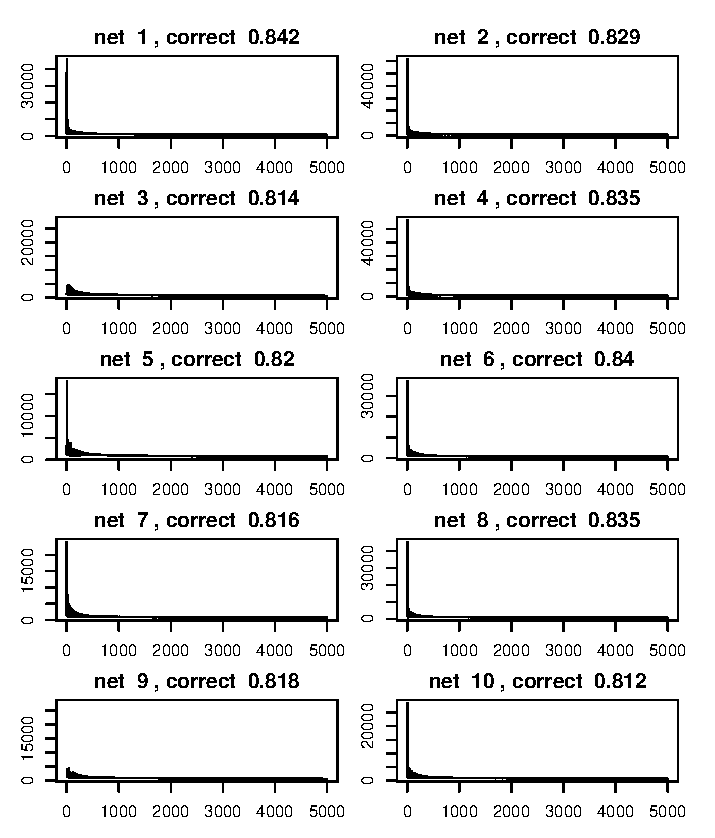
\includegraphics[width=5.5in]{04ANN/mammo3final1.eps}
\end{center}
\caption{ตัวอย่างโครงข่ายประสาทเทียมขนาด $30$ หน่วยย่อย ที่อัตราการเรียนรู้ $\rho_1 = 0.001$ และ $\rho_2 = 0.01$ และทำการฝึก $10$ ครั้ง.}
\label{fig: ann app final mamo}
\end{figure}
%

\subsubsection{ความเที่ยงตรง การเรียกกลับ และคะแนนเอฟ}

จากโมเดลที่ได้ ค่าความเที่ยงตรง ค่าการเรียกกลับ และค่าคะแนนเอฟ สามารถคำนวณได้ดังนี้
\begin{verbatim}
set2.y <- hardlimit(nnOutput(fnets[[1]], set2.Xn, nntype='biclass'))

true.pos <- sum( (set2.y == 1) & (set2.T == 1) )
true.neg <- sum( (set2.y == 0) & (set2.T == 0) )
false.pos <- sum( (set2.y == 1) & (set2.T == 0) )
false.neg <- sum( (set2.y == 0) & (set2.T == 1) )

r.precis <- true.pos/(true.pos + false.pos)
r.recall <- true.pos/(true.pos + false.neg)   
F.score <- 2*r.precis*r.recall/(r.precis + r.recall)
\end{verbatim}
โดย \texttt{accuracy}, \texttt{true.pos}, \texttt{true.neg}, \texttt{false.pos}, \texttt{false.neg}, \texttt{r.precis}, \texttt{r.recall}, และ \texttt{F.score} คือ ค่าความแม่นยำ, ค่าบวกจริง, ค่าลบจริง, ค่าบวกเท็จ, ค่าลบเท็จ, ค่าความเที่ยงตรง, ค่าการเรียกกลับ, และค่าคะแนนเอฟ ตามลำดับ.
ดูตาราง~\ref{tbl: ann app precision recall} ประกอบ.

\subsection{โค้ดสำหรับตัวอย่างการจำแนกกลุ่มแบบหลายกลุ่ม (ข้อมูลชุดรูปของลายมือเขียนตัวเลข)}
\label{sec: ann app multiclass code}


โค้ดสำหรับตัวอย่างข้อมูลชุดรูปของลายมือเขียนตัวเลขก็คล้ายๆกับตัวอย่างก่อนๆ.
สิ่งที่ต่างกันคือ (1) ตัวอย่างนี้เป็นงานการจำแนกกลุ่มแบบหลายกลุ่ม และ (2) มีการจัดการกับลักษณะเฉพาะของข้อมูล.

\subsubsection{โค้ดสำหรับการจำแนกกลุ่มแบบหลายกลุ่ม}

สำหรับงานการจำแนกกลุ่มแบบหลายกลุ่มจะใช้เอาต์พุตแบบ\textit{รหัสหนึ่งไปเค} (1-of-K Coding) 
และเพื่อความสะดวก ตัวอย่างนี้สร้างฟังชั่นเฉพาะ \texttt{encode.OK} และ \texttt{decode.OK} สำหรับการแปลงเอาต์พุตที่บอกค่ากลุ่มไปเป็น\textit{รหัสหนึ่งไปเค} และแปลงกลับ ตามลำดับ.
รายการ~\ref{lst: ANN makeIndicators} และ \ref{lst: ANN which.class} 
แสดงโค้ดของ \texttt{encode.OK} และ \texttt{decode.OK} ตามลำดับ.
ฟังชั่น \texttt{encode.OK} แปลงจากเอาต์พุต\textit{ค่าเดี่ยว} เช่น กลุ่ม `2' เป็น ค่า\textit{รหัสหนึ่งไปเค} ($K$ มิติ) เช่น $[01000]$.
ส่วนฟังชั่น \texttt{decode.OK} แปลงจากเอาต์พุตใน\textit{รหัสหนึ่งไปเค} เช่น $[01000]$ กลับเป็น\textit{ค่าเดี่ยว} เช่น `2'.

\begin{lstlisting}[language=R,caption={โค้ดฟังชั่น \texttt{encode.OK}},
label={lst: ANN makeIndicators}]
encode.OK <- function(T, classes=sort(unique(as.character(T)))){
  K <- length(classes)
  N <- length(T)

  T.K <- (matrix(T,K,N, byrow=TRUE) == 
          matrix(classes,K,N,byrow=FALSE))*1

  rownames(T.K) <- classes
  return(T.K)
}
\end{lstlisting}

\begin{lstlisting}[language=R,caption={โค้ดฟังชั่น \texttt{decode.OK}},
label={lst: ANN which.class}]
decode.OK <- function(Y.K, classes=rownames(Y.K)){
  if (is.null(classes)) {
    classes <- as.character(seq(1,nrow(Y.K)))
  }# end if

  Y.class <- classes[apply(Y.K, 2, which.max)]
  return(matrix(Y.class,nrow=1))
}
\end{lstlisting}

นอกจากนั้น โค้ดสำหรับโครงข่ายประสาทเทียมในรายการ
~\ref{lst: ann nntrain} ต้องปรับเปลี่ยนให้เหมาะกับงานการจำแนกกลุ่มแบบหลายกลุ่มด้วย (ดูตาราง~\ref{tbl: ANN output activation function} ประกอบ) โดยการปรับแก้\textit{ฟังชั่นกระตุ้นของชั้นเอาต์พุต}ให้เป็น\textit{ซอฟต์แมกซ์ฟังชั่น}.
นั่นคือ
การแก้ไข
บรรทัดที่ 36 ของ \texttt{nnTrain} ใน รายการ~\ref{lst: ann nntrain}
จาก \texttt{Y <- W2 \%*\% dotZ} เป็น
\begin{verbatim}
  A <- W2 %*% dotZ
  Y <- exp(A)/matrix(colSums(exp(A)), K, N, byrow=TRUE)  
\end{verbatim}

เช่นเดียวกับตัวอย่างการจำแนกกลุ่มแบบสองกลุ่ม การคำนวณค่าผิดพลาดอาจปรับแก้ให้เข้ากับงานจำแนกกลุ่มแบบหลายกลุ่ม (สมการ~\ref{eq: ann cost fn multiclass} ตามที่ถกในหัวข้อ~\ref{sec: ANN training}) ได้แก่ การแก้ไขบรรทัดที่ 53 ของ \texttt{nnTrain} ใน รายการ~\ref{lst: ann nntrain}
%จาก \texttt{errors[epoch+firstEpoch-1] <- sqrt(mean(DELTA2^2))} 
เป็น
\begin{verbatim}
errors[epoch+firstEpoch-1] <- -sum( T * log(Y) )   
\end{verbatim}

\subsubsection{โค้ดสำหรับการฝึกและทดสอบ}

การนำข้อมูลเข้าตัวแปรของอาร์โปรเจค และแปลงตัวแปรนี้ให้เป็นเมตริกซ์ สามารถทำได้ดังนี้
\begin{verbatim}
train.zip <- read.table('zip.train')
numzip <- apply(train.zip,c(1,2),as.numeric)
\end{verbatim}

สังเกตุ ตัวแปร \texttt{numzip} จะเป็นเมตริกซ์ขนาด $7291 \times  257$.
นั่นคือ ข้อมูลชุดนี้มี $7,291$ จุดข้อมูล และแต่ละจุดข้อมูลมี $257$ มิติ ($1$ มิติบอกว่าภาพเป็นภาพของเลขใด 
และ $256$ มิติสำหรับค่าของแต่ละพิกเซลของภาพ).
หากสำรวจดูค่าของตัวแปร \texttt{numzip} โดยคำสั่ง \texttt{summary(numzip)} จะเห็นว่าค่าของพิกเซล ถูกทำนอร์มอไลเซชั่นมาแล้ว (ค่าอยู่ในช่วง $[-1,1]$).
คอลัมน์แรกแทนเฉลย และ $256$ คอลัมน์ต่อมาเป็นค่าความเข้มของพิกเซลที่ถูกทำนอร์มอไลเซชั่นมาแล้ว.

ภาพของแต่ละจุดข้อมูลสามารถนำมาเรียงกลับเป็นภาพ เพื่อตรวจดูด้วยตาได้โดยใช้คำสั่ง \texttt{image}
เช่น 
\begin{verbatim}
image(seq(1,16), seq(1,16), t(apply(matrix(numzip[19,-1],16,16),1,rev)))
\end{verbatim} 
สำหรับดูรูปของจุดข้อมูลที่ 19.
สังเกตุว่า มีการตัดมิติที่ 1 ออก (\texttt{numzip[19,\textbf{-1}]}) 
เพราะมิติที่ 1 ของตัวแปรเป็นค่าเฉลยที่บอกกลุ่ม 
เช่นหากเรียก \texttt{numzip[19,1]} ก็ได้ค่าเฉลยออกมาว่าภาพในจุดข้อมูลที่ 19 นี้เป็นภาพของเลขใด.
ดังนั้น การแยกข้อมูลนี้ออกเป็นอินพุต \texttt{X} และเอาต์พุต \texttt{T} จึงทำดังนี้
\begin{verbatim}
X <- t(numzip[,-1])  # X is D x N
T <- t(numzip[,1])   # T is 1 x N
\end{verbatim}

ข้อมูลควรจัดสรรออกเป็นชุดฝึกและชุดวาลิเดชั่น ซึ่งสามารถทำได้ดังนี้
\begin{verbatim}
N <- ncol(X)
id.rand <- sample(N)

marker <- round(0.75*N)

train.X <- X[,id.rand[1:marker]]
train.T <- T[,id.rand[1:marker]]
train.T.K <- encode.OK(train.T)
  
validate.X <- X[,id.rand[-1:-marker]]
validate.T <- T[,id.rand[-1:-marker]]
validate.T.K <- encode.OK(validate.T)  
\end{verbatim}

ตัวอย่างนี้แยกราวๆ $75\%$ ของข้อมูลสำหรับการฝึก และที่เหลือสำหรับการทำวาลิเดชั่น.
ข้อมูลชุดนี้มีชุดข้อมูลสำหรับทดสอบแยกไว้ต่างหากอยู่แล้ว.
ซึ่งชุดข้อมูลสำหรับทดสอบ ก็สามารถโหลดมาได้ในลักษณะเดียวกัน
\begin{verbatim}
test.zip <- read.table('zip.test')
test.num <- apply(test.zip,c(1,2),as.numeric)

test.X <- t(test.zip[,-1])  # X is D x N
test.T <- t(test.zip[,1])   # T is 1 x N
\end{verbatim}

โครงข่ายประสาทเทียมสามารถถูกฝึกได้เช่นเดียวกับตัวอย่างที่ผ่านมา 
และ เพื่อความสะดวก ตัวอย่างนี้ใช้การเขียนเป็นลูป เพื่อทำการฝึกหลายๆครั้ง สำหรับการสุ่มค่าเริ่มต้นของค่าน้ำหนัก ดังนี้
\begin{verbatim}
records <- matrix(0, 1, 10)
nets <- vector('list', 10)

for(i in 1:10){

  nets[[i]] <- nnTrain(train.X,train.T.K, 
    nHiddens=40, rhoh=0.0002, rhoo=0.002, wmax=0.1, 
    nEpochs=500, net=NULL,
    earlystopping=TRUE, early.tol=1, 
    val.X=validate.X, val.T=validate.T.K)

  ## Test Network
  test.y <- nnOutput(nets[[i]],test.X, nntype='multiclass')
  Accuracy <- sum(
    decode.OK(test.y, c('0','1','2','3','4','5','6','7','8','9'))
    ==test.T)/N.test
  records[i] = Accuracy
}
\end{verbatim}

โค้ดข้างต้น แสดงตัวอย่างการฝึก $10$ ครั้ง 
เก็บโครงข่ายประสาทเทียมที่ฝึกแล้วทุกๆครั้ง (ซึ่งเก็บในตัวแปร \texttt{nets}).
\textit{โครงข่ายประสาทเทียมที่ฝึกได้ดีที่สุด}เลือกได้จากค่าความแม่นยำที่บันทึกไว้ในตัวแปร \texttt{records}.
แต่ก่อนจะเลือก \textit{ผู้เตรียมโครงข่ายประสาทเทียม}ควรตรวจสอบดูว่าผลการฝึกเป็นไปด้วยดีหรือไม่ 
เช่น ตรวจสอบดูว่า\textit{ค่าผิดพลาดระหว่างการฝึก}ลู่เข้าเรียบร้อยแล้ว ซึ่งอาจดูได้จากพล๊อตผลการฝึกทั้ง $10$ ครั้ง

โค้ดวาดพล๊อตผลการฝึกทั้ง $10$ ครั้ง ทำได้ดังนี้
\begin{verbatim}
p=par(mfrow=c(2,5))
for(i in 1:10){
  N = max(which(nets[[i]]$errors > 0))
  plot(1:N, nets[[i]]$errors[1:N], xlab='epoch', ylab='cost',
   type='l', main= paste('Train ', i, 
    ';\nTest\'s correct ', round(records[i],2)))
}
par(p)
\end{verbatim}

รูป~\ref{fig: ann zip m 40 high rhos} และ \ref{fig: ann zip m 40 good rhos} แสดงตัวอย่างการตรวจสอบการฝึก.
%
หากการฝึกมีปัญหา ก็ควรปรับปรุงแก้ไขให้เรียบร้อยก่อน เช่น หากค่าอัตราการเรียนรู้มากเกินไป ก็ปรับลดลงมา
หรือหากผลการฝึกดูเหมือนต้องการรอบฝึกเพิ่ม ก็ควรปรับแก้ไขเพิ่มรอบฝึกขึ้นตามความเหมาะสมกับสถานะการณ์.

เมื่อผลการฝึกดูเรียบร้อยดี ผู้เตรียมโครงข่ายประสาทเทียมก็จะสามารถเลือกโครงข่ายประสาทเทียมจากครั้งที่ได้ผลดีที่สุด 
เช่น เมื่อการฝึกครั้งที่ 2 ให้ผลดีที่สุด ตัวอย่างนี้ก็เลือกโครงข่ายที่เก็บในตัวแปร \texttt{nets[[2]]} มาใช้งาน. 
ตัวอย่างโค้ดข้างล่างเก็บโครงข่ายประสาทเทียมนี้ไว้ใช้งานต่อไปในไฟล์ \texttt{chosenNet.RData} ดังนี้
\begin{verbatim}
net <- nets[[2]]
save(net, file='chosenNet.RData')
\end{verbatim}

เมื่อต้องการนำโครงข่ายประสาทเทียมมาใช้งาน ก็เพียงแต่เรียก
\begin{verbatim}
load('chosenNet.RData')
\end{verbatim}

จากนั้นก็สามารถนำตัวแปรที่บันทึกไว้ (ตัวแปร \texttt{net}) ไปใช้งานได้เลย 
เช่น สามารถเรียกใช้ \texttt{nnOutput(net,} {\small \textit{อินพุตที่สงสัย}}\texttt{, nntype='multiclass')} เพื่อทำนายกลุ่มจากค่า{\small \textit{อินพุตที่สงสัย}}.
หัวข้อ~\ref{sec: ann app freedraw} แสดงตัวอย่างแอพพลิเคชั่นง่ายๆที่ใช้โครงข่ายประสาทเทียมที่บันทึกเก็บไว้นี้.

\subsubsection{โค้ดสำหรับทดลองโปรแกรมใช้งานโครงข่ายประสาทเทียม}
\label{sec: ann app freedraw}

โค้ดในรายการ~\ref{lst: ann freeDraw} เมื่อรัน โดยการเรียก \texttt{source('freeDraw.r')} โปรแกรมจะเปิด\textit{หน้าต่างรับอินพุต}ขึ้นมา (รูป~\ref{fig: ANN freedraw pad}).
ที่หน้าต่างรับอินพุต ผู้ใช้สามารถเขียนตัวเลขที่ต้องการลงไปได้โดยใช้\textit{เมาส์}.
การเขียนตัวเลข เริ่มโดยการ\textit{คลิกขวา}ครั้งแรก เพื่อบอกการเริ่มเขียน 
แล้วจึงลากเมาส์เพื่อเขียนเลข (ไม่จำเป็นกดปุ่มใดๆ)
และเมื่อต้องการหยุดเขียนให้คลิกเมาส์อีกครั้ง. 
ผู้ใช้สามารถเริ่มเขียนและหยุดเขียนได้ตลอด โดยคลิกขวาเพื่อสลับระหว่างการเขียนและหยุดเขียน.
จนเมื่อเขียนเสร็จและต้องการให้โปรแกรมอ่านว่าเป็นเลขใด ให้กดคีย์บนคีย์บอร์ด (คีย์ใดก็ได้ เช่น `q', `w', `e', ...).
รูป~\ref{fig: ANN freedraw pad} แสดงตัวอย่างหน้าต่างรับอินพุตที่วาดเลข 4 ลงไปแล้ว.
เมื่อกดคีย์ โปรแกรมจะอ่านออกมาว่าเป็นภาพที่วาดเป็นภาพของเลขใด.
ตัวอย่างผลแสดงดังรูป~\ref{fig: ANN freedraw results}.

%
\begin{figure}
\begin{center}
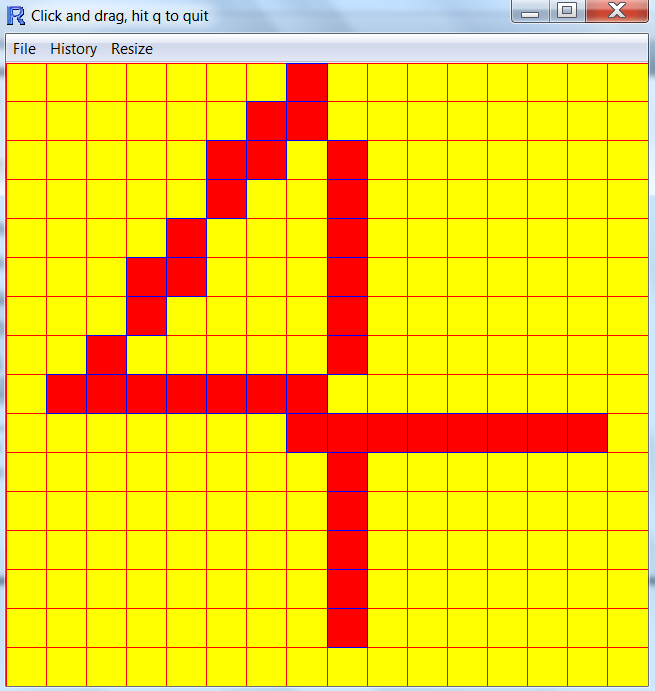
\includegraphics[height=3in]{04ANNAppImg/freeDrawPad.png}
\end{center}
\caption{ตัวอย่างหน้าต่างรับอินพุตที่ผู้ใช้วาดเลข 4 ลงไป.}
\label{fig: ANN freedraw pad}
\end{figure}
%

%
\begin{figure}
\begin{center}
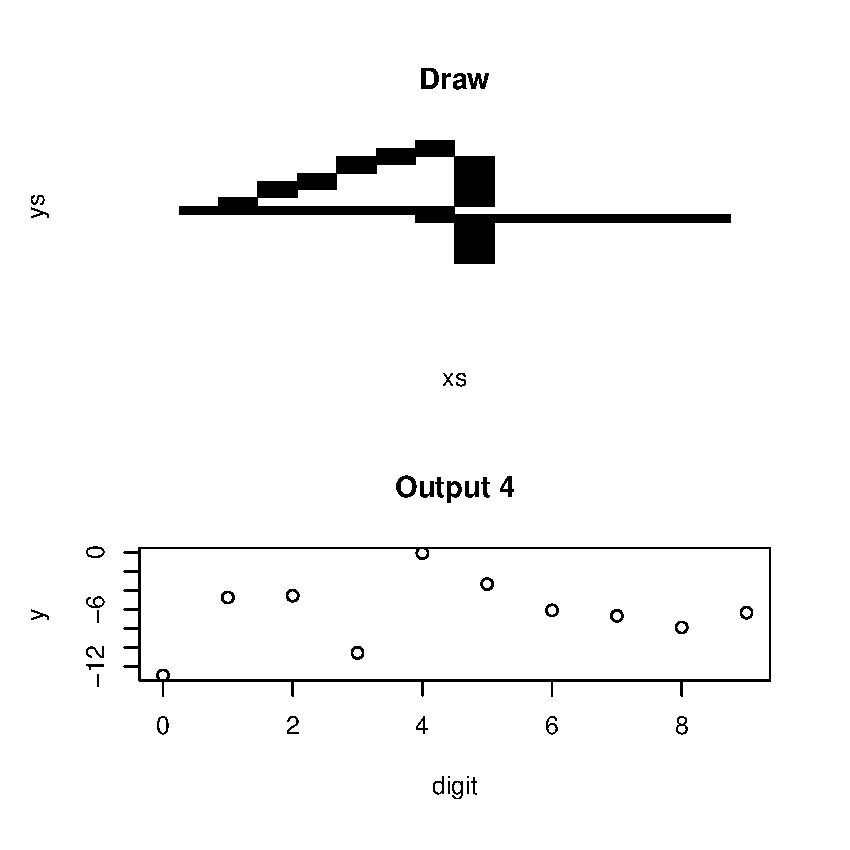
\includegraphics[height=3in]{04ANNAppImg/freeDrawResult.eps}
\end{center}
\caption{ตัวอย่างผลจากโปรแกรม \texttt{freeDraw}. 
ภาพบนแสดงภาพที่ผู้ใช้วาด.
ภาพล่างแสดงค่าซอฟต์แมกซ์ของทั้งสิบกลุ่ม และโครงข่ายประสาทเทียมจะเลือกทายเป็นกลุ่มที่มีค่าซอฟต์แมกซ์นี้สูงที่สุด ซึ่งในภาพนี้คือกลุ่มของตัวเลข `4'.}
\label{fig: ANN freedraw results}
\end{figure}
%

โค้ดโปรแกรม \texttt{freeDraw} (รายการ~\ref{lst: ann freeDraw}) เรียกใช้ \texttt{library(grid)} สำหรับทำกราฟฟิกส์ และการโหลดโครงข่ายประสาทเทียมที่ฝึกไว้แล้วทำในบรรทัดที่ 10.
โปรแกรม \texttt{freeDraw} เรียกใช้ ฟังชั่นต่างๆที่ได้อภิปรายไปแล้ว เช่น \texttt{nnOutput}, \texttt{sigmoid}, \texttt{decode.OK}.
ตัวโปรแกรมจะเริ่มด้วยการเปิด\textit{หน้าต่างรับอินพุต} (บรรทัด 90-104)
แล้วลงทะเบียนฟังชั่นสำหรับจัดการอีเวนต์ (บรรทัด 203-206) โดยลงทะเบียนฟังชั่นต่างๆที่สำหรับจัดการอีเวนต์ ได้แก่ 
\begin{itemize}
\item ฟังชั่น \texttt{dragmousedown} สำหรับการคลิกเมาส์ ซึ่งจะสลับระหว่างการเริ่มวาดและการหยุดวาด. 
หากเริ่มวาด ฟังชั่น \texttt{dragmousedown} จะวาดตำแหน่งของเมาส์บนหน้าต่างรับอินพุต และลงทะเบียนฟังชั่น \texttt{dragmousemove} สำหรับอีเวนต์ที่มีการเลื่อนเมาส์ (บรรทัด 171).
แต่หากหยุดวาด ก็จะถอนการละเบียนรับอีเวนต์การเลื่อนเมาส์ออก (บรรทัด 177).
ฟังชั่น \texttt{dragmousedown} ใช้ตัวแปร \texttt{write.on} เก็บสถานะของหน้าต่างว่าอยู่ในสถานะ``วาด'' หรือ ``หยุดวาด''
\\
ตัวแปรที่ใช้เก็บค่าของภาพที่วาด (ค่าของพิกเซลขนาด $16 \times 16$) คือ ต้วแปร \texttt{zs} ประกาศในบรรทัด 55 ด้วยค่าเริ่มต้นเป็น $0$ สำหรับทุกพิกเซล.
สังเกตุการกำหนดค่าสำหรับตัวแปรที่เป็นตัวแปรส่วนกลาง (global variable) ที่ใช้ตัวปฏิบัติการ \texttt{<<-} แทน \texttt{<-} หรือ \texttt{=}.
%ที่จะเก็บค่าของพิกเซล (เป็น $0$ หรือ $1$) ตามตำแหน่งของเมาส์ที่วาด.
ค่าใน \texttt{zs} จะถูกเซต ด้วยฟังชั่น \texttt{setZ}.
บรรทัด 111-112 ของฟังชั่น \texttt{setZ} ทำการแปลงจากตำแหน่งของเมาส์ มาเป็นตำแหน่งของพิกเซล ก่อนที่จะเซตค่าของ \texttt{zs} ที่ตรงกับตำแหน่งพิกเซลนั้น (บรรทัด 114).
ฟังชั่น \texttt{setZ} จะถูกเรียก เมื่อฟังชั่น \texttt{dragmousedown} เริ่มวาด (บรรทัด 173) หรือ \texttt{drawmousemove} ทำงาน (บรรทัด 186).
ฟังชั่น \texttt{drawZ} จะวาดภาพในหน้าต่างรับอินพุตใหม่ให้ตอบสนองการเปลี่ยนแปลง.
\item ฟังชั่น \texttt{keydown} สำหรับจัดการ\textit{การกดคีย์} ซึ่งจะเรียกฟังชั่น \texttt{draw.off} (บรรทัด 61-78) มาทำงาน. 
ฟังชั่น \texttt{draw.off} จะนำ\textit{ภาพที่ผู้ใช้วาด}%
มาจัดเรียง และแปลงค่าให้อยู่ในรูปแบบอินพุตของโครงข่ายประสาทเทียม (บรรทัด 67)
ก่อนจะเรียกใช้โครงข่ายประสาทเทียมเพื่อจำแนกว่า\textit{ภาพที่วาด}เป็นภาพของเลขใด (บรรทัด 70) 
และแสดงผลออกมา (บรรทัด 72-74).
\end{itemize}

สำหรับรายละเอียดการโปรแกรมอาร์โปรเจคแบบอีเวนต์ดริฟเฟน (event-driven) ผู้อ่านสามารถศึกษาเพิ่มเติมได้จาก \texttt{help(getGraphicsEvent)} และการจัดการกราฟฟิกส์ในโปรแกรม \texttt{freeDraw} ก็สามารถศึกษาเพิ่มเติมได้จาก \texttt{help(grid.polygon)} และ \texttt{help(grid.rect)}.

\lstinputlisting[language=R, caption={โค้ดโปรแกรม \texttt{freeDraw} (ให้ตั้งชื่อไฟล์เป็น \texttt{freeDraw.r})}, 
label={lst: ann freeDraw}]{04ANNAppImg/freeDrawCode.r}

โปรแกรม \texttt{freeDraw} นี้เป็นโปรแกรมสั้นๆ เพื่อแสดงให้เห็นการนำโมเดลที่ฝึกแล้วไปใช้งาน.
หลังจากได้โมเดลแล้ว ผู้พัฒนาโปรแกรมไม่จำเป็นต้องทำการฝึกอีก ดังตัวอย่างในโปรแกรม \texttt{freeDraw} นี้.
แต่หากผู้พัฒนาโปรแกรมต้องการให้แอพพลิเคชั่นสามารถปรับปรุงตัวเองได้ตลอด 
เช่น หากผู้ใช้เขียนออกไปแล้ว โปรแกรมอ่านเป็นตัวเลขผิด 
ผู้ใช้อาจจะกดลบแล้ววาดใหม่ หรือผู้ใช้อาจจะเลือกพิมพ์เข้าไปแทน ซึ่งพฤติกรรมเหล่านี้สามารถตรวจจับได้และ ก็สามารถเพิ่มการเรียนรู้เข้าไป เพื่อทำให้โปรแกรมทำงานได้ดีขึ้นได้
หรือแม้แต่การเรียงกลุ่มที่มีค่าซอฟต์แมกซ์สูงสุด และให้ผู้ใช้เลือกกลุ่มที่ถูกต้อง ก็จะสามารถได้รับเฉลยจากผู้ใช้ตลอดการใช้งาน โดยที่ไม่รบกวนผู้ใช้มากเกินไป.
%
%ตัวอย่างต่างๆในบทนี้คงช่วยให้ผู้อ่าน มองเห็นภาพ การทำเทคนิคการเรียนรู้ของเครื่องไปใช้งาน ได้บ้าง, ไม่ว่าจะเป็น งานพัฒนาแอพพลิเคชั่น หรือ งานศึกษาวิจัย.

\section{แบบฝึกหัด}
\label{section: ANN exercises}
\paragraph{1.} 
จงเลือกชุดข้อมูลมาสำหรับการหาค่าถดถอย $1$ ชุด สำหรับการแบ่งกลุ่ม $1$ ชุด,
เปรียบเทียบผลการใช้โครงข่ายประสาทเทียม ในแง่มุมของการใช้\textit{จำนวนหน่วยซ่อน}ต่างๆ \textit{ค่าอัตราการเรียนรู้}ต่างๆ และ\textit{จำนวนรอบฝึก}ต่างๆ.
อภิปรายความสัมพันธ์ของ\textit{จำนวนหน่วยซ่อน}, \textit{ค่าอัตราการเรียนรู้}ของชั้นซ่อนและชั้นเอาต์พุต และ\textit{จำนวนรอบฝึก}ในเรื่องผลการทำงาน.

\paragraph{2.} 
จงเลือกชุดข้อมูลมาสำหรับการหาค่าถดถอย $2$ ชุด สำหรับการแบ่งกลุ่ม $2$ ชุด,
เปรียบเทียบ\textit{การสุ่มค่าเริ่มต้น}ให้กับโครงข่ายประสาทเทียมแบบต่างๆ เช่นสุ่มจากกระจายรูปเดี่ยว (uniform distribution) ที่ช่วงค่าต่างๆ (ค่า \texttt{wmax} ในรายการ~\ref{lst: ann nnOutput}) 
หรือสุ่มจากการกระจายปกติ (normal distribution) ที่ใช้ค่าเบี่ยงเบนมาตราฐานต่างๆ.
อภิปรายผลที่ได้.

\paragraph{3.} 
จงเลือกชุดข้อมูลมาสำหรับการหาค่าถดถอย $2$ ชุด สำหรับการแบ่งกลุ่ม $2$ ชุด,
เปรียบเทียบการใช้โครงข่ายประสาทเทียมที่มีการทำนอร์มอไลเซชั่นกับข้อมูล กับการใช้โครงข่ายประสาทเทียมที่ไม่มีการทำนอร์มอไลเซชั่น.
อภิปรายผลที่ได้.

\paragraph{4.}
จากแบบฝึกหัดข้อ 4 บท~\ref{chapter: ANN} จงดัดแปลงโค้ดของ \texttt{nnTrain} (รายการ~\ref{lst: ann nntrain}) เพื่อให้รองรับการทำเรกูลาไรเซชั่น.
คำใบ้ \texttt{dE2} และ \texttt{dE1} ใน บรรทัด 46 และ 47 (รายการ~\ref{lst: ann nntrain}) คือ $\frac{\partial E_n}{\partial w_{ji}^{(2)}}$ และ $\frac{\partial E_n}{\partial w_{ji}^{(1)}}$, ดูสมการ~\ref{eq: ann regularized derivative 2} และ \ref{eq: ann regularized derivative 1} ประกอบ.

\paragraph{5.}
จากตัวอย่างในหัวข้อ~\ref{sec: simple example} จงทดลองทำใหม่ด้วย\textit{โครงข่ายประสาทเทียม}%
กับการฝึกที่ใช้เรกูลาไรเซชั่น ให้ทดลองค่า $\lambda_1$ และ $\lambda_2$ หลายๆค่า เช่น $0, 0.000001, 0.001, 1, 10$ เป็นต้น.
จงอภิปรายผลโดยเฉพาะความสัมพันธ์ของค่า $\lambda_1$ และ $\lambda_2$ กับผลการทำนายที่ได้.

\paragraph{6.} 
จงเลือกชุดข้อมูลมา $3$ ชุดสำหรับการหาค่าถดถอย 
และใช้โครงข่ายประสาทเทียมในการทำโมเดลและการประเมินผล.
จงเปรียบเทียบและอภิปรายผลระหว่างการใช้\textit{การหยุดก่อนกำหนด} (Early Stopping), \textit{การทำเรกูลาไรเซชั่น} (Regularization) และการที่ไม่ใช้ทั้งสองอย่าง.
%จงอภิปรายผลการใช้ การหยุดก่อนกำหนด (Early Stopping), การทำเรกูลาไรเซชั่น (Regularization) และ ไม่ใช้ทั้งสองอย่าง กับการใช้ โครงข่ายประสาทเทียม สำหรับ การหาค่าถดถอย.

\paragraph{7.} 
จงเลือกชุดข้อมูลมา $3$ ชุดสำหรับการจำแนกกลุ่ม
และใช้โครงข่ายประสาทเทียมในการทำโมเดลและการประเมินผล.
จงเปรียบเทียบและอภิปรายผลการใช้การหยุดก่อนกำหนด, การทำเรกูลาไรเซชั่น และการที่ไม่ใช้ทั้งสองอย่าง.

\paragraph{8.} 
%จากตัวอย่างข้อมูลชุดภาพเอ็กซเรย์เต้านมของมวลเนื้อ 
จงเลือกชุดข้อมูล $3$ ชุดที่แต่ละชุดมีเขตข้อมูลบางเขตขาดหาย
และจงเปรียบเทียบ อภิปรายผล จากวิธีจัดการกับเขตข้อมูลบางเขตขาดหาย วิธีต่างๆ ได้แก่ 
วิธีการตัดระเบียนที่มีเขตข้อมูลขาดหาย 
วิธีการแทนค่าที่ขาดหายด้วยทุกค่าที่เป็นไปได้
วิธีการแทนค่าที่ขาดหายไปด้วยค่าเฉลี่ยหรือค่าที่พบบ่อยที่สุด.

\paragraph{9.}
จงศึกษาผลของการที่มีข้อมูลขาดหาย โดยเลือกชุดข้อมูลที่ไม่มีเขตข้อมูลขาดหาย (no missing data) มา $1$ ชุด แล้วทดลองสร้างชุดข้อมูลใหม่ $5$ ชุด  โดยที่แต่ละชุดสร้างจากข้อมูลต้นฉบับ แต่สุ่มละค่าบางค่าของข้อมูลออกไป $0.1\%$, $1\%$, $10\%$, $20\%$, และ $40\%$.
ให้ใช้โครงข่างประสาทเทียมทำโมเดลกับข้อมูลทั้ง $6$ ชุดนี้ (รวมต้นฉบับด้วย) ประเมินผล และเปรียบเทียบ.
ให้เลือกวิธีใช้วิธีจัดการกับข้อมูลขาดหาย พร้อมอธิบายเหตุผล.
จงอภิปรายความสัมพันธ์ระหว่างปริมาณข้อมูลขาดหายและผลการทำนาย.
(ดูตัวอย่างจาก \cite{JuholaLaurikkala2013a})

\paragraph{10.}
จงออกแบบการทดลอง เพื่อเปรียบเทียบผลของการใช้\textit{วาลิเดชั่น} (แบ่งสองกลุ่มทำทีเดียว) 
กับผลของการใช้\textit{ครอสวาลิเดชั่น} (แบ่งเป็นหลายพับและทำเท่าจำนวนพับครั้ง) โดยเฉพาะปัจจัยที่ขนาดข้อมูลต่างๆ.
คำแนะนำ ให้ใช้ข้อมูลอย่างน้อย $3$ ชุด และเลือกให้ข้อมูลมีความยากง่ายต่างกัน.
และจากข้อมูล $3$ ชุดหลัก ให้สร้างชุดข้อมูลใหม่ที่ขนาดเล็กลง จากการสุ่มจากชุดข้อมูลเดิม เพื่อใช้ในการศึกษาผลที่ปริมาณข้อมูลต่างกัน.

\paragraph{11.}
จากวิธีคำนวณค่าเกรเดียนต์เชิงเลข
\begin{eqnarray}
\nabla_{\theta} J(\theta) = 
\begin{bmatrix}
  \frac{\partial J}{\partial \theta_1} \\
  \frac{\partial J}{\partial \theta_2} \\  
  \vdots \\
  \frac{\partial J}{\partial \theta_M} \\   
\end{bmatrix},
\mbox{ และ }
  \frac{\partial J}{\partial \theta_i} \approx
  \frac{J(\begin{bmatrix}
  \vdots \\
  \theta_{i-1} \\
  \theta_i + \epsilon \\
  \theta_{i+1} \\
  \vdots \\  
  \end{bmatrix})
   - J(\begin{bmatrix}
  \vdots \\
  \theta_{i-1} \\
  \theta_i - \epsilon \\
  \theta_{i+1} \\
  \vdots \\  
  \end{bmatrix})}{2 \epsilon}
\label{eq: ann app numerical grad}  
\end{eqnarray}
เมื่อ $J(\theta)$ คือค่าฟังชั่นจุดประสงค์.
สำหรับปัญหา $3$ แบบ ได้แก่ การหาค่าถดถอย การจำแนกกลุ่มแบบสองกลุ่ม และการจำแนกกลุ่มแบบหลายกลุ่ม, 
จงทดสอบ\textit{ค่าเกรเดียนต์ที่คำนวณจากวิธีแพร่กระจาย}เปรียบเทียบกับ\textit{ค่าเกรเดียนต์ที่คำนวณจากวิธีการเชิงเลข} (ดูโค้ดในรายการ~\ref{lst: ann app numericalGrad})
โดยให้ใช้ค่า $\epsilon$ เป็น $1$, $0.01$ และ $0.0001$ ตามลำดับ.
จงสรุปและอภิปรายผล.

\underline{คำใบ้} ดูตัวอย่างโค้ดวิธีตรวจสอบจากรายการ~\ref{lst: ann app checkNumericalGrad02.r}.
หากทุกอย่างถูกต้อง ค่าเกรเดียนต์ที่คำนวณจากการวิเคราะห์ \texttt{fn.grad} ควรจะใกล้เคียงมากๆกับค่าเกรเดียนต์ ที่ประมาณจากการคำนวณเชิงเลข \texttt{num.vals}.

\lstinputlisting[language=R, caption={ฟังชั่น \texttt{numericalGrad}. โค้ดตัวอย่างการคำนวณค่าเกรเดียนต์จากฟังชั่นจุดประสงค์ด้วยวิธีเชิงเลข
การคำนวณด้วยวิธีเชิงเลขทำเพื่อใช้ตรวจสอบความถูกต้องของโค้ดการแพร่กระจายย้อนกลับ}, 
label={lst: ann app numericalGrad}]{src/cfNumGrad/numericalGradCode.r}

\begin{lstlisting}[language=R,caption={ตัวอย่างการเปรียบเทียบค่าเกรเดียนต์กับค่าประมาณเกรเดียนต์ด้วยวิธีเชิงเลข},
label={lst: ann app checkNumericalGrad02.r}]
quadratic.fn <- function(x){
  val = x[1]^2 + 3*x[1]*x[2]  
  grad = matrix(0, 2, 1)
  grad[1] = 2*x[1] + 3*x[2]
  grad[2] = 3*x[1]
return(list(cost=val, grad=grad))
}##end quadratic.fn

  x = matrix(c(4, 10), 2, 1)
  quad.vals <- quadratic.fn(x)

  fn.cost <- quad.vals$cost
  fn.grad <- quad.vals$grad

  num.vals <- numericalGrad(function(a){quadratic.fn(a)$cost}, x, epsilon=0.01)
\end{lstlisting}

\paragraph{12.}
จงเลือกชุดข้อมูล $1$ ชุด
แล้วเลือก เตรียม ฝึก และทดสอบโครงข่ายประสาทเทียมให้ได้ผลการทำงานที่ดี
และแสดงผลการทำนายของโครงข่ายประสาทเทียมเปรียบเทียบกับค่าเอาต์พุตของหน่วยซ่อนต่างๆ
สรุปผล และอภิปรายความสัมพันธ์ของค่าเอาต์พุตของหน่วยซ่อนต่างๆกับการทำงานของโครงข่ายประสาทเทียม.
